\documentclass[11pt,a4paper,oldfontcommands,openany]{memoir}
\usepackage{graphicx}
\usepackage[]{color}
\usepackage{courier}
\usepackage[usenames,dvipsnames]{xcolor}
\usepackage[breakable, theorems, skins]{tcolorbox}
\usepackage[]{media9}
\usepackage{lipsum}
\usepackage{pdfpages}
\tcbset{enhanced}
%% maxwidth is the original width if it is less than linewidth
%% otherwise use linewidth (to make sure the graphics do not exceed the margin)
\makeatletter
\def\maxwidth{ %
  \ifdim\Gin@nat@width>\linewidth
    \linewidth
  \else
    \Gin@nat@width
  \fi
}
\makeatother

\DeclareRobustCommand{\mybox}[2][gray!15]{%
\begin{tcolorbox}[   %% Adjust the following parameters at will.
        breakable,
        left=0pt,
        right=0pt,
        top=0pt,
        bottom=0pt,
        colback=#1,
        colframe=#1,
        width=\dimexpr\textwidth\relax, 
        enlarge left by=0mm,
        boxsep=5pt,
        arc=0pt,outer arc=0pt,
        ]
        #2
\end{tcolorbox}
}


\definecolor{fgcolor}{rgb}{0.345, 0.345, 0.345}
\newcommand{\hlnum}[1]{\textcolor[rgb]{0.686,0.059,0.569}{#1}}%
\newcommand{\hlstr}[1]{\textcolor[rgb]{0.192,0.494,0.8}{#1}}%
\newcommand{\hlcom}[1]{\textcolor[rgb]{0.678,0.584,0.686}{\textit{#1}}}%
\newcommand{\hlopt}[1]{\textcolor[rgb]{0,0,0}{#1}}%
\newcommand{\hlstd}[1]{\textcolor[rgb]{0.345,0.345,0.345}{#1}}%
\newcommand{\hlkwa}[1]{\textcolor[rgb]{0.161,0.373,0.58}{\textbf{#1}}}%
\newcommand{\hlkwb}[1]{\textcolor[rgb]{0.69,0.353,0.396}{#1}}%
\newcommand{\hlkwc}[1]{\textcolor[rgb]{0.333,0.667,0.333}{#1}}%
\newcommand{\hlkwd}[1]{\textcolor[rgb]{0.737,0.353,0.396}{\textbf{#1}}}%

\usepackage{framed}
\makeatletter
\newenvironment{kframe}{%
 \def\at@end@of@kframe{}%
 \ifinner\ifhmode%
  \def\at@end@of@kframe{\end{minipage}}%
  \begin{minipage}{\columnwidth}%
 \fi\fi%
 \def\FrameCommand##1{\hskip\@totalleftmargin \hskip-\fboxsep
 \colorbox{shadecolor}{##1}\hskip-\fboxsep
     % There is no \\@totalrightmargin, so:
     \hskip-\linewidth \hskip-\@totalleftmargin \hskip\columnwidth}%
 \MakeFramed {\advance\hsize-\width
   \@totalleftmargin\z@ \linewidth\hsize
   \@setminipage}}%
 {\par\unskip\endMakeFramed%
 \at@end@of@kframe}
\makeatother

\definecolor{shadecolor}{rgb}{.97, .97, .97}
\definecolor{messagecolor}{rgb}{0, 0, 0}
\definecolor{warningcolor}{rgb}{1, 0, 1}
\definecolor{errorcolor}{rgb}{1, 0, 0}
\newenvironment{knitrout}{}{} % an empty environment to be redefined in TeX

\usepackage{alltt}
\setlength{\parindent}{0pt} % Remove indent at new paragraphs
\setcounter{secnumdepth}{4}  % Remove section numbering at certain depth # If zero, then no numbering of sections
\setcounter{tocdepth}{4} % Determines number of subsections that will have tabs
\usepackage{tabu}
\usepackage{url}

\usepackage[round]{natbib}   % omit 'round' option if you prefer square brackets
\bibliographystyle{plainnat}

\usepackage{fixltx2e}
%\usepackage{graphicx}	% For external pictures
\usepackage{float}
\usepackage{subfig}	% Add subfigures within figures
\usepackage{verbatim}
\usepackage[colorlinks=true,linkcolor=blue,citecolor=blue,urlcolor=blue]{hyperref}
\usepackage{amssymb,amsbsy,amsmath}
\usepackage{epsfig}
\usepackage[left=3cm,top=3cm,bottom=3.5cm,right=3cm]{geometry} % For easy document margins
%\usepackage{fancyhdr} % For customization of header/footer
\usepackage{adjustbox}
\usepackage{framed}
\usepackage{enumitem}
\usepackage{caption}
\numberwithin{equation}{section} % Equation numbers relative to sections

%%%%% NEW ADDED FROM THESIS.TEX %%%%% 
\usepackage[utf8]{inputenc}
\usepackage[T1]{fontenc}
\usepackage{microtype}
%\usepackage[dvips]{graphicx}
%\usepackage{times} %clash
%%%%%%%%%%%%%%%%%%%%%%%%%%%%%%%%%%%%%%%% 
\newcommand{\code}[1]{{\texttt{#1}}}
\newcommand{\pkg}[1]{{\texttt{#1}}}
\newcommand{\class}[1]{{\textit{#1}}}
\newcommand{\R}{{\normalfont\textsf{R }}{}}
\IfFileExists{upquote.sty}{\usepackage{upquote}}{}


\begin{document}

\sloppy

%%%%%%%%%%%%%%%%%%%%% TITLE PAGE %%%%%%%%%%%%%%%%%%%%%

{
\centering
~\vspace{\fill}

\vspace{2.5cm}



\vspace{1cm}

{\LARGE\textbf{Visualization methods for genealogical and RNA-sequencing datasets}}

\vspace{1cm}

{\LARGE Lindsay Rutter}

\vspace{4cm}

{\LARGE Program of Study Committee:}

\vspace{1cm}

{\LARGE Dianne Cook (Major Professor)}

\vspace{.25cm}

{\LARGE Amy Toth (Major Professor)}

\vspace{.25cm}

{\LARGE Heike Hofmann}

\vspace{.25cm}

{\LARGE Daniel Nettleton}

\vspace{.25cm}

{\LARGE James Reecy}

\vspace{2.5cm}

{\centerline{\large May 1, 2018}}
}

\clearpage
%\cleardoublepage

%%% CHAPTER'S STYLE
\chapterstyle{bianchi}
\setsecheadstyle{\Large\bfseries\sffamily\raggedright}
\setsubsecheadstyle{\large\bfseries\sffamily\raggedright}
\setsubsubsecheadstyle{\bfseries\sffamily\raggedright}
%%%%%%%%%%%%%%%%%%%%%%%%%%%%%%%%%%%%

\tableofcontents

\setlength{\parskip}{10pt} % Inter-paragraph spacing

%%% ADDED FROM THESIS.TEX %%%%%%%%%
\OnehalfSpacing

\chapter{Introduction}
%%%%%%%%%%%%%%%%%%%%%%%%%%%%%%%%%%%%%%%%%%%%%%%%%%%%%%%%%%%%%%%%%%%
%%%%%%%%%%%%%%%%%%%%%%%%%%%%%%%%%%%%%%%%%%%%%%%%%%%%%%%%%%%%%%%%%%%
\section{Background to data visualization}

The problem with only applying traditional modeling approaches to data is that these models are replete with assumptions that they alone cannot call into question. Fortunately, visualization enables analysts to see things they may not have expected with traditional modeling. By plotting the data, analysts can determine whether or not the applied models are sensible; they can work between visualizations and modeling, enhancing the models based on feedback from the visuals. In sum, graphics are essential for analysts to check the quality of the data, assess the model diagnostics, and compare results from different methods.

%%%%%%%%%%%%%%%%%%%%%%%%%%%%%%%%%%%%%%%%%%%%%%%%%%%%%%%%%%%%%%%%%%%
%%%%%%%%%%%%%%%%%%%%%%%%%%%%%%%%%%%%%%%%%%%%%%%%%%%%%%%%%%%%%%%%%%%
\section{Problems to be addressed}

Genealogical data has a standardized type of display known as a pedigree chart, which we introduce in Section \ref{sec:litReview} (\citealt{ped}). While this visual plot is useful for certain genealogical datasets, it is not useful for many genealogical datasets, particularly agricultural ones that are used for breeding purposes. We address this problem by introducing a new type of plot to display the paths between the ancestors and descendants constrained by generation for an individual of interest, which could otherwise not be accomplished with a pedigree chart. This new plot (and other plots) are introduced in Chapter \ref{sec:chapter1}.

There are popular plotting tools for analyzing RNA-sequencing data, but there are less popular tools that could be more helpful for RNA-sequencing analysis. We strive to work on the following three uncommon plotting types that could be useful for better understanding RNA-sequencing data, and we show our accomplishments toward these goals in Chapters \ref{sec:chapter2}, \ref{sec:chapter3}, and \ref{sec:chapter4}:

\clearpage

\begin{enumerate}
\item \textbf{Parallel coordinate plots}:

In gene expression data analysis, we are striving to find relative patterns. Side-by-side boxplots are often used for this purpose, but they can hide potential problems that could still be lurking in the data after normalization. This is because most RNA-sequencing normalization methods are conducted at the sample-level, and side-by-side boxplots do not show connections between the samples. Consequently, boxplots may deceive analysts to believe that the normalization succeeded in cases where alternative plots (such as parallel coordinate plots) would have otherwise indicated that the normalization was in fact unsuccessful due to the presence of inconsistencies (crossings) between replicates. For this reason, parallel coordinate plots (\citealt{origPCP}, \citealt{origPCP2}) are an essential visual tool when checking the initial normalization process of RNA-sequencing analysis. If the normalization is adequate, then the connections between replications should be flat, and we should only see crossings between treatment groups.

The tools currently available for constructing parallel coordinate plots to assess RNA-sequencing data are severely limited: Namely, the large number of genes present can cause constraints in space and time. With one line being drawn for each gene, our resulting plots will have too many lines being drawn to even view patterns of interest in the first place. Moreover, the construction of these plots can be consuming in computation and time, often requiring analysts to wait for minutes before they can view the output. Even though popular tools to visualize parallel coordinate plots (such as the \code{ggparcoord} function in the \code{GGally} package) can be very useful for many datasets, they are not always helpful for large RNA-sequencing datasets (\citealt{ggally}).

As a result, we developed new approaches that both quickly and meaningfully displays the key pieces of information for RNA-sequencing data with parallel coordinate plots. First, we applied parallel coordinate plots after hierarchical analysis to reduce overlapping issues. We introduce the use of these tools in Chapter~\ref{sec:chapter2} as a case study applied to real RNA-sequencing data. We also apply them again in Chapter~\ref{sec:chapter4} as part of our study of virus and diet quality effects on honey bee gene expression. Second, we created interactive capabilities for parallel coordinate plots, wherein users can select lines more efficiently and keep and/or delete lines that are not of use. Examples of this are shown in Chapter~\ref{sec:chapter3}.

\item \textbf{Pairwise scatterplots}:

Visuals that can effectively plot replicates against each other are useful for RNA-sequencing analysis. We can do this by generating pairwise scatterplots for replicates, using the \code{scatmat()} function of the \code{GGally} package (\citealt{ggally}). If the data is clean, then we would expect negligent differences between read counts across replicates. This would result in a scatterplot where the read counts from the two replicates fall along the x=y relationship. Deviations from this expectation would indicate a quality problem with the data.

In creating effective interactive scatterplot matrices, we were met with a similar challenge to the first goal: We have a plotting algorithm that is not tailored to deal with the vastly sized datasets like RNA-sequencing data. As a result, we again faced space (overplotting) and time (computational speed) constraints, and our goal was to tailor the scatterplot matrix to adapt to large amounts of data. In addition, we recognized that the few data points along the perimeter of the \textit{x=y} relationship that we can see may be misleading. Hence, we wanted to develop guidelines in terms of what denotes a high-quality dataset where read counts are similar between replicates and different between treatments. 

We achieved these goals by rendering the scatterplot matrices interactive. We show examples of our default interactive scatterplot matrix in Chapter~\ref{sec:chapter2} using real RNA-sequencing data. We also show variations of the interactive scatterplot marix that can be thresholded by prediction interval, orthogonal distance to the \textit{x=y} line, and fold change in Chapter~\ref{sec:chapter3}. We also created versions of the scatterplot matrix wherein genes of interest (usually DEGs) can be superimposed to better understand how their variation compares to the variation in the overall dataset. Examples of this technique are shown in Chapter~\ref{sec:chapter2} and again in Chapter~\ref{sec:chapter4} as part of our study of virus and diet quality effects on honey bee gene expression.

\item \textbf{Litre plots}:

We introduce a new type of plot for gene expression analysis called the litre plot, which is built upon another plot developed fairly recently called the ``replicate line plot'' (\citealt{jds}). This plot can be used to visually mine for genes that have small variability in replicates but large variability across treatments. While this plot has been developed and shown to be useful for two replicates, we would wish to expand upon this so that it can be used for more than two replicates. We show an example from the original study that introduced ``replicate line plots'' in Figure \ref{fig:porcupine} (\citealt{jds}).

\begin{figure}[H]
\centering
    \begin{framed}
    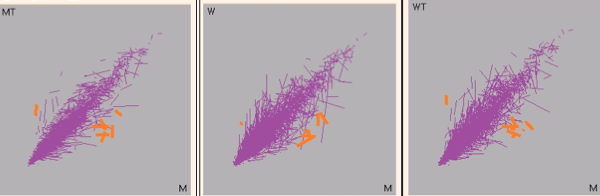
\includegraphics[width=0.8\textwidth]{porcupine}
    \end{framed}
    \caption{Three replicate line plots in which genes of interest (show low variability across replicates but high variability across treatments) are highlighted in orange. For example, in the plot on the left, there are two treatments (MT and M) that each have two replicates. If a gene shows high variability between the two treatments, then it would fall away from the x=y line. If a gene shows low variability between replicates, then the distance between the two replicates will be short. Hence, the genes of interest will be visually represented as the orange ones that are short in length and deviate from the x=y line.}
    \label{fig:porcupine}
\end{figure}

We demonstrate our new interactive litre plots in Chapter~\ref{sec:chapter2} using real RNA-sequencing data. We then demonstrate them again in Chapter~\ref{sec:chapter4} as part of our study of virus and diet quality effects on honey bee gene expression. This later example demonstrates how we updated and expanded the use of these plots to accommodate a situation where there are up to 12 replicates.

\end{enumerate}

%%%%%%%%%%%%%%%%%%%%%%%%%%%%%%%%%%%%%%%%%%%%%%%%%%%%%%%%%%%%%%%%%%%
%%%%%%%%%%%%%%%%%%%%%%%%%%%%%%%%%%%%%%%%%%%%%%%%%%%%%%%%%%%%%%%%%%%

\section{Literature review}
\label{sec:litReview}
%%%%%%%%%%%%%%%%%%%%%%%%%%%%%%%%%%%%%%%%%%%%%%%%%%%%%%%%%%%%%%%%%%%
\subsection{Visualization methods for genealogical data}

Publishing in the open source \pkg{R} statistical programming language allows for tools to be distributed and modified at ease, encourages cross-platform collaboration, and provides a foundation for effective and aesthetic data visualization from the grammar of graphics. There are several useful \pkg{R} packages that offer tools for analyzing and visualizing genealogical datasets. Here, we introduce these packages, and emphasize the shortcomings for which our package \pkg{ggenealogy} brings to this collection of work.

The \pkg{R} package \pkg{pedigree} is named after the standardized chart used to study human family lines, and sometimes used to select breeding of animals, such as show dogs (\citealt{ped}). This package does provide tools that perform methods on parent-child datasets, such as rapidly determining the generation count for each member in the pedigree. However, it does not provide any visualization tools.

Another \pkg{R} package called \pkg{kinship2} does produce basic pedigree charts (\citealt{kin}). In Figure \ref{fig:kinshipFig}, we provide an example pedigree chart from the \pkg{kinship2} package vignette. This pedigree chart adheres to the standard set of symbols used for visualizing genealogical structures: Males are represented with squares and females with circles. Parents are connected to each other by horizontal lines, and to their children by vertical lines. Siblings are connected by horizontal sibship lines. Even though this standard pedigree chart creates powerful charts that can be applied across many applications, it cannot provide unequivocal information in situations where inter-generational breeding occurs, as is often the case in agronomic genealogical lineages.

We demonstrate how the standardized pedigree charts in the \pkg{kinship2} package generate ambiguous results in such scenarios by superimposing a hypothetical inter-generational breeding case in Figure \ref{fig:kinshipFig}. In that figure, each generation is defined by its position on the vertical axis, with the first generation containing individuals 201 and 202. We superimposed green-highlighted individual 215 onto the pedigree chart for explanatory purposes. Its parents are individuals 201 and 206, which are from generations one and two, respectively, and have a parent-child relationship between themselves. As an offspring of a parent-child relationship, individual 215 is both a second and third generation individual. Hence, individual 215 should be displayed in both second and third generational positions on the vertical axis. However, standard pedigree tools only allow for an individual to be displayed once. As a result, in special cases where inter-generational breading occurs, such as in agronomic applications, standardized tools for visualizing genealogical information ambiguously portray the genealogical dataset.

\begin{figure}[H]
    \begin{framed}
    \centering
    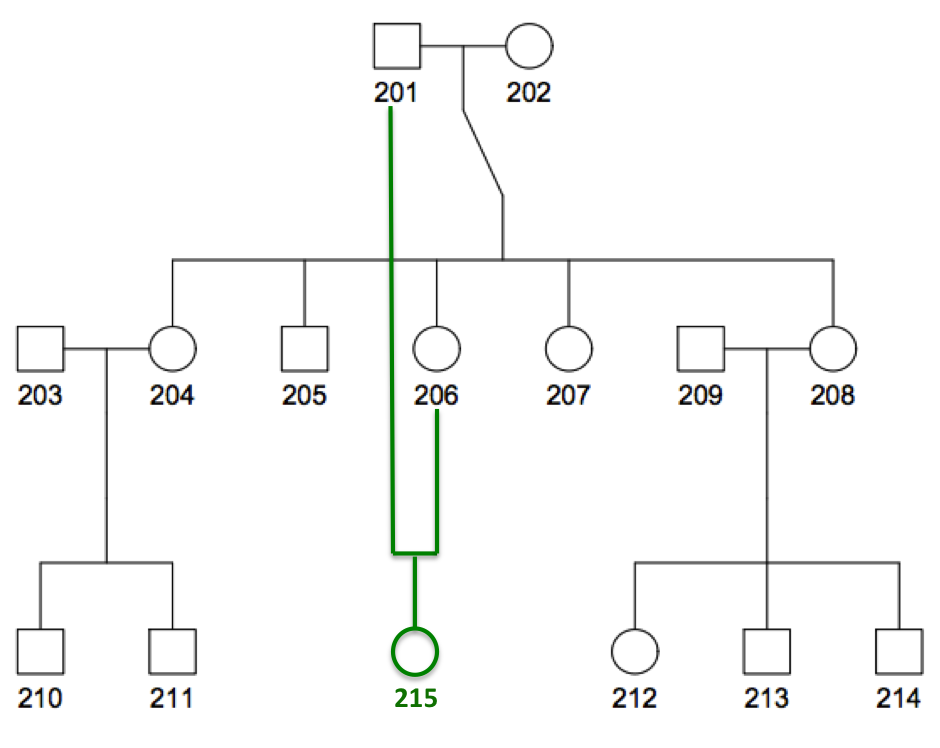
\includegraphics[width=0.65\textwidth]{kinshipFig}
    \end{framed}
    \caption{Example pedigree chart from the \pkg{kinship2} package, where the vertical axis denotes generation count. We superimposed green-highlighted individual 215 for explanatory purposes. As an offspring of a parent-child relationship, individual 215 is both a second and third generation individual. Hence, it should be displayed twice on the vertical axis, once for each of its generation counts. However, standard pedigree tools only allow for an individual to be displayed once, leading to ambiguous portrayal of the genealogical dataset.}
    \label{fig:kinshipFig}
\end{figure}

In addition, popular graph drawing software such as \pkg{GraphViz} and \pkg{Cytoscape} can be used to visualize genealogical structures (\citealt{graphvizCit}, \citealt{cytoscapeCit}). Graphs are defined as objects with sets of nodes and edges, where sets indicate that their comprised elements cannot be repeated. In other words, graphical structures do not allow for repeated nodes, and hence, as is the case with the aforementioned \pkg{R} packages, these popular graph plotting software cannot precisely portray the genealogical dataset in cases of inter-generational breeding.

We again illustrate this problem in Figure \ref{fig:Graph} with an example genealogy using popular graph drawing software like \pkg{GraphViz} and \pkg{Cytoscape}. Here, generation count is denoted by the vertical axis. As was shown in Figure \ref{fig:kinshipFig}, here too we superimpose a green node that has parents from two different generations. This green node is both a second and third generation individual, and should be displayed in both corresponding generation positions on the vertical axis. However, standard graph visualization tools only allow for a given node to be displayed once. As a result, this green node must be ambiguously positioned in either the second or third generation position; in the figure, it is denoted as a third generation individual. In Chapter~\ref{sec:chapter1}, we will demonstrate \pkg{ggenealogy} plots that can remedy these problems.

\begin{figure}[H]
    \begin{framed}
    \centering
    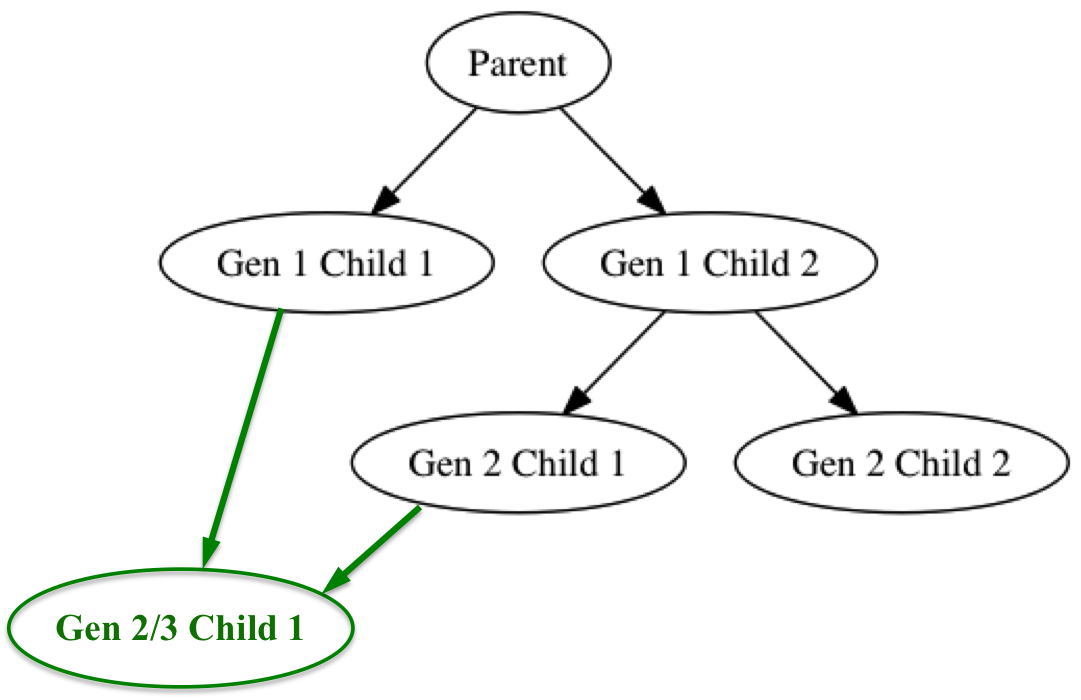
\includegraphics[width=0.6\textwidth]{Graph}
    \end{framed}
    \caption{Example genealogical display using popular graph software like \pkg{GraphViz} and \pkg{Cytoscape}, with generation count denoted by the vertical axis. As was shown in Figure \ref{fig:kinshipFig}, the green node has parents from two different generations, and hence must be ambiguously positioned as one of two generation counts.}
    \label{fig:Graph}
\end{figure}

%%%%%%%%%%%%%%%%%%%%%%%%%%%%%%%%%%%%%%%%%%%%%%%%%%%%%%%%%%%%%%%%%%%
\subsection{Visualization methods for RNA-sequencing data}

Previous studies have provided sound evidence that gene expression data is most effectively explored by using graphical and numerical approaches in a complementary fashion (\citealt{extra2}, \citealt{extra1}, \citealt{extra4}). The authors of one study demonstrated this finding by applying modeling and visualization tools to simulated and real microarray data (\citealt{jds}). Through the use of plots, they determined that their initial models were inappropriate and needed improvement, and that the data quality was questionable and needed relabeling.

Moreover, they demonstrated that some of the most common plots for gene expression data are rife with problems, while some of the less popular plots are useful. In one example, they showed that heat maps are commonly-used, but they do not allow users to detect outlying genes. In contrast, scatterplots can allow for outlier detection. Furthermore, they introduced a new type of plot called the replicate line plot, which can be used to visually mine for genes that show low variability in read counts between replicates but high variability in read counts between treatments. The authors also showed the importance of interaction on plots for gene expression analysis; they used GGobi (\citealt{ggobi}, \citealt{ggobi2}, \citealt{ggobi3}) to generate direct manipulation and linking between various multivariate plots to display the data. Interactive plots for multivariate data could also be accomplished with the use of projections (\citealt{extra3}).

Despite the availability of many ready-made testing software, reliable detection of differentially expressed genes (DEGs) in RNA-sequencing data is not a trivial task. While the data collection might be considered high-throughput, data analysis has intricacies that require careful human attention. In light of this, researchers should use effective and modern data analysis techniques, and verify and enhance the appropriateness of their models with visual feedback. There is a need to make it easier for researchers to use models and visuals in a complimentary fashion during RNA-seq data analysis.

%%%%%%%%%%%%%%%%%%%%%%%%%%%%%%%%%%%%%%%%%%%%%%%%%%%%%%%%%%%%%%%%%%%
%%%%%%%%%%%%%%%%%%%%%%%%%%%%%%%%%%%%%%%%%%%%%%%%%%%%%%%%%%%%%%%%%%%
\section{Overview of thesis research}

%%%%%%%%%%%%%%%%%%%%%%%%%%%%%%%%%%%%%%%%%%%%%%%%%%%%%%%%%%%%%%%%%%%

In chapter~\ref{sec:chapter1}, we introduce \textbf{\pkg{ggenealogy}} (\citealt{ggen}), a published \pkg{R} software package that provides tools for searching through genealogical data, generating basic statistics on their graphical structures using parent and child connections, and displaying the results. The package allows users to draw the genealogy in relation to variables related to the nodes, and to determine and display the shortest path distances between the nodes. Production of pairwise distance matrices and genealogical diagrams constrained on generation are also available in the visualization toolkit. We have tested the tools on a dataset with milestone cultivars of soybean varieties (\citealt{soybean}) as well as on a web-based database of the academic genealogy of mathematicians (\citealt{mgp}).

Susan VanderPlas began the original work for this package and developed most features in the \code{plotAncDes()} function. The software package has been available on the Comprehensive \pkg{R} Archive Network since March 2015 (\citealt{ggen}). In August 2015, a paper introducing the \pkg{ggenealogy} software package received a student paper competition award from the Statistical Computing and Graphics Section of the American Statistical Association. Our paper describing the software package has been accepted to the Journal of Statistical Software. In Decemer 2016, we released a second version of the package as we have added interactive plotting tools that were not available in the first version.

In chapter~\ref{sec:chapter2}, we use several public RNA-sequencing data sets to show that our visualization tools can detect normalization issues, DEG designation problems, and common analysis errors. We also show that our visual tools can identify genes of interest in ways undetectable with models. In this chapter, we propose that users slightly modify their approach to RNA-seq analysis by incorporating statistical graphics into their usual analysis pipelines. Specifically, we emphasize the use of scatterplot matrices, litre plots, and parallel coordinate plots.

In chapter~\ref{sec:chapter3}, we introduce \textbf{\pkg{bigPint}}, a software package we aim to publish on Bioconductor that provides the tools we demonstrated to be useful for RNA-seqeuncing analysis through extensive case studies in chapter~\ref{sec:chapter2}. Namely, the package provides users with easy-to-use methods to create scatterplot matrices, litre plots, and parallel coordinate plots, both in static and interactive formats. We discuss the technology behind creating the interactive features of our graphic techniques, including some of their unique capabilities to plot interactive foreground datasets onto static background datasets. Some of the interactive graphics are shown already as Shiny application links in chapter~\ref{sec:chapter2}. However, we also show new examples in chapter~\ref{sec:chapter3}. We briefly discuss the reference manual and how our software methods can be easily incorporable into popular RNA-sequencing analysis software (\citealt{deseq2}, \citealt{edger}, \citealt{limma}).

In chapter~\ref{sec:chapter4}, we conduct a RNA-sequencing study on the effects of viral innoculation and diet quality on honey bee gene expression. Adam Dolezal began the original work and collected the bee mortality and physical data. We found that the diet quality effect had a much large transcriptomic response than the viral effect in terms of the number of DEGs. We also performed extensive visualization analysis methods using the graphics we developed and introduced in chapters~\ref{sec:chapter2} and ~\ref{sec:chapter3}. Through this process, we discovered that the data and even the DEGs did not appear clean in terms of replicate consistency and treatment differentiation. We compared our study to another study that also investigated the honey bee transcriptomic response to viral innoculation only it used honey bees that had 75\% genetic similarity as opposed to our honey bees that had 25\% genetic similarity (\citealt{galbraith}). We visually confirmed that their data and DEGs appeared much cleaner. By verifying the subsantial overlap in the DEG lists between our study and their study, we were able to place much higher confidence in the DEG results from our otherwise noisy data.

%%%%%%%%%%%%@@@@%%%%%%%%%%%%%%%%%%%%%% CHAPTER %%%%%%%%%%%%%%%%%%%%%%%%%%%%%%%%%%%%%% 
%%%%%%%%%%%%%%%%%%%%%%%%%%%%%%%%%%%%%%%%%%%%%%%%%%%%%%%%%%%%%%%%%%%%%%%%%%%%%%%%%%%%%  
 
\chapter{Visualization methods for genealogical datasets}
\label{sec:chapter1}

\section{Introduction}

Genealogy is the study of parent-child relationships. By tracing through parent-child lineages, genealogists can study the histories of features that have been modified over time. Comparative geneticists, computational biologists, and bioinformaticians commonly use genealogical tools to better understand the histories of novel traits arising across biological lineages. For example, desirable modifications in crops could include an increase in protein yield or an increase in disease resistance, and genealogical structures could be used to assess how these desirable traits developed. At the same time, genealogical lineages can also be used to assess detrimental features, such as to determine the origin of hazardous traits in rapidly-evolving viruses.

Genealogical structures can also serve as informative tools outside of a strict biological sense. For instance, we can trace mentoring relationships between students and dissertation supervisors with the use of academic genealogies. This can allow us to understand the position of one member in the larger historical picture of academia, and to accurately preserve past relationships for the knowledge of future generations. Similarly, linguistic genealogies can be used to decipher the historical changes of vocabulary and grammatical features across related languages. In short, there is a diverse array of disciplines that can elicit useful information about features of interest by using genealogical data.

In all these examples, the genealogical relationships can be represented visually. Access to various types of plotting tools can allow scientists and others to more efficiently and accurately explore features of interest across the genealogy. We introduce here a developing visualization toolkit that is intended to assist users in their exploration and analysis of genealogical structures. In this paper, we demonstrate the main tools of the software package \pkg{ggenealogy} using two example genealogical datasets, one of soybean cultivars (\citealt{soybean}) and the other of academic mathematicians (\citealt{mgp}).

\section{Example datasets}
\label{exData}

The \pkg{ggenealogy} package comes with two example datasets, one comprises a soybean genealogy and the other comprises an academic statistician genealogy. We will introduce both example datasets to demonstrate some of the tools available in the software.

\subsection{Soybean genealogy}

We start with the soybean genealogy, which is available as a data frame structure with 390 rows and five columns. These data were collected from field trials, genetic studies, and United States Department of Agriculture (USDA) bulletins, and date as early as the first decade of the 1900s. They contain information on the copy number variants, single nucleotide polymorphisms, and protein content for each of the varieties, although we removed that information for a succinct example dataset. In this context, the software could ideally be used by agronomists who wish to study how soybean varieties are related. By referencing the visualization of the genealogical structure, these scientists may better understand genetic testing results - in this particular dataset, in terms of copy number variants, single nucleotide polymorphisms, protein content, and yield - and use that knowledge in future breeding decisions.

Each row contains information about a particular child soybean variety, including the name of the child, its yield, the year it was released, whether or not its release year was imputed, and the name of its parent. It should be noted that it typically requires many crosses over the span of one to two decades to develop a new variety that has introduced a desired trait and/or removed an undesired trait. Hence, the release year variable in this dataset represents the year in which the variety was released to the public after its development period. While the name of the child is required, the other four columns can have missing values (which are represented in \pkg{R} with the symbol NA for "not available"). As a result, while each row does contain information about a particular child soybean variety, whether or not a given row also contains information about a parent-child relationship between a pair of soybeans depends on whether or not the parent column has a missing value.

In total, there are 230 soybean varieties in the dataset, 206 of which are children and 165 of which are parents. There are soybeans that are both children and parents. Of the children, 156 have two parents, 28 have one parent, and 22 have zero parents. There are 340 parent-child relationships in the dataset.

We can load the example dataset of soybean genealogy (\code{sbGeneal}) and examine its structure. 

\mybox{
\texttt{R> install.packages("ggenealogy")}\\
\texttt{R> library("ggenealogy")}\\
\texttt{R> data(sbGeneal)}\\
\texttt{R> str(sbGeneal)}
}

\mybox[green!10]{
\texttt{'data.frame':	390 obs. of  5 variables:}\\
\texttt{\$ child       : chr  "5601T" "Adams" "A.K." "A.K. (Harrow)" ...}\\
\texttt{\$ year        : num  1981 1948 1910 1912 1968 ...}\\
\texttt{\$ yield       : int  NA 2734 NA 2665 NA 2981 2887 2817 NA NA ...}\\
\texttt{\$ year.imputed: logi  TRUE FALSE TRUE FALSE FALSE FALSE ...}\\
\texttt{\$ parent      : chr  "Hutcheson" "Dunfield" NA "A.K." ...}
}

\subsection{Academic genealogy of statisticians}

The \pkg{ggenealogy} package also comes with an academic genealogy of statisticians; this dataset is in the form of a data frame with 8165 rows and six columns. To develop this later dataset, we contacted the Math Genealogy Project (\citealt{mgp}), a web-based database for the genealogy of academic mathematicians. This database, which currently contains almost 200,000 entries, is a service of the North Dakota State University Department of Mathematics and the American Mathematical Society. The Mathematics Genealogy Project contact provided us a Structured Query Language (SQL) export, and we used PostgreSQL to query the database (\citealt{psql}).

Each entry in the database contained 26 variables pertaining to an individual who received a graduate-level academic degree in mathematics. One of these variables was called "msc" (Mathematics Subject Classification), and we selected only those entries that contained a value of 62 for this variable (coded as "Statistics"). Furthermore, we only retained entries that had a parent if that parent was also in the field of "Statistics". Hence, in our parent-child relationships, both the child and the parent received postbaccalaureate degrees in statistics, and the parent was the academic advisor to the child. This process resulted in 8995 entries, which we reduced to 8165 entries by removing duplicate entries. With the final data frame of 8165 entries, we only maintained six of the original 26 variables. 

Each row of the final data frame contains information about a particular child who received a graduate-level academic degree in statistics, including the name of the child, the year the child obtained the degree, the country and school from which the child obtained the degree, the thesis title of the degree awarded to the child, and the name of its parent. There are no missing values for the country and school from which the child received its degree or the name of the child; however, some of the years contain missing values (NA), and some of the parent and thesis names contain empty strings (""). As a result, while each row does contain information about a particular child, whether or not a row also contains information about a parent-child relationship between a pair of academic statisticians depends on whether or not the parent column has an empty string.
 
In total, there are 7122 individuals in the dataset, 7122 of which are children and 872 of which are parents. Every parent is also a child, but not every child is also a parent. Of the children, two have four parents, ten have three parents, 226 have two parents, 2801 have one parent, and 4083 have no parents. There are 3291 parent-child relationships in the dataset.

We can load the example dataset of academic genealogy of statisticians (\code{statGeneal}) and examine its structure. 

\mybox{
\texttt{R> data(statGeneal)}\\
\texttt{R> dim(statGeneal)}
}

\mybox[green!10]{
\texttt{[1] 8165    6}
}

\mybox{
\texttt{R> colnames(statGeneal)}
}

\mybox[green!10]{
\texttt{[1] "child"   "parent"  "year"    "country" "school"  "thesis"}
}

\section{Genealogical input format}

As is the case with both example data files introduced above, \pkg{ggenealogy} requires that the genealogy input file is a data frame structure with at least two columns. One column must be labeled "child", and each case in that column must be of type character. The other column must be labeled "parent," and each case in that column must either be of type character, type NA, or type "". At this point, any \pkg{ggenealogy} plot that only requires information about parent-child relationships can be used.

However, some \pkg{ggenealogy} plots also make use of quantitative variable values associated with individuals in the genealogy. For these plots, the input data frame should also contain a third column. In both example data files, this column is labeled "year," and each case in that column can either be of type numeric, type NA, or type "". At this point, any \pkg{ggenealogy} plot can be used.

\section{Generating a graphical object}

Most functions in the \pkg{ggenealogy} software package require an input parameter of a graph structure. Therefore, as a preprocessing step, we must first convert our original data frame structure into a graph structure. Below, we read in the \pkg{R} data file \code{sbGeneal} that is included in the package as a sample data set of soybean genealogy.

We now convert it into an \pkg{igraph} object (\citealt{igraph}) \code{sbIG} using the function \code{dfToIG()}.

\mybox{
\texttt{R> sbIG <- dfToIG(sbGeneal)}\\
\texttt{R> sbIG}
}

\mybox[green!10]{
\texttt{IGRAPH UNW- 230 340 -- }\\
\texttt{+ attr: name (v/c), weight (e/n)}\\
\texttt{+ edges (vertex names):}\\
\texttt{ [1] 5601T    --Hutcheson        Adams    --Dunfield} \\       
\texttt{ [3] A.K.     --A.K. (Harrow)    Altona   --Flambeau} \\       
\texttt{ [5] Amcor    --Amsoy 71         Adams    --Amsoy } \\         
\texttt{ [7] Amsoy 71 --C1253            Anderson --Lincoln   } \\     
\texttt{ [9] Bay      --York             Bedford  --Forrest  }\\       
\texttt{[11] Beeson   --Kent             Blackhawk--Richland } \\      
\texttt{[13] Bonus    --C1266R           Bradley  --J74-39  } \\       
\texttt{[15] Bragg    --Jackson          Bragg    --Bragg x D60-7965}\\
\texttt{+ ... omitted several edges}
}

There are many statistics about the \code{sbGeneal} dataset that we may wish to know that cannot easily be obtained through images and tables. The package function \code{getBasicStatistics()} can be called, using the \code{sbIG} object as input. This will return a list of common graph theoretical measurements regarding the genealogical structure. For instance, is the whole structure connected? If not, how many separated components does it contain? In addition to these statistics, the \code{getBasicStatistics()} function will also return the number of nodes, the number of edges, the average path length, the graph diameter, and other graph theoretical information.

\mybox{
\texttt{R> getBasicStatistics(sbIG)}
}

\mybox[green!10]{
\texttt{\$isConnected}\\
\texttt{[1] FALSE}\\

\texttt{\$numComponents}\\
\texttt{[1] 11}\\

\texttt{\$avePathLength}\\
\texttt{[1] 5.333746}\\

\texttt{\$graphDiameter}\\
\texttt{[1] 13}\\

\texttt{\$numNodes}\\
\texttt{[1] 230}\\

\texttt{\$numEdges}\\
\texttt{[1] 340}\\

\texttt{\$logN}\\
\texttt{[1] 5.438079}
}

\section{Plotting a shortest path}

With soybean lineages, it may be useful for soybean breeders to track how two varieties are related to each other via parent-child relationships. Then, any dramatic changes in yield and other measures of interest between the two varieties can be traced across their genetic timeline. The \pkg{ggenealogy} package allows users to select two varieties of interest, and determine the shortest pathway of parent-child relationships between them, using the \code{getPath()} function. This will return a list that contains the variety names and their years in the path.

\mybox{
\texttt{R> pathTN <- getPath("Tokyo", "Narow", sbIG, sbGeneal)}\\
\texttt{R> pathTN}
}

\mybox[green!10]{
\texttt{\$pathVertices}\\
\texttt{[1] "Tokyo"    "Volstate" "Jackson"  "R66-873"  "Narow"}\\   

\texttt{\$yearVertices}\\
\texttt{[1] "1907"   "1942"   "1954.5" "1971.5" "1985"}
}

The returned path object can then be plotted using the \code{plotPath()} function.

\mybox{
\texttt{R> plotPath(pathTN)}
}

\begin{figure}[h]
    \begin{framed}
    \centering
    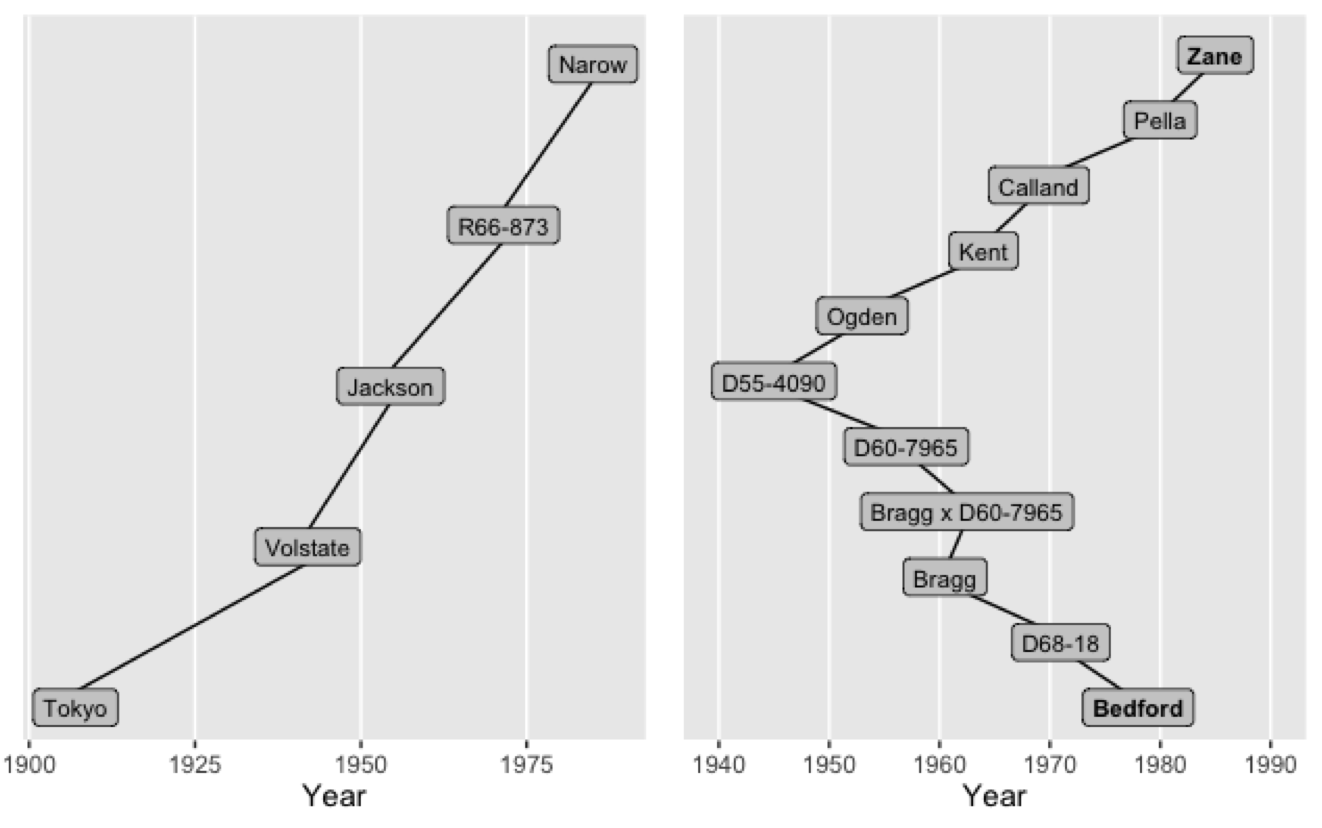
\includegraphics[width=\textwidth]{pathTNZB}
    \end{framed}
    \caption{Left: The shortest path between varieties Tokyo and Narow is strictly composed of a unidirectional sequence of parent-child relationships. Right: The shortest path between varieties Zane and Bedford is not strictly composed of unidirectional parent-child relationships; they instead have a cousin-like relationship.}
    \label{fig:pathTNZB}
\end{figure}

This produces a visual that informs users of all the varieties involved in the shortest path between the two varieties of interest (see left half of Figure \ref{fig:pathTNZB}). In this plot, the release year of all varieties involved in the path are indicated on the horizontal axis, while the vertical axis has no meaning other than to simply to display the labels evenly spaced vertically. The shortest path between varieties \code{Tokyo} and \code{Narow} is composed of a unidirectional series of parent-child relationships, with \code{Tokyo} as the starting ancestor in the early 1900s, \code{Narow} as the most recent descendent in the mid 1980s, and three varieties in between.

Next, we can run the same set of functions on a different pair of varieties. First, a call to the \pkg{ggenealogy} function \code{getYear()} indicates that variety \code{Bedford} was released in 1978 and variety \code{Zane} in 1985.

\mybox{
\texttt{R> getYear("Bedford", sbGeneal)}
}

\mybox[green!10]{
\texttt{[1] 1978}
}

\mybox{
\texttt{R> getYear("Zane", sbGeneal)}
}

\mybox[green!10]{
\texttt{[1] 1985}
}

We can then create a plot showing the shortest path between these two varieties of interest. As this is a longer path, we may also consider setting the \code{fontFace} variable of the \code{plotPath()} to a value of 2, indicating we wish to boldface the two varieties of interest.

\mybox{
\texttt{R> pathBZ <- getPath("Bedford", "Zane", sbIG, sbGeneal)}\\
\texttt{R> plotPath(pathBZ, fontFace = 2)}
}

The resulting plot (right half of Figure \ref{fig:pathTNZB}) allows us to quickly determine that \code{Bedford} is not a parent, grandparent, or any great grandparent of \code{Zane}. Instead, we see that these two varieties are not related through a unidirectional parent-child lineage, but instead have a cousin-like relationship. The oldest common ancestor between \code{Zane} and \code{Bedford} is the variety \code{D55-4090}, which was released in the mid 1940s.

Furthermore, as determined by the figure, for both \code{Zane} and \code{Bedford}, there are four varieties of unidirectional parent-child relationships between each of them and their common ancestor \code{D55-4090}. Hence, any feature of interest that differentiates \code{Zane} and \code{Bedford} (protein content, yield, disease resistance, etc.) can also be examined across these two separate lineage histories.

\section{Superimposing shortest path on tree}

Now that we can create path objects, we may wish to know how those paths are positioned compared to the entire genealogical lineage. For instance, of the documented soybean cultivar lineage varieties, where does the shortest path between two varieties of interest exist? Are these two varieties older compared to the overall data structure? Are they newer? Or, do they span the entire structure, and represent two extreme ends of documented time points?

There is a function available in the \pkg{ggenealogy} package \code{plotPathOnAll()} that can allow users to quickly visualize their path of interest superimposed over all varieties and edges present in the whole data structure. Here we will produce a plot of the shortest path between varieties \code{Tokyo} and \code{Narow} across the entire dataset, as is displayed in Figure \ref{fig:plotTNBin3}.

\mybox{
\texttt{R> plotPathOnAll(pathTN, sbGeneal, sbIG, binVector = 1:3, pathEdgeCol = "red", nodeSize = 2.5, pathNodeSize = 4) + ggplot2::theme(axis.text = ggplot2::element\_text(size = 12), axis.title = ggplot2::element\_text(size = 12))}
}

\begin{figure}%[h]
    \begin{framed}
    \centering
    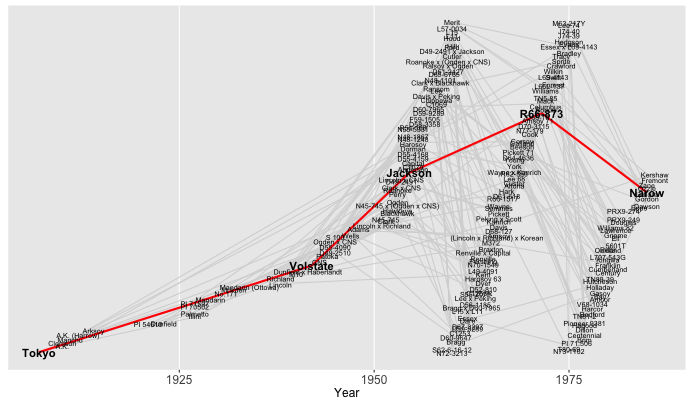
\includegraphics[width=\textwidth]{plotTNBin3}
    \end{framed}
    \caption{The shortest path between Tokyo and Narow, superimposed over the data structure, using a bin size of 3.}
    \label{fig:plotTNBin3}
\end{figure}

In the code above, syntax from the \pkg{ggplot2} package was appended to the \code{plotPathOnAll()} function; this can be done for most \pkg{ggenealogy} functions (\citealt{ggplot2}). While the first three explicit parameters have been introduced earlier in this paper, the fourth parameter (\code{binVector}) requires some explanation. The motivation of the \code{plotPathOnAll()} function is to write node labels on a plot, with the center of each node label constricted on the horizontal axis to its quantitative variable of interest (in this case, year of release). As is the case for the plots before, the vertical axis has no meaning other than providing a plotting area in which to draw the node labels. Unfortunately, for large datasets, this motivation can be a difficult task because the text labels of the varieties can overlap if they are assigned a similar y coordinate, have a similar year (x coordinate), and have long text labels (width of x coordinate).

For each variety, the x coordinate (year) and width of the x coordinate (text label width) cannot be altered, as they provide useful information. However, for each variety, the y coordinate is arbitrary. Hence, in an attempt to mitigate text overlapping, the \code{plotPathOnAll()} function does not randomly assign the y coordinate. Instead, it allows users to partially control the y coordinates with a user-determined number of bins (\code{binVector}).

If the user decides to produce a plot using three bins, as in the example code above, then the varieties are all grouped into three bins based on their year values. In other words, there will be bin 1 (the "oldest bin") which includes the one-third of varieties with the oldest years of release, bin 2 (the "middle bin"), and bin 3 (the "youngest bin"). Then, in order to decrease text overlap, the consecutively increasing y-axis coordinates are alternatively assigned to the three bins (For example: bin 1, bin 2, bin 3, bin 1, bin 2, bin 3, ...) repeatedly until all varieties are addressed. This algorithm means that for any pair of varieties within a given bin, there are exactly two other varieties vertically separating them.

In the code above, \code{binVector} was assigned a value of 3, and \code{pathEdgeCol} was assigned a value of "red". Additionally, we specified a size of 2.5 for the non-path node test using the \code{nodeSize} parameter, and a size of 4 for the path node text using the \code{pathNodeSize} parameter. There are several other parameters in the \code{plotPathOnAll()} function, which can be read in more detail using the help command.

This code resulted in Figure \ref{fig:plotTNBin3}, where we see that edges not on the path of interest are thin and gray by default, whereas edges on the path of interest are bolded by default. We also see that variety labels in the path of interest are boldfaced by default. Figure \ref{fig:plotTNBin3} presents useful information: We immediately gather that the path of interest does span most of the years of the data structure. In fact, \code{Tokyo} appears to be the oldest variety in the dataset, and \code{Narow} appears to be one of the youngest varieties. We can also determine that the majority of varieties were released between 1950 and 1970.

However, Figure \ref{fig:plotTNBin3} has significant empty spaces between the noticeably distinct bins, whereas almost all text labels are overlapping, thereby decreasing their readability. To force text labels into these spaces, the user may consider using a larger number of bins. Hence, we next examine a bin size of 6 to create Figure \ref{fig:plotTNBin6}.

\mybox{
\texttt{R> plotPathOnAll(pathTN, sbGeneal, sbIG, binVector = 1:6, pathEdgeCol = "seagreen2", nodeSize = 1, pathNodeSize = 3)}
}

\clearpage

\begin{figure}[H]
    \begin{framed}
    \centering
    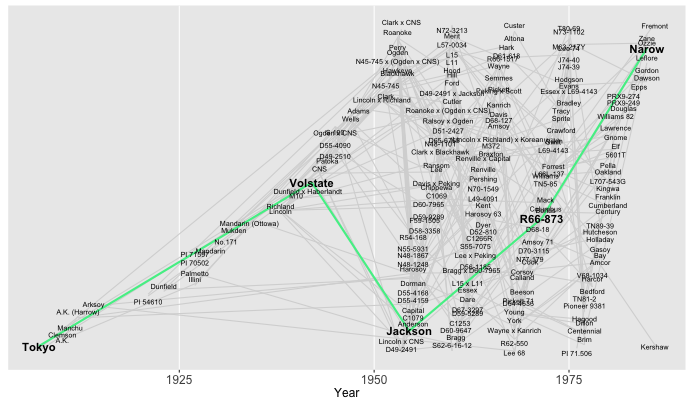
\includegraphics[width=\textwidth]{plotTNBin6}
    \end{framed}
    \caption{The shortest path between Tokyo and Narow, superimposed over the data structure, using a bin size of 6.}
    \label{fig:plotTNBin6}
\end{figure}

We can immediately see that Figure \ref{fig:plotTNBin6} more successfully mitigates text overlap compared to Figure \ref{fig:plotTNBin3}. We can also confirm what we saw in the previous plot that indeed most varieties were released between 1950 and 1970, and any textual overlap is confined to this range of years.

\section{Plotting ancestors and descendants by generation}
\label{remedy}

The most novel visual function in \pkg{ggenealogy}, \code{plotAncDes()} allows users to view the ancestors and descendants of a given variety. The inputted variety is highlighted in the center of the plot, ancestors are displayed to the left of the center, and descendants are displayed to the right of the center. The further from the center that a variety is located, the more generations that variety is distanced from the centered variety of interest.

This particular \pkg{ggenealogy} tool is unique because most available genealogy and graph visualization software do not allow for repeated labels. It is a useful tool because, as was demonstrated in Figures \ref{fig:kinshipFig} and \ref{fig:Graph}, some genealogical datasets require repeated node labels if they are to be visualized by generation counts. Indeed, our example soybean genealogy is one such dataset.

To demonstrate this tool, we will create a plot of the ancestors and descendants of the variety \code{Lee}. We specify that the maximum number of ancestor and descendant generations are both 6, and that the text of the variety of interest is highlighted in blue:

\mybox{
\texttt{R> plotAncDes("Lee", sbGeneal, mAnc = 6, mDes = 6, vCol = "blue")}
}

This generates the top plot of Figure \ref{fig:Lee}. We notice that \code{Lee} has 3 generations of ancestors and 5 generations of descendants. We also notice that some varieties are repeated in the plot, which is a unique feature provided by \pkg{ggenealogy}. For example, the variety \code{5601T} is represented four times - once as a third generation descendant of \code{Lee}, once as a fourth generation descendant of \code{Lee}, and twice as a fifth generation descendant of \code{Lee}. The variety \code{5601T} was repeated multiple times because there are multiple paths between \code{Lee} and \code{5601T}. For explanation purposes, all paths between \code{Lee} and \code{5601T} were manually highlighted in blue.

\begin{figure}[H]
    \begin{framed}
    \centering
    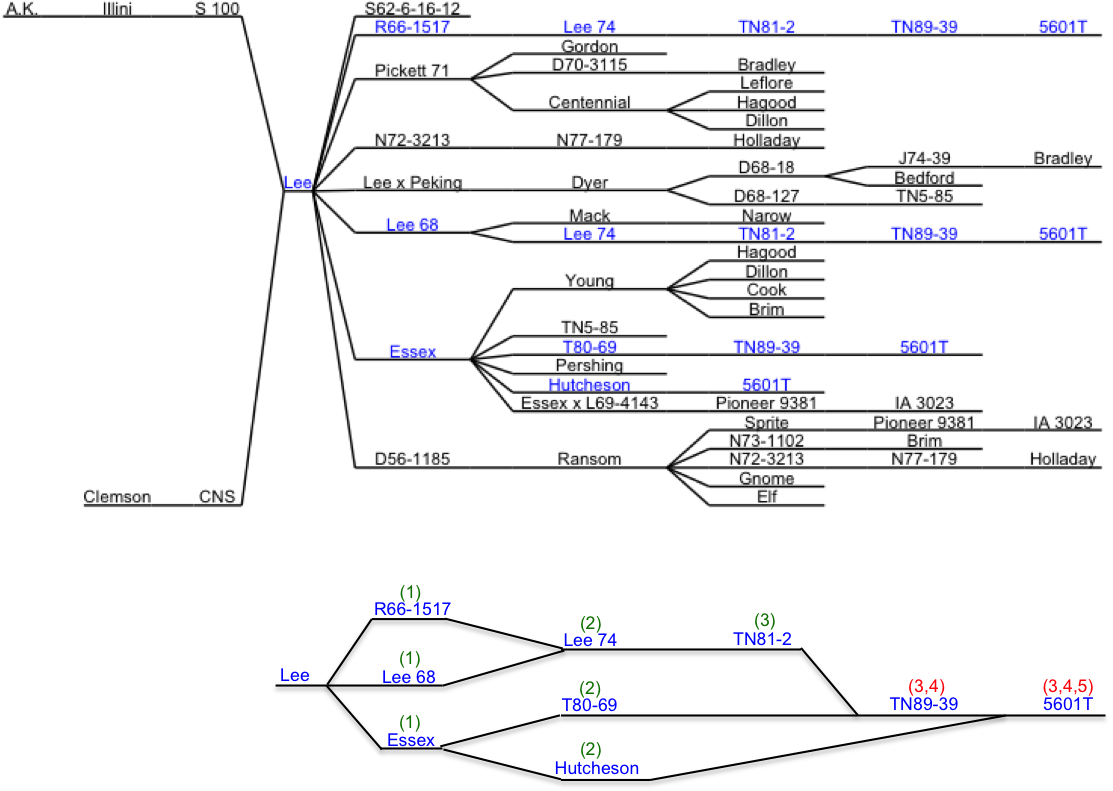
\includegraphics[width=\textwidth]{LeeAD3}
    \end{framed}
    \caption{Top: All ancestors and descendants of the variety Lee are shown in this ggenealogy plot. Bottom: We now attempt to mimic the blue paths in the ggenealogy plot on the top, only now nodes cannot be repeated. The parenthetical numbers above each node represents the set of generation counts that node is away from the center node Lee. The presence of red parentheses indicate that the plot on the bottom ambiguously display the example soybean genealogy in the way that the ggenealogy plot on the top can accomplish.}
    \label{fig:Lee}
\end{figure}

The bottom plot of Figure \ref{fig:Lee} is not an output plot of \pkg{ggenealogy}. Instead, it was simply created for didactic purposes. Here, the paths that were manually highlighted in blue in the top plot produced by \pkg{ggenealogy} are shown again, only now nodes cannot be repeated. The parenthetical number above each node represents the set of generation counts distancing that node from the center node \code{Lee}; green parentheses indicate that the node could be successfully placed in one horizontal position, but red parentheses indicate that the node could not be successfully placed in one horizontal position. We see that node \code{TN89-39} cannot simultaneously be represented as both a third and fourth descendent of node \code{Lee}, and node \code{5601T} cannot simultaneously be represented as a third, fourth, and fifth descendent of node \code{Lee}. Hence, without allowing nodes to repeat, this dataset cannot be presented in the graph on the bottom as it can be in the \pkg{ggenealogy} graph on the top. This is a current limitation in other genealogy and graphical software that \pkg{ggenealogy} can now provide.

\section{Plotting distance matrix}

It may also be of interest to generate matrices where the colors indicates a variable between all pairwise combinations of inputted varieties. The package \pkg{ggenealogy} also provides a function \code{plotDegMatrix()} for that purpose. We can demonstrate this function with the variable being the shortest path degree between a given pair of varieties. The shortest path degree is calculated as the smallest number of parent-child edges needed to traverse between two varieties of interest. For instance, in Figure \ref{fig:pathTNZB}, the shortest path degree between \code{Tokyo} and \code{Narow} is four and the shortest path degree between \code{Bedford} and \code{Zane} is ten.

Here we generate a distance matrix for a set of 10 varieties, setting the x-label and y-label as "Variety" and the legend label as "Degree". In this example, we add \pkg{ggplot2} functionality to specify that pairs with small degrees are white, while those with large degrees are dark green, as well as to specify the text size of the legend title and label.

\mybox{
\texttt{>R varieties <- c("Brim", "Bedford", "Calland", "Dillon", "Hood", "Narow", "Pella", "Tokyo", "Young", "Zane")}\\
\texttt{>R plotDegMatrix(varieties, sbIG, sbGeneal, "Variety", "Variety", "Degree") + ggplot2::scale\_fill\_continuous(low = "white", high = "darkgreen") + ggplot2::theme(legend.title = ggplot2::element\_text(size = 15), legend.text = ggplot2::element\_text(size = 15))}
}

This creates the plot in Figure \ref{fig:degMatrix}. We see that the degree of the shortest path between varieties \code{Bedford} and \code{Zane} is 10, which is consistent with what we saw earlier in Figure \ref{fig:pathTNZB}. However, we now also see that a shortest path degree of 10 may be considered relative to the rest of this dataset.

\begin{figure}[h]
    \begin{framed}
    \centering
    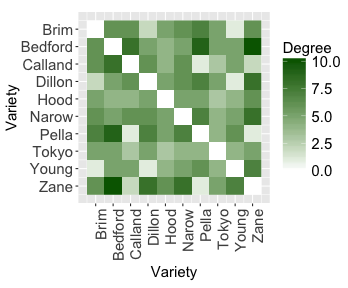
\includegraphics[width=0.5\textwidth]{degMatrix}
    \end{framed}
    \caption{The shortest path degree matrix between ten varieties of interest.}
    \label{fig:degMatrix}
\end{figure}

\section{Academic genealogy of statisticians}

The \pkg{ggenealogy} package comes with two example datasets, and while we have introduced the plant breeding genealogy, we have yet to introduce the academic genealogy. As was demonstrated in Section \ref{exData}, every parent in the academic genealogy is also a child, and some children in the academic genealogy have more than two parents. Neither of these features was the case in the plant breeding genealogy. Additionally, the academic genealogy is much larger than the plant breeding genealogy. Some of these differences may affect how one would approach \pkg{ggenealogy} plotting tools. For this reason, we will now demonstrate some of the \pkg{ggenealogy} plotting tools we already introduced, only now applied to the academic genealogy. 

The ability to plot ancestors and descendants by generation was demonstrated using the plant breeding genealogy in Figure \ref{fig:Lee}. As we believe this is the most novel plotting tool in the \pkg{ggenealogy} package, we will test it again here using the academic genealogy.

We need to choose a central individual of interest in order to create this plot. Perhaps we can use the academic statistician in the dataset that has the largest number of "descendants". To determine the name of this individual, below we use the \pkg{ggenealogy} function \code{getNode()} to create a vector \code{indVec} that contains the names of all individuals in the dataset. We then use the \pkg{dplyr} package to apply the \pkg{ggenealogy} function \code{getDescendants()} on each individual in the \code{indVec} vector (\citealt{dplyr}). We set the parameter \code{gen} to a conservatively large value of 100 as this dataset is unlikely to have any individuals with more than 100 generations of "descendants".

After that, we can generate a table to examine all values of "descendant" counts in the dataset, along with the number of individuals who have each of those values of "descendant" counts. Of the 8165 individuals in this dataset, 6252 of them have zero "descendants", 322 of them have one "descendant", and 145 of them have two "descendants". There are only 17 individuals who have more than 30 "descendants", and there is one individual who has the largest value of 159 "descendants". We determine that this individual is the prominent British statistician Sir David Cox, who is known for the Box-Cox transformation and Cox processes, as well as for mentoring many younger researchers who later became notable statisticians themselves.

\mybox{
\texttt{>R library(dplyr)}\\
\texttt{>R indVec <- getNodes(statGeneal)}\\
\texttt{>R indVec <- indVec[which(indVec != "", )]}\\
\texttt{>R dFunc <- function(var) nrow(getDescendants(var, statGeneal, gen = 100))}\\
\texttt{>R numDesc <- sapply(indVec, dFunc)}\\
\texttt{>R table(numDesc)}
}

\mybox[green!10]{
\texttt{numDesc}\\
\texttt{   0    1    2    3    4    5    6    7    8    9   10   11   12   13   14 }\\
\texttt{6252  322  145   88   58   36   31   22   23   14   17   13   14    9    9 }\\
\texttt{  15   16   17   18   19   20   21   22   23   24   25   26   27   29   30 }\\
\texttt{   6    4    3    2    5    7    5    3    3    2    2    6    1    1    3 }\\
\texttt{  34   37   38   40   41   44   45   48   49   61   62   75   77   84  159 }\\
\texttt{   2    1    1    1    1    1    1    1    2    1    1    1    1    1    1 }
}

\mybox{
\texttt{R> which(numDesc == 159)}
}

\mybox[green!10]{
\texttt{David Cox}\\ 
\texttt{     1980}
}

We can now visualize how these 159 "descendants" are related to Sir David Cox by calling the \code{plotAncDes()} function of \pkg{ggenealogy}, similar to what we did to generate Figure \ref{fig:Lee}. As such, we create Figure \ref{fig:dCox} using the code below.

\mybox{
\texttt{R> plotAncDes("David Cox", statGeneal, mAnc = 6, mDes = 6, vCol = "blue")}
}

\begin{figure}%[h]
    \begin{framed}
    \centering
    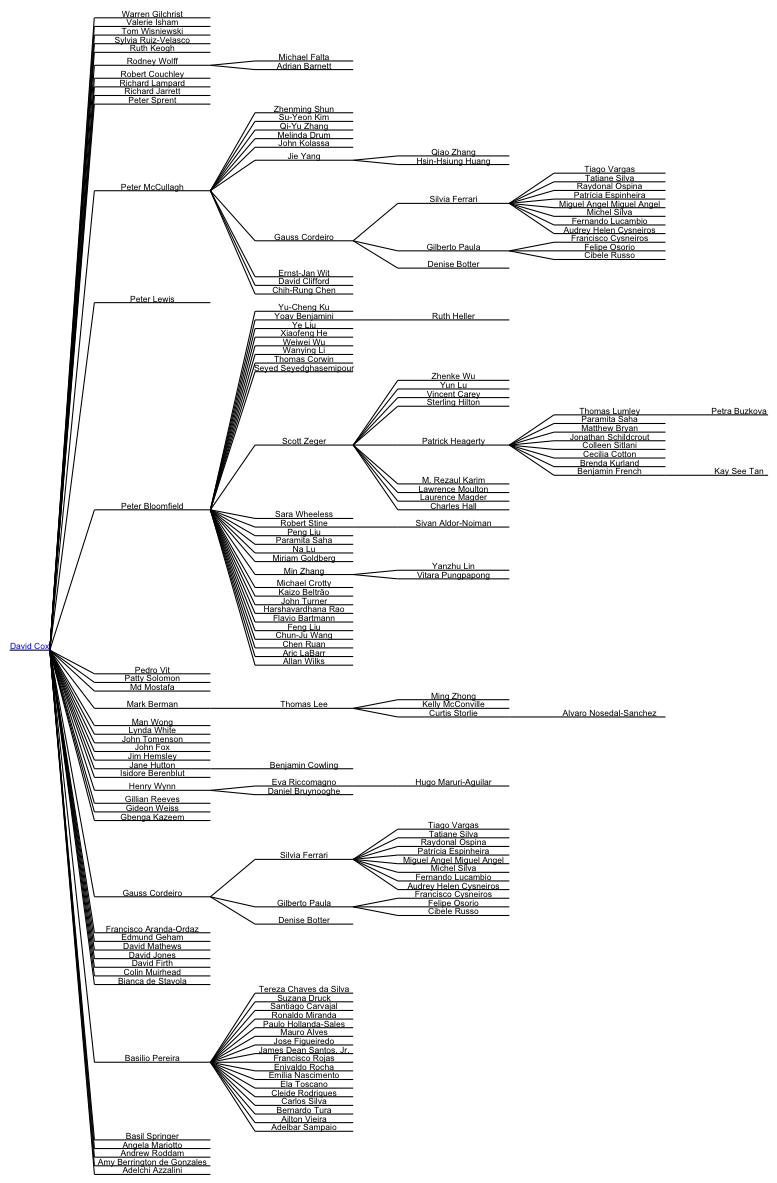
\includegraphics[width=\textwidth]{dCox.png}
    \end{framed}
    \caption{The 159 academic statistician "descendants" of Sir David Cox.}
    \label{fig:dCox}
\end{figure}

We see from Figure \ref{fig:dCox} that Sir David Cox had 42 "children", many of them becoming notable statisticians themselves, such as Basilio Pereira, Valerie Isham, Gauss Cordeiro, Peter McCullagh, and Henry Wynn. Of his "children", the one who produced the most "children" of their own was Peter Bloomfield, who has 26 "children" and 49 "descendants". In total, Sir David Cox had five generations of academic statistics mentees in this dataset.

\mybox{
\texttt{R> length(getChild("Peter Bloomfield", statGeneal))}
}

\mybox[green!10]{
\texttt{[1] 26}
}

\mybox{
\texttt{R> nrow(getDescendants("Peter Bloomfield", statGeneal, gen = 100))}
}

\mybox[green!10]{
\texttt{[1] 49}
}

At this point, it would be insightful to examine a more detailed view of one of the longest strings of "parent-child" relationships between Sir David Cox and one of the two individuals who are his fifth generation "descendants". We do so with the code below, choosing his fifth generation "descendant" to be Petra Buzkova. We set the \code{fontFace} variable of the \code{plotPath()} to a value of 4, indicating we wish to boldface and italicize the two varieties of interest.

\mybox{
\texttt{R> statIG <- dfToIG(statGeneal)}\\
\texttt{R> pathCB <- getPath("David Cox", "Petra Buzkova", statIG, statGeneal, isDirected = FALSE)}\\
\texttt{R> plotPath(pathCB, fontFace = 4) + ggplot2::theme(axis.text = ggplot2::element\_text(size = 10), axis.title = ggplot2::element\_text(size = 10))}
}

\clearpage

\begin{figure}[H]
    \begin{framed}
    \centering
    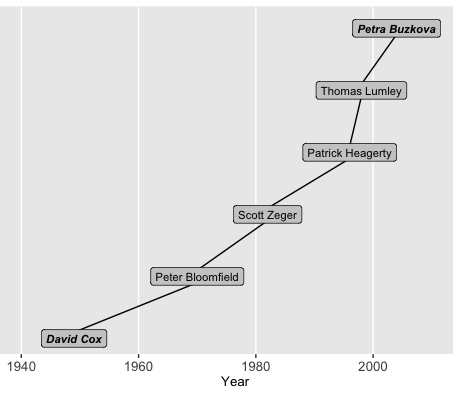
\includegraphics[width=0.7\textwidth]{pathCB}
    \end{framed}
    \caption{The shortest path between Sir David Cox and one of his fifth generation "descendants", Petra Buzkova.}
    \label{fig:pathCB}
\end{figure}

This code results in Figure \ref{fig:pathCB}. We see that the shortest path between Sir David Cox and Petra Buzkova is strictly composed of five unidirectional "parent-child" relationships that span about 55 years. We see that the time difference between when an advisor and student earned their degrees is not consistent across this path: The three statisticians who earned their degrees earliest in this path span more than 30 years in degree acquisition, whereas the three statisticians who earned their degrees later in this path only span less than ten years in degree acquisition.

We also notice in Figure \ref{fig:pathCB} that Sir David Cox received his statistics degree in about 1950, and Petra Buzkova received her statistics degree in about 2005. This genealogy only contains historical information about obtained degrees, and does not project into the future. Hence, we can be assured that Petra Buzkova is one of the younger individuals in the dataset, at least in the sense that the youngest individual could only have received his or her degree ten years after Petra Buzkova. However, we cannot be assured that Sir David Cox is one of the oldest individuals in the dataset. As such, it would be informative to superimpose this path of interest onto the entire dataset, using the \code{plotPathOnAll()} function of the \pkg{ggenealogy} package, as we did for the soybean genealogy in Figures \ref{fig:plotTNBin3} and \ref{fig:plotTNBin6}.

We can achieve this using the below code. After trial and error, we use a \code{binVector} of size 200, and append \pkg{ggplot2} syntax to define suitable x-axis limits. The output of this process is illustrated in Figure \ref{fig:plotCBText}.

\mybox{
\texttt{R> plotPathOnAll(pathCB, statGeneal, statIG, binVector = 1:200) + ggplot2::theme(axis.text = ggplot2::element\_text(size = 8), axis.title = ggplot2::element\_text(size = 8)) + ggplot2::scale\_x\_continuous(expand = c(.1, .2))}
}

\begin{figure}[H]
    \begin{framed}
    \centering
    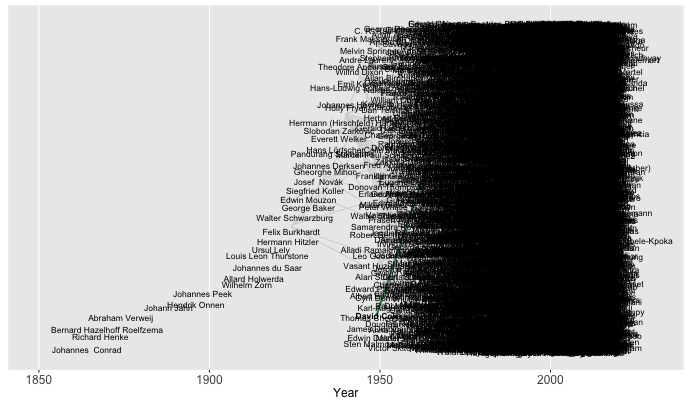
\includegraphics[width=\textwidth]{plotCBText}
    \end{framed}
    \caption{The shortest path between Sir David Cox and Petra Buzkova, superimposed over the data structure, using a bin size of 200.}
    \label{fig:plotCBText}
\end{figure}

We see from the resulting Figure \ref{fig:plotCBText} that almost all text labels for individuals who received their graduate-level statistics degrees between 1950 and 2015 are undecipherable. We also see that the year Sir David Cox acquired his statistics degree is somewhere in the later half of the variable year for this dataset, as the oldest dates for acquisition of statistics degrees in this dataset occur around 1860. However, the number of individuals who are documented as receiving their statistics degrees between 1860 and 1950 are few enough so that their text labels are somewhat readable.

The text labels are so numerous in Figure \ref{fig:plotCBText} that simply trying different values for the input parameter \code{binVector} will not solve the text overlapping problem. Instead, one approach we can try is to reconstruct the plot using the same \pkg{ggenealogy} function \code{plotPathOnAll()}, only now specifying variables to render the size (2.5) and color (default of black) of the text for nodes that are on the path of interest to be more noticeable than the size (0.5) and color (dark gray) of the text for nodes that are not on the path of interest. Moreover, we can make the edges that are not on the path of interest to be represented in a less noticeable color (light gray) than the edges that are on the path of interest (default of dark green). The variable names and options for these aesthetics is further detailed in the help manual of the function. We provide one example code that alters the defaults of the text color and sizes of nodes and edges below, which results in Figure \ref{fig:plotCBNoText}.

\mybox{
\texttt{R> plotPathOnAll(pathCB, statGeneal, statIG, binVector = 1:200, nodeSize = .5, pathNodeSize = 2.5, nodeCol = "darkgray", edgeCol = "lightgray") + ggplot2::theme(axis.text = ggplot2::element\_text(size = 8), axis.title = ggplot2::element\_text(size = 8)) + ggplot2::scale\_x\_continuous(expand = c(.1, .2))}
}

\begin{figure}[H]
    \begin{framed}
    \centering
    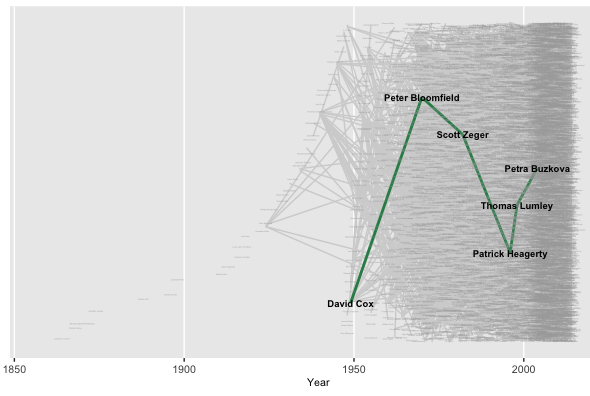
\includegraphics[width=\textwidth]{plotCBNoText}
    \end{framed}
    \caption{The shortest path between Sir David Cox and Petra Buzkova, superimposed over the data structure, using a bin size of 200. Individuals on the shortest path are labeled in large and black text and connected by dark green edges; all other individuals are labeled in small and gray text and connected by light gray edges.}
    \label{fig:plotCBNoText}
\end{figure}

In Figure \ref{fig:plotCBNoText}, we can now see each individual on the path of interest, and how their values for the variable year are overlaid on the entire genealogy structure. We can also more clearly see that, even though only ten years span between the youngest individual in the genealogy and Petra Buzkova, there are many individuals in that last decade. Indeed, the decade from 2005 to 2015 appears to be the densest in this dataset in terms of acquisition of statistics degrees.

\subsection{Interactive visualization of genealogical structure}

We could still improve upon Figure \ref{fig:plotCBNoText}. Even though we may be primarily interested in understanding how the path of interest is overlaid across the entire genealogical structure, we could, upon viewing the entire structure, also develop an interest in nodes that are not on the path of interest but are revealed to stand out among the rest of the genealogical structure. For instance, in Figure \ref{fig:plotCBNoText}, it may be of interest for us to determine the names of the few individuals who obtained their statistics degrees before 1900. Fortunately, within the \code{plotPathOnAll()} function, there is a variable \code{animate} that we can set to a value of TRUE to create an interactive version of the figure that allows us to hover over individual illegible labels and immediately receive their labels in a readable format. A short video demonstration of these interactive features can be viewed upon clicking on Figure \ref{fig:plotAnimate}.

\mybox{
\texttt{R> plotPathOnAll(pathCB, statGeneal, statIG, binVector = 1:200, nodeSize = .5, pathNodeSize = 2.5, nodeCol = "darkgray", edgeCol = "lightgray", animate = TRUE)}
}

\clearpage

\begin{figure}[H]
    \begin{framed}
    \centering
    \includemedia[width=1.0\textwidth, addresource=animateGen.mov, deactivate=onclick, flashvars={source=animateGen.mov}]{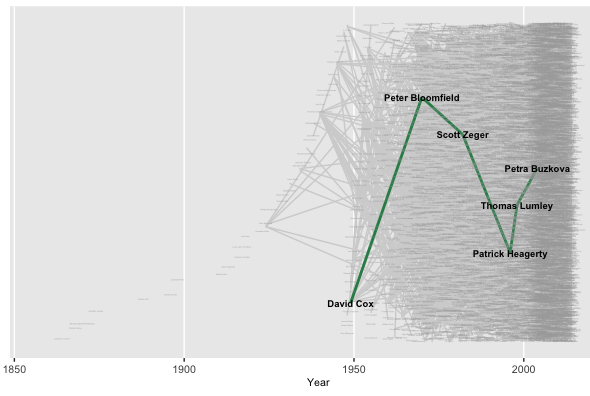
\includegraphics{./plotCBNoText.png}}{VPlayer.swf}
    \end{framed}
    \caption{Upon clicking on this figure twice, a short video demonstrating the animation features for this function can be viewed. Please note that to properly view this video, the PDF version of this paper must be opened in Adobe Acrobat Reader DC (Version >=9), which can be downloaded free of charge.}
    \label{fig:plotAnimate}
\end{figure}

\section{Conclusions}

The \pkg{ggenealogy} package offers various plotting tools that can assist those studying genealogical lineages in the data exploration phases, as well as in preparing publication-suitable images. As each plot comes with its pros and cons, we recommended for users to explore several visualization tools. If users are simultaneously using similar packages, we in particular recommend using the \code{plotAncDes()} function. This plot allows users to view generation counts of a variety of interest in a manner that is not as readily available in similar software packages.

\section{Acknowledgments}

This project was an effort between Susan VanderPlas, Dianne Cook, Michelle A. Graham, and myself. Together, we thank Drs. James E. Specht and Randy C. Shoemaker for helpful discussions of soybean genealogy. In addition, we are grateful for the financial support from the United Soybean Board (Project 1204), The North Central Soybean Research Program, the NSF Plant Genome Research Program (award number 0820642), and the USDA-ARS CRIS Project 3625-21220-005-00D. The USDA is an equal opportunity provider and employer. Mention of trade names or commercial products in this article is solely for the purpose of providing specific information and does not imply recommendation or endorsement by the U.S. Department of Agriculture.


%%%%%%%%%%%%%%%%%@@@@%%%%%%%%%%%%%%%%% CHAPTER %%%%%%%%%%%%%%%%%%%%%%%%%%%%%%%%%%%%%% 
%%%%%%%%%%%%%%%%%%%%%%%%%%%%%%%%%%%%%%%%%%%%%%%%%%%%%%%%%%%%%%%%%%%%%%%%%%%%%%%%%%%%%

\chapter{The case for visualization methods in RNA-sequencing data analysis}
\label{sec:chapter2}

\section{Introduction}

RNA-sequencing (RNA-seq) uses next-generation sequencing (NGS) to estimate the quantity of RNA in biological samples at given timepoints. In recent years, decreasing cost and increasing throughput has rendered RNA-seq an attractive alternative to transcriptome profiling. Prior to RNA-seq, gene expression studies were performed with microarray techniques, which required prior knowledge of reference sequences. RNA-seq does not have this limitation, and has enabled a new range of applications such as transcriptome de novo assembly \citep{Robertson} and detection of alternative splicing processes \citep{Anders2012, Pan}. Coupled with its high resolution and sensitivity, RNA-seq will likely revolutionize our understanding of the intricacies of eukaryotic transcriptomes \citep{Wang, Zhao}.

RNA-seq data is multivariate data, and its basic form is a matrix containing mapped read counts for \textit{n} rows of genes and \textit{p} columns of samples. These mapped read counts provide estimations of the gene expression levels across samples. Researchers typically conduct RNA-seq studies to identify differentially expressed genes (DEGs) between treatment groups. In most popular RNA-seq analysis packages, this objective is approached with models, such as the negative binomial model \citep{Anders2010, Trapnell2012, Trapnell2013, Robinson} and linear regression models \citep{Law}.

Initially, it was widely claimed that RNA-seq produced unbiased data that did not require sophisticated normalization \citep{Wang, Morin, Marioni}. However, numerous studies have since revealed that RNA-seq data is replete with biases and that accurate detection of DEGs is not a negligible task. Problems that complicate the analysis of RNA-seq data include nucleotide and read-position biases \citep{Hansen}, biases related to gene lengths and sequencing depths \citep{Oshlack, RobinsonOshlack}, biases introduced during library preparation \citep{McIntyre}, biases pertaining to the number of replications \citep{Schurch}, biases derived from overlapping sense-antisense transcripts and gene isoforms \citep{Trapnell2013}, and the confounding combination of technical and biological variability \citep{Bullard}.

In light of these complications, researchers should analyze RNA-seq data like they would any other biased multivariate data. Simply applying models to such data is problematic because models hold assumptions that they alone cannot call into question. Fortunately, data visualization enables researchers to see patterns and problems they may not otherwise detect with traditional modeling. As a result, the most effective approach to data analysis is to iterate between models and visuals, and enhance the appropriateness of applied models based on feedback from visuals \citep{Shneiderman}. With RNA-seq data, we primarily want to compare the variability between replicates and between treatment groups. This is visually best achieved by drawing the mapped read count distributions across all genes and samples. Unfortunately, the few plotting tools offered in popular RNA-seq packages do not allow users to effectively view their data in this manner.

In this paper, we strive to remedy this problem by publishing new and effective RNA-seq plotting tools. We use real RNA-seq data to show that our tools can detect normalization problems, DEG designation problems, and common errors in the analysis pipeline. We also show that our tools can identify genes of interest that cannot otherwise be obtained by models. We emphasize that interactive graphics should be an indisposable component of modern RNA-seq analysis: Researchers should be able to quickly flip through plots of genes that appear promising or problematic, and link between plots to swiftly obtain various perspectives of their data. Here, we do not propose that users drastically change their approach to RNA-seq analysis. Instead, we propose that users simply modify their approach to RNA-seq analysis by assessing the sensibility of their models with multivariate graphical tools, namely with parallel coordinate plots, scatterplot matrices, and litre plots.

\section{Parallel Coordinate Plots}

Parallel coordinate plots are essential to visually verify the relationships between variables in multivariate data. A parallel coordinate plot draws each row (gene) as a line. Connections between samples with positive correlations are flat, and connections between samples with negative correlations are crossed. The ideal dataset has more variability between treatments than between replicates. Researchers can quickly confirm this with a parallel coordinate plot: There should be flat connections between replicates but crossed connections between treatments.

There are several packages within the Bioconductor software that provide graphics for RNA-seq data analysis \citep{Huber}. Two of the most common graphic techniques are side-by-side boxplots and Multidimensional Scaling (MDS) plots \citep{Love, Risso, Robinson, Ritchie}. Unfortunately, these plots can hide problems that still exist in the data even after normalization and that could be better detected with parallel coordinate plots.

Figure~\ref{simulatedData} exemplifies this problem for two simulated datasets, one displayed on the left half and the other displayed on the right half of the figure. Each dataset contains two treatment groups (A and B) with three replicates. We cannot detect any notable differences between the left and right datasets from the side-by-side boxplots (subplots A) as they both show fairly consistent five number summaries across their six samples. Likewise, we cannot detect notable differences between the datasets from the MDS plots (subplots B) as they both suggest that the datasets are clustered by the two treatment groups, although the first replicate from treatment A appears as an outlier in the right MDS plot.

\begin{figure}[!tpb]
\begin{framed}
\centerline{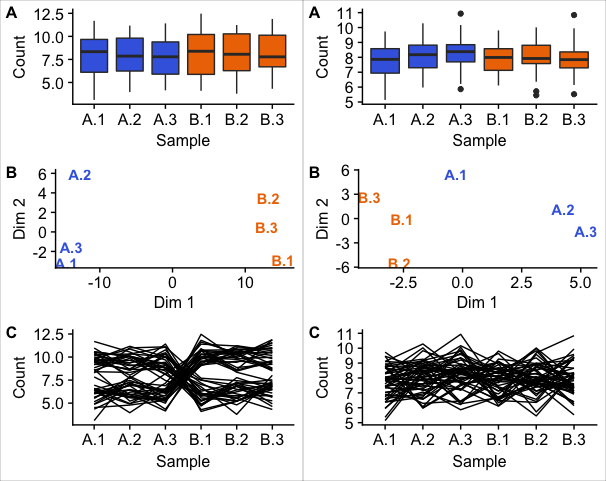
\includegraphics[width=\columnwidth]{MakeFigures/simulatedData.jpg}}
\end{framed}
\caption{One simulated dataset is shown on the left half and another simulated dataset is shown on the right half of the figure. We do not see crucial distinctions between the left and right datasets when we compare their boxplots (A subplots) and MDS plots (B subplots). However, their parallel coordinate plots (C subplots) show a critical difference between their structures. Namely, the left dataset is composed of genes with small replicate variation and large treatment group variation (suggesting DEGs), while the right dataset is composed of genes with similar variation between replicates and treatment groups (not suggesting DEGs). 
\label{simulatedData}}
\end{figure}

Despite this, we immediately see from the parallel coordinate plots (subplots C) that the left and right datasets have an important difference. The left dataset has consistent (level) lines between replicates and inconsistent (crossed) lines between treatment groups. This suggests that some of the genes (lines) have consistently low values for treatment group A and consistently high values for treatment group B, while some genes have the opposite phenomenon. As a result, these plotted genes are likely candidates for differential expression. In contrast, the right dataset does not possess this ideal structure and suggests that the genes may not be candidates for differential expression. We could not see this important distinction using the side-by-side boxplots or the MDS plots because they only provide data summarization at the sample resolution, while the parallel coordinate plots show the sample connections for each of the 50 genes.

We will now examine the application of parallel coordinate plots to data from an RNA-seq study that compared soybean leaves in iron-sufficient (group P) and iron-deficient (group N) soil conditions \citep{Lauter16}. We filtered genes with low means and/or variance, performed a hierarchical clustering analysis with a cluster size of four, retained only significant genes, and visualized the results using parallel coordinate lines (Figure~\ref{sbIRClustersSig}). To view the results before the non-significant genes were removed, see Supplementary Figure~\ref{sbIRClusters}. For these visualizations, we standardized each gene to have a mean of zero and standard deviation of unity \citep{Chandrasekhar, deSouto}.

The majority of significant genes were in Clusters 1 and 2, which for the most part captured the expected patterns of differential expression (consistent replicates and inconsistent treatments) in mirroring ways. Only 17 significant genes belonged to Cluster 4 and they mostly showed messy patterns with low signal to noise ratios. Interestingly, Cluster 3 had a fairly large number of significant genes (n=861). These genes mostly showed clean differential expression profiles similar to Cluster 2 (large values for group N and small values for group P), except for unexpectedly large values for the third replicate of group P. The reasons for a different response by these genes on this replicate is unclear, but warrants further study.

\begin{figure}[!tpb]
\begin{framed}
\centerline{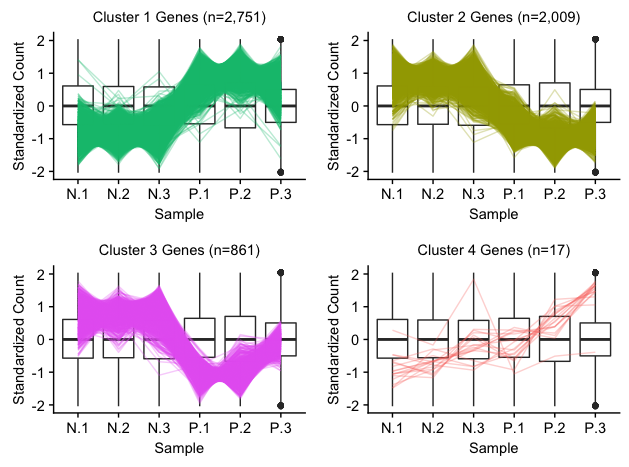
\includegraphics[width=\columnwidth]{MakeFigures/sbIRClustersSig.jpg}}
\end{framed}
\caption{Using parallel coordinate plots to visualize significant genes after hierarchical clustering. We can quickly confirm that Clusters 1 and 2 show the typical pattern for significant genes. Cluster 4 does not distinctively show the usual profile for significant genes. Cluster 3 looks similar to Cluster 2, except for unexpectedly large P.3 values.
\label{sbIRClustersSig}}
\end{figure}

\section{Scatterplot matrices}

\subsection{Overview of scatterplot matrices}

A scatterplot matrix is another effective multivariate visualization tool that plots the mapped read count distributions across all genes and samples. Specifically, it represents each row (gene) as a point in each scatterplot. With this method, users can quickly discover unexpected patterns, recognize geometric shapes, and assess the structure and association between multiple variables in a manner that is different from most common practices. 

Clean data would be expected to have larger variability between treatment groups than between replicates. As Figure~\ref{sbIRClustersSig} shows, researchers can quickly confirm this with a scatterplot matrix. Within each scatterplot, most genes should fall along the \textit{x=y} line (in red) as we expect only a small proportion of them to show differential expression between samples. However, a fraction of the genes should have lower variability between replicates than between treatments, and so we should expect the spread of the scatterplot points to fall more closely along the \textit{x=y} relationship between replicates than between treatments. Indeed, in Figure~\ref{sbIRClustersSig}, we created a scatterplot matrix for a public RNA-seq dataset that contains three replicates for two developmental stages of soybean cotyledon (S1 and S2) \citep{Brown}. We can immediately verify that the nine scatterplots between treatment pairs (in the bottom-left corner of the matrix) have more spread around the \textit{x=y} line than the six scatterplots between replicate pairs.

\begin{figure}[!tpb]
\begin{framed}
\centerline{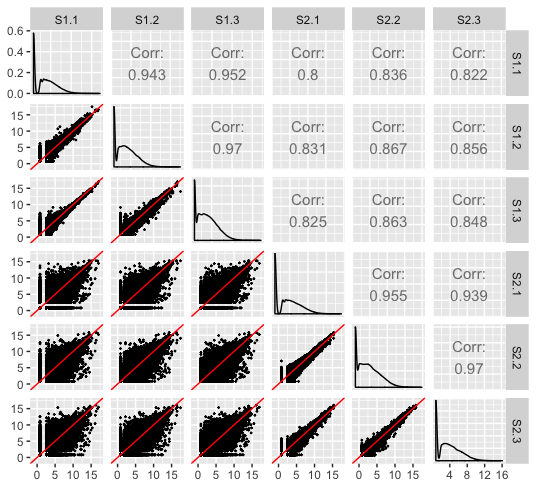
\includegraphics[width=\columnwidth]{MakeFigures/sbCNSM.jpg}}
\end{framed}
\caption{Example of the expected structure of an RNA-seq dataset, using soybean cotyledon data from \cite{Brown}. Within a given scatterplot, most genes (points) should fall along the \textit{x=y} line. We should see genes deviate more strongly from the \textit{x=y} line in treatment scatterplots than in replicate scatterplots. 
\label{sbCNSM}}
\end{figure}

After confirming this expected trend, users can use the scatterplot matrix to focus on subsets of genes: Outlier genes that deviate from the \textit{x=y} line in replicate scatterplots might be problematic, whereas outlier genes that deviate from the \textit{x=y} line in treatment scatterplots might be DEGs. In order to achieve this functionality, the plots must be rendered interactive.

Notice that each gene in our data is plotted once in each of the 15 scatterplots. With 73,320 genes in our data, more than one million points must be plotted. Rendering all points interactive would slow down the interactive capabilities of the plot. To solve this, we can tailor the geometric object of the scatterplots to be hexagon bins rather than points. This dramatically reduces the number of geometric objects to be plotted, and increases the interactivity speed.

The reader can visit https://rnaseqvisualization.shinyapps.io/scatmat to access the interactive version of Figure~\ref{sbCNSM}. Readers can read the ``About" Tab to fully understand how to use the application. Essentially, the user can hover over a hexagon bin to see how many genes it contains. When the user clicks on a hexagon bin, the names of the genes are listed and superimposed as orange points across all scatterplots. The genes are also linked to a second plot that superimposes them as parallel coordinate lines on a side-by-side boxplot of all gene counts. This interactivity and linking allows users to quickly examine genes of interest from multiple perspectives superimposed onto the summary of all genes in the dataset. 

\subsection{Assessing normalization with scatterplot matrices}

There is still substantial discussion about the normalization of RNA-seq data, and the scatterplot matrix can be used to understand and assess various algorithms. To exemplify this point, we will use a publicly-available RNA-seq dataset on Saccharomyces cerevisiae (yeast) grown in YP-Glucose (YPD) \citep{Risso}. The data contained four cultures from independent libraries that were sequenced using two library preparation protocols and either one or two lanes in a total of three flow-cells. This experimental design allowed researchers to examine various levels and combinations of technical effects (library preparation and protocol and flow cell) and biological effects (culture).

The four cultures (Y1, Y2, Y4, and Y7) were treated as biological replicates for which differential expression was not expected. Hence, the authors could establish a false positive rate in relation to the number of DEGs called between these groups. They then demonstrated that within-lane regression alone was insufficient in effectively removing biases. Instead, aggressive corrections for both within-lane (GC-content and gene length) and between-lane (count distribution and sequencing depth) biases were needed to effectively reduce the false-positive rate of differential expression calls.

Figure~\ref{yeastWithinBetween}A shows the scatterplot matrix of the read counts from the Y1 and Y4 treatments after within-lane normalization. As we stated earlier, we expect most genes to show similar expression between samples, except for the handful that are differentially expressed. However, it is immediately clear that the data still was not sufficiently normalized as the distribution of genes is not centered around the \textit{x=y} lines. In contrast, Figure~\ref{yeastWithinBetween}B shows the scatterplot matrix of the read counts from the Y1 and Y4 treatments after \textit{both} within-lane and between-lane normalization, as was recommended by the authors due to its reduced false-positive rate. Indeed, the scatterplot matrix now follows the expected structure with most genes falling along the \textit{x=y} line with thicker deviations from it between treatment groups than between replicate groups.

Additionally, we can also confirm from Figure~\ref{yeastWithinBetween}B that the read counts fall closer to the \textit{x=y} line between the Y4 replicates (bottom-right scatterplot) than between the Y1 replicates (top-left scatterplot). This is expected because the Y1 replicates had additional technical variability as they used two different flow cells, whereas the Y4 replicates were from the same flow cell. As such, the scatterplot matrix can also be used to quickly inspect patterns of biological and technical variability in the dataset.

\subsection{Checking for common errors with scatterplot matrices}

Irreproducibility is prevalent in high-throughput biological studies. A study in Nature Genetics surveyed eighteen published microarray expression analyses and reported that only two were exactly reproducible \citep{Ioannidis}. The extent of the problem has spawned a field called ``forensic bioinformatics" whereby researchers attempt to reverse-engineer reported results back into the raw datasets simply to derive the methodologies used in published studies \citep{Baggerly}.

\begin{figure}[!tpb]
\begin{framed}
\centerline{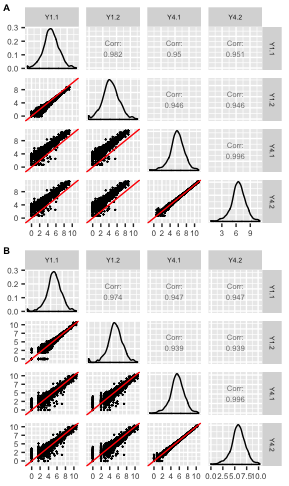
\includegraphics[width=0.8\columnwidth]{MakeFigures/yeastWithinBetween.jpg}}
\end{framed}
\caption{Illustrating normalization checks with data from  \cite{Risso}. The collective deviation of genes from the \textit{x=y} line instantly reveals that the RNA-seq dataset was not thoroughly normalized using within-lane normalization (subplot A). However, within-lane normalization followed by between-lane normalization sufficiently normalized the data (subplot B). The authors who developed these normalization methods showed that the later approach generated a lower false-positive DEG call rate in this dataset.
\label{yeastWithinBetween}}
\end{figure}

Even though irreproducibility is merely cumbersome when it masks methods, it is unquestionably hazardous when it masks errors. With regards to personalized medicine, for example, obscured errors may cause well-intentioned researchers to present evidence for drugs that are ineffective or even harmful to patients \citep{Baggerly}. Forensic bioinformaticians who have actively investigated common errors in high-throughput biological studies have concluded that the largeness of the data itself may hinder our ability to detect errors \citep{Baggerly}. They also discovered that the most common errors are simple errors, such as mixing up sample labels \citep{Baggerly}. Collectively, these findings suggest that simple errors can be difficult to detect using common practices in high-throughput studies.

Fortunately, scatterplot matrices are a simple tool to check for common errors like sample mislabeling. Figure~\ref{sbCNSwitchedSM} shows the resulting scatterplot matrix after we deliberately swapped the labels of the third replicate of the first treatment group (S1.3) with the first replicate of the second treatment group (S2.1) in the previously-mentioned cotyledon dataset. We can immediately see that, as expected, there are nine scatterplots with thicker distributions around the \textit{x=y} line and six scatterplots with thinner distributions around the \textit{x=y} line. However, we notice that a subset of these thick and thin scatterplots appear outside of their expected locations given the expected variability between treatments versus replicates. Rearranging the columns of the two samples that appear suspicious in Figure~\ref{sbCNSwitchedSM} would indeed lead us back to the clean-looking scatterplot matrix we saw in Figure~\ref{sbIRClustersSig}. We cannot detect this mislabeling problem as convincingly with traditional plots, as can be verified with this dataset by comparing the boxplots and MDS plots before sample switching (left side of Supplementary Figure~\ref{mdsSwitch}) and after sample switching (right side of Supplementary Figure~\ref{mdsSwitch}). 


\subsection{Finding unexpected patterns in scatterplot matrices}

Most popular RNA-seq plotting tools display summaries about the read counts, such as fold change summaries, principal component summaries, five number summaries, and dispersion summaries. In contrast to this trend, scatterplot matrices display the non-summarized read counts for all genes. This trait allows for geometric shapes and patterns relevant to the read count distribution to be readily visible in the scatterplot matrix.

An example of how geometric shapes in the scatterplot matrix can provide applicable information to researchers is shown in Figure~\ref{structure}, which uses the iron-metabolism soybean dataset \citep{Lauter16}. After normalizing the data, we see the expected pattern of a scatterplot matrix, with more variation around the \textit{x=y} line between treatments than between replicates (Figure~\ref{structure}). 

%%%%%%%%%%%%%% Ask Michelle for thoughts below %%%%%%%%%%%%%%%%%%%
However, one streak structure in the bottom right scatterplot stands out. A small subset of transcripts between replicates of the iron-sufficient group sharply deviates from the \textit{x=y} line. By interacting with the plot, we determined the identification of the five transcripts that deviated the most from the expected pattern, and searched for their putative functions. We discovered that these transcripts are reportedly involved in biotic and abiotic stress responses as well as the production of superoxides to combat microbial infections. This is the same group of genes discussed in Figure~\ref{sbIRClustersSig}. It should be noted that these five transcripts did not reach significance unless the third replicate of the P group was removed. In any case, we would not have observed this interesting structure from any models.

\begin{figure}[!tpb]
\begin{framed}
\centerline{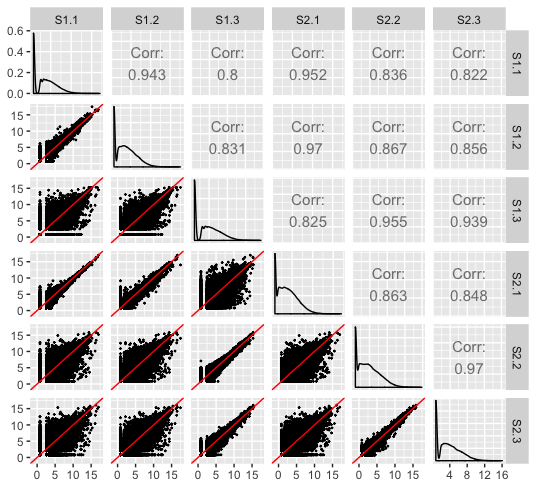
\includegraphics[width=\columnwidth]{MakeFigures/sbCNSwitchedSM.jpg}}
\end{framed}
\caption{As expected, this scatterplot matrix contains nine scatterplots with thicker distributions (should be treatment pairs) and six scatterplots with thinner distributions (should be replicate pairs). However, two samples appear to cause a subset of scatterplots to unexpectedly show thicker distributions between replicate pairs and thinner distributions between treatment pairs. If we switch the labels of these two suspicious samples (S1.3 and S2.1), the scatterplot matrix then displays the anticipated structure we saw in Figure~\ref{sbCNSM}. At this point, we have evidence that these two samples may have been mislabeled, and we may wish to confirm this suspicion and correct it before continuing with the analysis.
\label{sbCNSwitchedSM}}
\end{figure}

\begin{figure}[!tpb]
\begin{framed}
\centerline{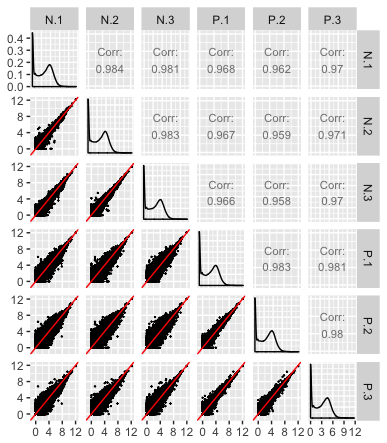
\includegraphics[width=\columnwidth]{MakeFigures/sbIRStreak.jpg}}
\end{framed}
\caption{Scatterplot matrix of RNA-seq read counts from soybean leaves after exposure to iron-sufficient (treatment group P) and iron-deficient (treatment group N) soil conditions~\citep{Lauter16}. We observe the expected structure of treatment pairs showing larger variability around the \textit{x=y} line than replicate pairs. However, we notice a pronounced streak structure in the bottom-right scatterplot that compares two replicate samples from the iron-sufficient group. The genes in the streak structure have large read counts that deviate in a parallel fashion from the \textit{x=y} line. Through contacting the authors of this dataset, we discovered that a leaf on one of these samples was inadvertently torn and then documented as such during the experiment. Hence, the genes within this streak structure might represent those that responded to this leaf-tearing event, an observation discovered through the scatterplot matrix that could solidify into a post-hoc hypothesis.
\label{structure}}
\end{figure}

\subsection{Assessing differential expression calls in scatterplot matrices}

The scatterplot matrix can also be used to quickly examine the DEGs returned from a given model. Figure~\ref{sbIRDEG} shows the DEGs from the soybean cotyledon dataset superimposed as orange points onto the scatterplot matrix. We expect for DEGs to fall along the \textit{x=y} line for scatterplots between replicates and deviate from the \textit{x=y} line for scatterplots between treatment groups, as is confirmed in Figure~\ref{sbIRDEG}. As a side note, we can also link these DEGs as parallel coordinate lines on a side-by-side boxplot like in Figure~\ref{sbIRDEG} to confirm the expected pattern of differential expression from a second viewpoint. If we do not observe what should be expected of DEGs, then the DEG calls from the model may need to be scrutinized further.

As an additional example, we overlaid the significant genes from the four clusters of the iron-metabolism soybean dataset (originally shown in Figure~\ref{sbIRClustersSig}) onto the scatterplot matrix. The results are shown and briefly discussed in Supplementary Figures~\ref{sbIRClusterSigSM1}-\ref{sbIRClusterSigSM1}. 

\section{Litre plots}

We demonstrated how to view differentially expressed genes onto the Cartesian coordinates of the scatterplot matrix in Figure~\ref{sbIRDEG}. Unfortunately, this figure becomes limited when we investigate treatment groups that contain a large number of replicates because we then have too many small scatterplots for it to remain an effective visualization tool. Moreover, researchers could benefit from additional plotting tools that allow them to quickly verify individual differentially expressed genes returned from a model. As a result, we developed a plot that allows users to visualize \textit{one} differentially expressed gene of interest onto the Cartesian coordinates of \textit{one} scatterplot matrix.

The ``replicate line plot" was developed by a group of researchers who demonstrated it could detect model scaling problems in microarray data \citep{Cook}. Unfortunately, this plot is only applicable on datasets where treatment groups contain exactly two replicates. The plot we now introduce is an extension of the ``replicate line plot" that can be applied to datasets with two or more replicates. We call this new plot a repLIcate TREatment (``litre") plot.

In the litre plot, each gene is plotted once for each possible combination of replicates between treatment groups. For example, there are nine ways to pair a replicate from one treatment group with a replicate from the other treatment group in the soybean iron-metabolism dataset (N.1 and P.1, N.1 and P.2, N.1 and P.3, N.2 and P.1, N.2. and P.2, N.2 and P.3, N.3 and P.1, N.3 and P.2, and N.3 and P.3). Hence, a given gene from this dataset is plotted as nine points in the litre plot. With 56,044 genes in this dataset, we would need to plot 504,396 points. This would reduce the speed of interactive functionality as well as cause overplotting problems. As a result, we again use hexagon bins to summarize this massive information (Figure~\ref{repDot} shows four example litre plots).

Once the background of hexagons has been drawn to give us a sense of the distribution of all treatment pair combinations for all genes, the user can superimpose the nine points of one gene of interest. We can examine and compare litre plots using the clusters we created in Figure~\ref{sbIRClustersSig}. Subplots A and B of Figure~\ref{repDot} each show a significant gene from Cluster 2 plotted as nine mustard points, subplots C and D each show a significant gene from Cluster 3 plotted as nine pink points, and subplots E and F each show a significant genes from Cluster 4 plotted as nine coral points. Note that, in the examples in Figure~\ref{repDot}, the read counts of treatment pair combinations sometimes overlap, resulting in the appearance of less than nine points being overlaid. Example litre plots from Cluster 1 are shown in Supplementary Figure~\ref{litreCluster1}.

\begin{figure}[!tpb]
\begin{framed}
\centerline{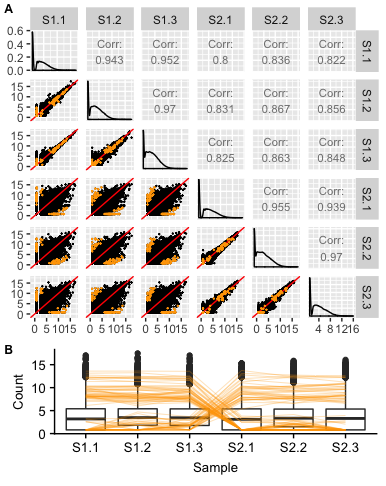
\includegraphics[width=\columnwidth]{MakeFigures/sbIRDEG.jpg}}
\end{framed}
\caption{Example of the expected structure of DEG calls (in orange) from an RNA-seq dataset. In the scatterplot matrix (subplot A), DEGs should fall along the \textit{x=y} line for replicates and deviate from it for treatments. In the parallel coordinate plot (subplot B), DEGs should show levelness between replicates and crosses between treatments. These two plotting types can be linked to quickly provide users multiple perspectives of their DEG calls.
\label{sbIRDEG}}
\end{figure}

\begin{figure}[!tpb]
\begin{framed}
\centerline{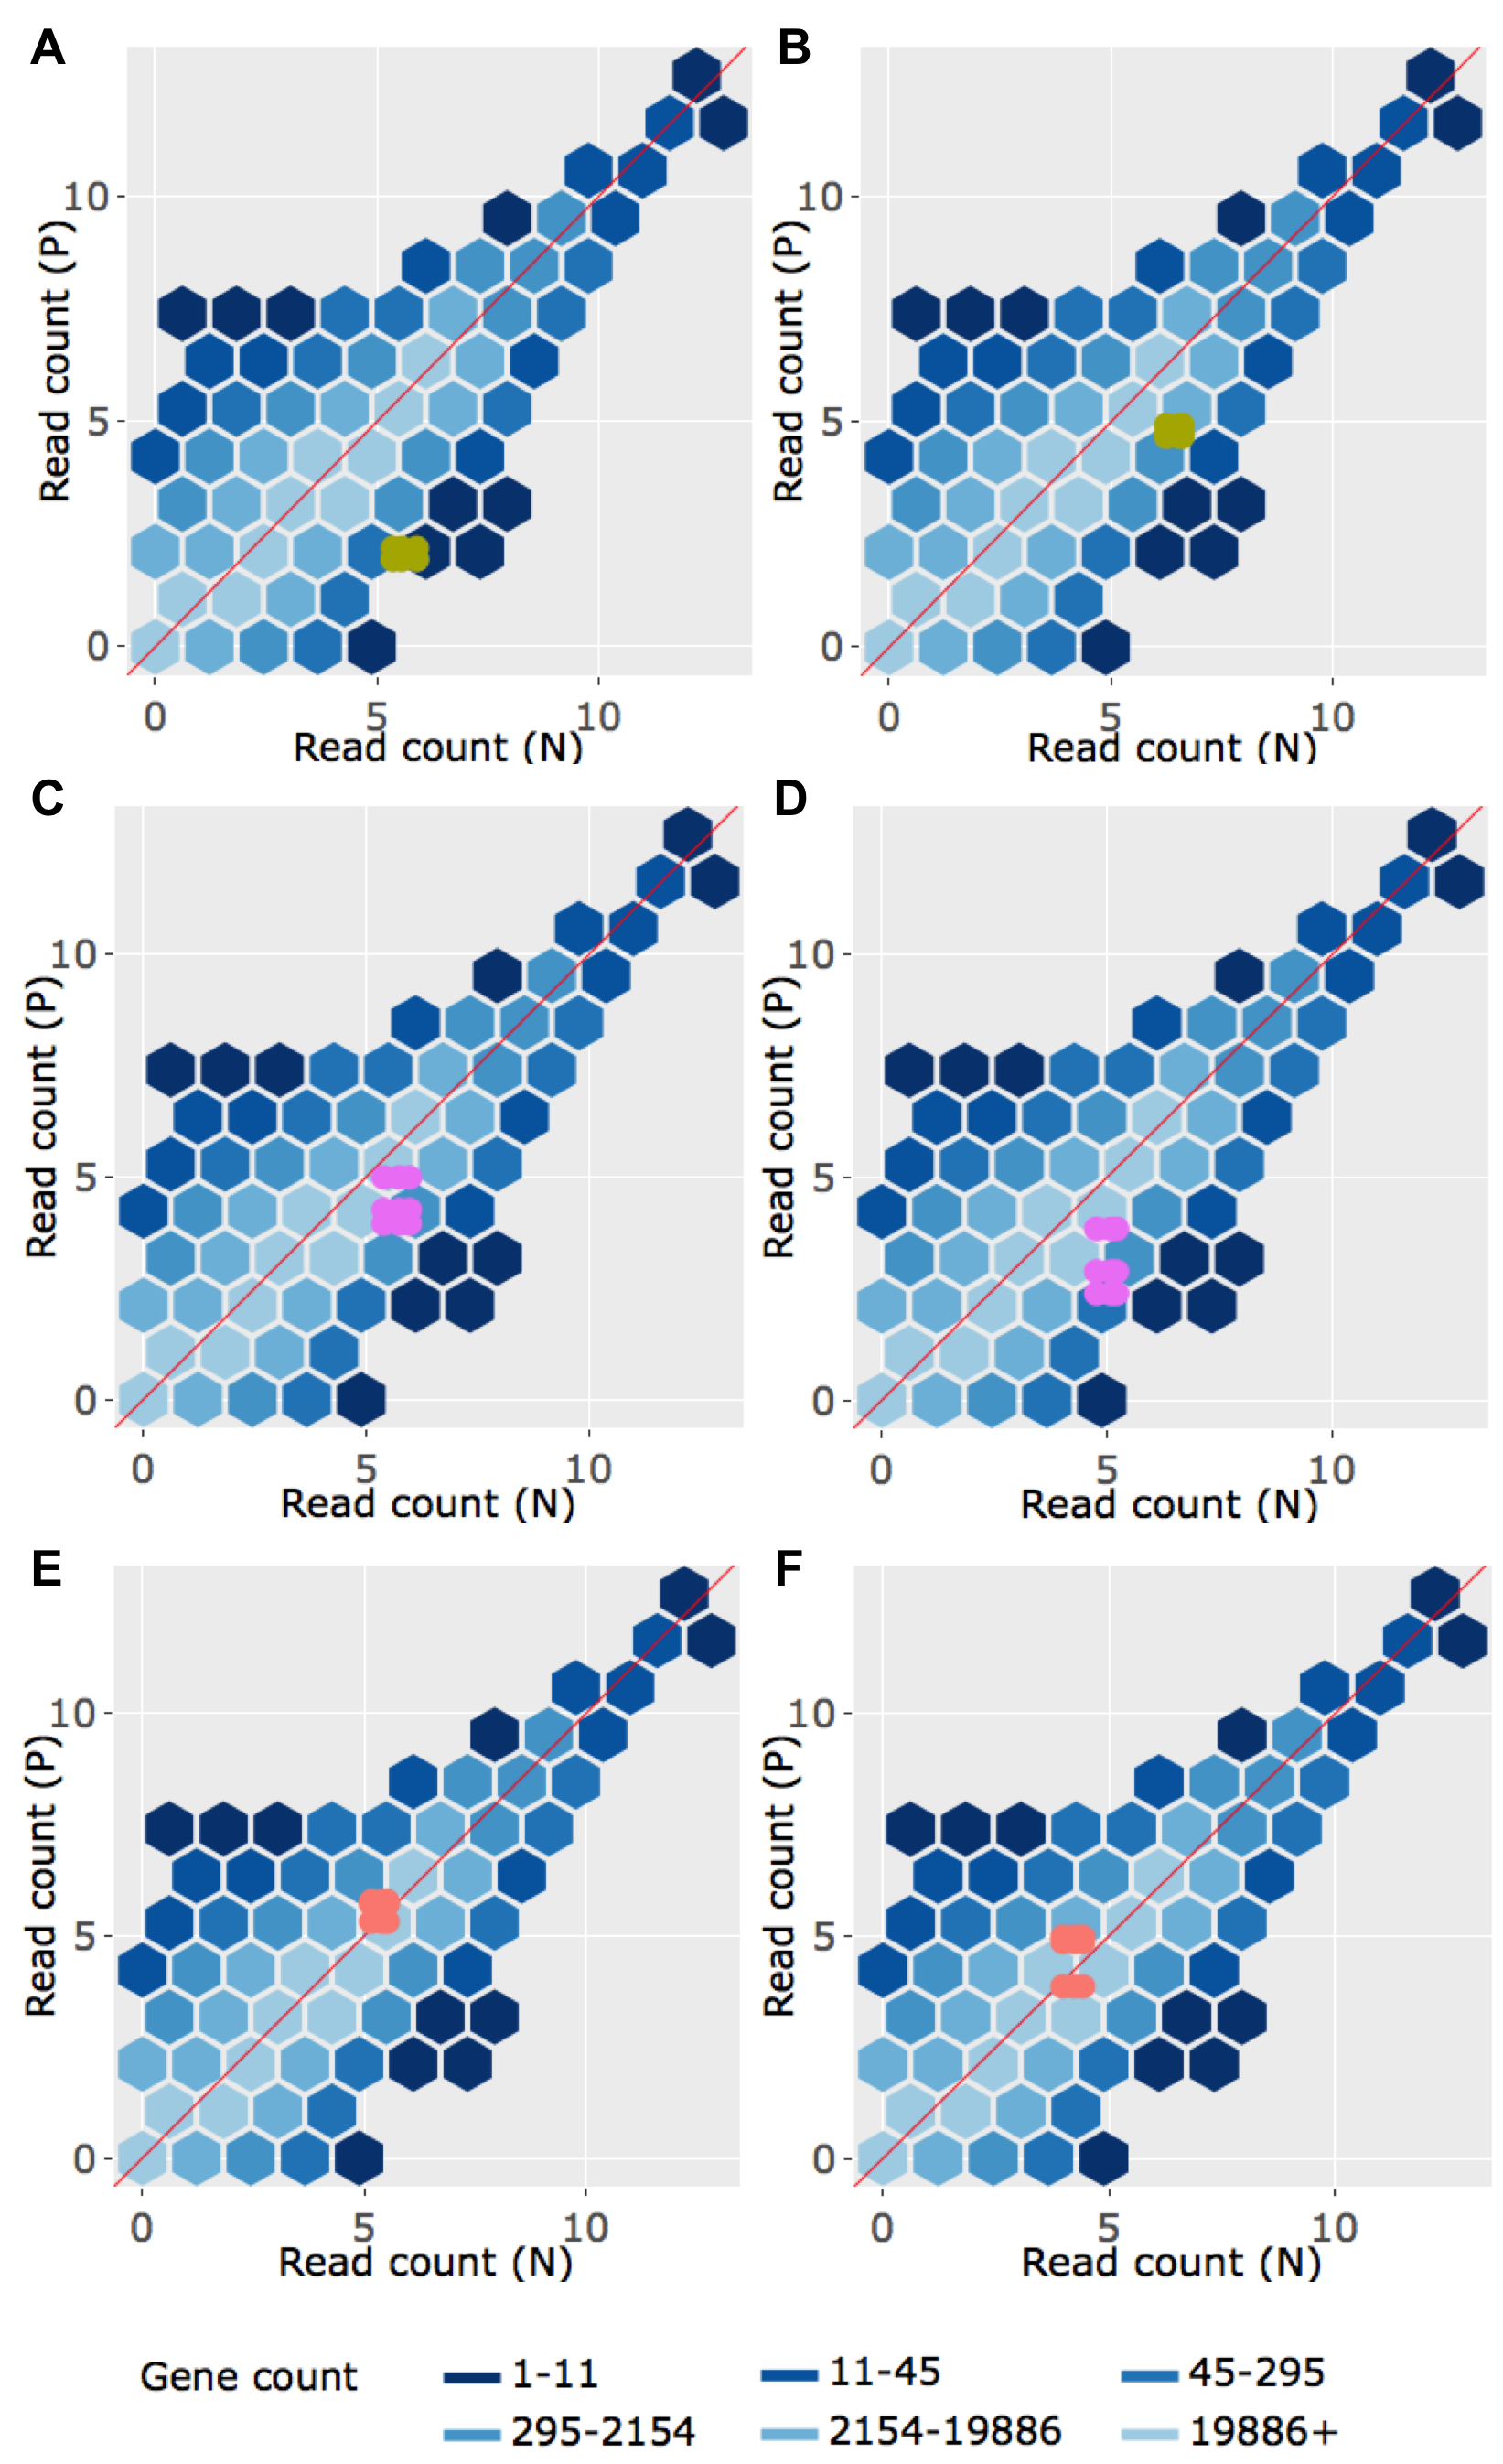
\includegraphics[width=0.85\columnwidth]{MakeFigures/litre6LB.png}}
\end{framed}
\caption{Litre plots for representative genes from clusters created in Figure~\ref{sbIRClustersSig}. Subplots A and B each show a gene from Cluster 2 overlaid as nine mustard points. Subplots C and D each show a gene from Cluster 3 overlaid as nine pink points. Subplots E and F each show a gene from Cluster 4 overlaid as nine coral points. Litre plots allow us to quickly flip through genes and search for (possibly odd) patterns that may not be detected numerically.
\label{repDot}}
\end{figure}

For the case of Figures~\ref{repDot} A and B, the nine overlaid points are superimposed in a manner we would expect from a differently expressed gene: They are located far from the \textit{x=y} line (difference between treatments) and are close to each other (similarity between replicates). In fact, the replicates in subplot B are so precise that the overlaid points almost entirely overlap each other. In contrast, Figures~\ref{repDot} C and D do not seem to show as much replicate consistency. Now, there seems to be a pattern in which one replicate from the P group is larger than (and visually distanced from) the other two replicates. In other words, litre plots are able to capture the pattern differences in the significant genes from Cluster 2 and 3 that we saw back in Figure~\ref{sbIRClustersSig}.

Moreover, in the case of Figures~\ref{repDot} E and F, the nine overlaid points are not clearly superimposed in the distinct pattern we expect of significant genes. While subplot E shows a gene that has consistent replications, the difference between the treatment groups is so small that the overlaid points cluster around the \textit{x=y} line. Additionally, the gene displayed in subplot F shows inconsistent replications and consistent treatment groups, as the spread-out overlaid points center on the \textit{x=y} line. Despite these genes being deemed significant by the model, the litre plots call into question whether the genes from this cluster show an expected profile of differential expression. This is similar to the messy-looking parallel coordinate plots we saw from these genes in Cluster 4 back in Figure~\ref{sbIRClustersSig} and the messy-looking superimposition we saw from these genes in Cluster 4 onto the scatterplot matrix in Supplementary Figure~\ref{sbCNSwitchedSM}. As a result, litre plots can detect odd and questionable patterns in individual ``significant genes" that cannot be detected numerically through models. If this happens, the user may wish to further investigate these DEG calls.

The interactive litre plot for the Cluster 2 significant genes (Figure~\ref{repDot} A and B) is available at https://rnaseqvisualization.shinyapps.io/litreCluster2, the interactive litre plot for the Cluster 3 significant genes (Figure~\ref{repDot} C and D) is available at https://rnaseqvisualization.shinyapps.io/litreCluster3, and the interactive litre plot for the Cluster 4 significant genes (Figure~\ref{repDot} E and F) is available at https://rnaseqvisualization.shinyapps.io/litreCluster4. As can be verified in the interactive version of the litre plot, users are provided several input fields that tailor the plot functionality. For instance, the user may wish to quickly scroll through significant genes one by one in the order of lowest to highest FDR values. Please read the ``About" tab in the interactive links for more information.

\section{Closing case study}

We briefly discuss an additional example that merges many of the topics addressed in this paper. The publicly available data for this example contain technical replicates of liver and kidney RNA samples \citep{Marioni}. We first calculate DEG calls for this data using the popular normalization method of library size scaling, where the number of total reads in each sample are normalized to a common value across all samples. This process leads to 9,018 DEGs, with most of them ($\sim$78\%) showing higher expression in the kidney group.

Although we could finish our analysis at this point and draw conclusions based on this list of DEGs that came from the model, it would be wise to also view this dataset visually. Viewing this data as a scatterplot matrix confirms the expected pattern with treatment scatterplots showing larger variation than technical replicate scatterplots. However, it also uncovers a hidden pattern in the treatment plots: There is a pronounced streak of genes with higher expressions in the liver group (Figure~\ref{lkSM}). We should also view the DEGs from the model using parallel coordinate plots: Upon doing so, we notice that while the 1,968 liver-specific DEGs follow the expected pattern of significant calls, a substantial fraction of the 7,050 kidney-specific DEGs appear comparatively noisy (Figure~\ref{lkClusters}A).

\begin{figure}[!tpb]
\begin{framed}
\centerline{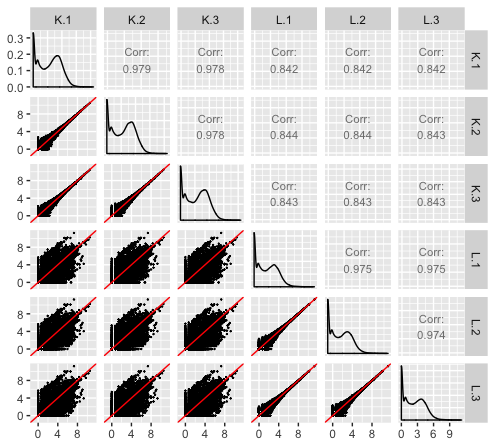
\includegraphics[width=1\columnwidth]{MakeFigures/lkSM.jpg}}
\end{framed}
\caption{Scatterplot matrix of liver and kidney technical replicates. The technical replicate scatterplots look precise as is expected, with little variability around the \textit{x=y} line. The treatment group scatterplots have much more variability around the \textit{x=y} line, as we would expect. However, each treatment group scatterplot contains a pronounced streak of highly-expressed liver-specific genes, which deviates from the expected distribution. Some researchers have suggested that differences in the distribution of reads between groups may require particularly stringent normalization.
\label{lkSM}}
\end{figure}

\begin{figure}[!tpb]
\begin{framed}
\centerline{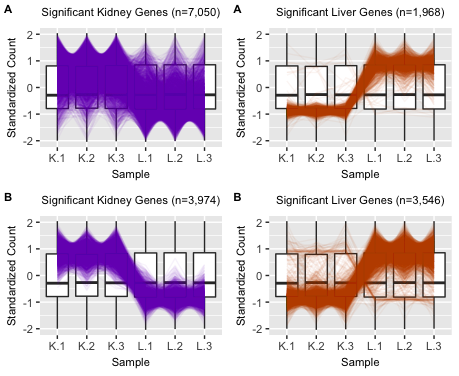
\includegraphics[width=1\columnwidth]{MakeFigures/lkClusters.jpg}}
\end{framed}
\caption{Subplot A shows parallel coordinate plots of the DEGs from liver and kidney technical replicates after standard library scale normalization. The division of DEGs between the two groups was rather disparate, with ~78\% of the DEGs being kidney-specific and only ~22\% of the DEGs being liver-specific. Also of note, while the parallel coordinate patterns of the liver-specific DEGs appear as expected, the patterns of the kidney-specific DEGs seem to show comparatively larger variability between the replicates. Subplot B shows parallel coordinate plots of the DEGs from liver and kidney technical replicates after TMM normalization. The division of DEGs between the two groups is more balanced than in Subplot A, with ~53\% of the DEGs being kidney-specific and ~47\% of the DEGs being liver-specific. Additionally, the parallel coordinate patterns of both the liver-specific and kidney-specific DEGs appear as expected and more consistent with each other.
\label{lkClusters}}
\end{figure} 

Taking both of these observations into account, we may need to reconsider our normalization technique. Some authors have argued that the popular library scaling method is not adequate in all cases, especially when the underlying distribution of reads between samples is inconsistent. In the current data, the observed streak of outlier genes that are highly expressed in the liver samples reduces the sequencing quota available to the remaning genes in these samples, which could create an articial inflation of the kidney-specific DEG calls. These authors have recommended TMM normalization for such cases (including for this particular dataset) as this technique generates sample scaling factors that consider sample distributions \citep{RobinsonOshlack}.

In light of all this, we return to square one and now apply TMM normalization to this data. This process leads to 7,520 DEGs that have a more level distribution between the kidney ($\sim$53\%) and liver ($\sim$47\%) groups. The scatterplot matrix did not appear differently from what we saw in Figure~\ref{lkSM} as both of these normalization methods are scaling procedures. However, we should visualize the new DEG calls. Plotting these DEGs as parallel coordinate lines paints a much cleaner picture from what we saw earlier, with most genes following the expected pattern of significance (Figure~\ref{lkClusters}B). Of the 7,050 kidney-specific DEGs we saw previously with library scaling normalization, only a cleaner-looking subset (n=3,974) of them remained as such using TMM normalization.

A deeper investigation of the effects of normalization on this data are shown in the supplementary material. These visualizations collectively suggest that this datasest indeed requires more than just library scaling for reliable analysis. This case study was meant to underscore the overarching theme of this paper that iteration between models and visualizations is crucial to achieve the most convincing results and conclusions in RNA-seq studies.

\section{Discussion}

In this paper, we strived to convince readers that effective visualization should be a crucial part of RNA-seq analysis. We used real data to demonstrate that scatterplot matrices, parallel coordinate plots, and litre plots can help users check for normalization problems, catch common errors in the analysis pipeline, and confirm that the variation between replicates and treatments is as expected. We also showed that these graphical tools allow researchers to quickly explore lists of DEGs that come out of models and ensure which ones make sense from an additional and arguably more intuitive vantage point. Moreover, we demonstrated that our simple plotting tools allow researchers to discover genes of interest through visual geometric patterns that would otherwise remain undiscovered with models.

In general, scientists might uncover surprising patterns lurking in their data with plots in ways that cannot be achieved with any formulas or models. Researchers from all statistical backgrounds can use graphical tools to better understand (if not demystify) how the application of various normalization techniques and/or models affect their results. All in all, scientists can gain more confidence in the data analysis pipelines they choose and in the results they draw at the mere cost of briefly creating and exploring graphical outputs during their analyses.

Modern data analysis is most reliable when models and visuals are used congruently. Unfortunately, the current culture around RNA-seq analysis de-emphasizes the importance of graphical tools, which, as we have shown, calls into question the soundness of results that come from RNA-seq studies. Solving this problem is simple and does not require scientists to drastically change their approach to RNA-seq analysis. Instead, scientists simply need to incorporate effective plotting tools during their usual analysis pipelines. We plan to serve a role in this solution by publishing a new \textsf{R} software package that includes the useful plotting techniques we introduced in this paper. To encourage scientists to use this resource, we aim to include a straight-forward vignette that demonstrates how to painlessly apply these graphical tools to RNA-seq data. It is our hope that such work will serve a small part in upgrading the RNA-seq analysis world into one that more wholistically extracts meaningful biological information using both models and visuals.

\section{Acknowledgments}

This project was an effort between Dianne Cook and myself, as well as the research of Michelle Graham and Adrianne Moran Lauter, from which the iron-metabolism soybean dataset was shared. The work of Graham and Moran Lauter was financed by the United States Department of Agriculture, Agricultural Research Service (USDA-ARS) CRIS Project 5030-21220-005-00D and the Iowa Soybean Association.


%%%%%%%%%%%@@@@%%%%%%%%%%%%%%%%%%%%%%%%%% CHAPTER %%%%%%%%%%%%%%%%%%%%%%%%%%%%%%%%%%%%%% 
%%%%%%%%%%%%%%%%%%%%%%%%%%%%%%%%%%%%%%%%%%%%%%%%%%%%%%%%%%%%%%%%%%%%%%%%%%%%%%%%%%%%%

\chapter{Software for visualization methods in RNA-sequencing data analysis}
\label{sec:chapter3}

\section{Introduction}

As was discussed in chapter~\ref{sec:chapter2}, high-throughput sequencing methods produce large amounts of sequence data that have become more attainable and affordable in recent years. While this technology grants scientists with access to more information about their transcriptomes of interest, it also presents a challenge for them in terms of requiring robust computational tools for the analysis of such unprecedented amounts of sequencing data. The typical analysis pipeline for RNA-sequencing data, for instance, identifies differentially expressed genes that are up and/or down regulated based on fold-changes when comparing between treatments of interest (such as healthy versus unhealthy tissues). Normalization is used within and/or between samples and statistical models are used to investigate the reliability of fold-change calculations for each gene by taking into account variation across genes and samples. Any genes that are identified as differentially expressed subsequently undergo functional enrichment to identify the involved gene ontological biological processeses, molecular functions, and cellular components. 

Chapter~\ref{sec:chapter2} showed several examples of why implementation of visualization methods that allow users to confirm the known and reveal the unknown in their RNA-sequencing data is an important procedure in the analysis, inference, and conclusions on their studies. In particular, visualizations that allow for users to assess the DEG calls from their RNA-sequencing studies is crucial to ensure that the subsequential functional enrichment analyses are provided reliable inputs. Most of the popular and free software packages that provide analysis pipelines for RNA-sequencing data do not use effective visualization tools, and if they do, they are often limited by their static nature (\citealt{deseq2}, \citealt{edger}, \citealt{limma}). In the past several years, new visualization approaches toward RNA-sequencing anaysis have incorporated interactive capabilities, and it is believed interaction trends will continue to enable enhanced visualization exploration of genomic datasets in the future (\citealt{vizReview}). Despite the growing appreciation of the inherent value of interactive graphics, the availability of easy-to-use and effective interactive exploratory visualization tools for RNA-sequencing data remains limited. To address this need, we are developing \pkg{bigPint}, an \pkg{R} software package that provides users with several new plotting techniques (introduced in chapter ~\ref{sec:chapter2}) in both static and interactive formats, as well as interactive versions of other popular plotting methods in RNA-sequencing analysis.

\section{Implementation}

Most interactive graphics in \pkg{bigPint} are constructed using \pkg{R} \citep{R} software, along with packages \pkg{ggplot2} (\citealt{ggplot2}), \pkg{Shiny} (\citealt{shiny}), \pkg{plotly} (\citealt{plotly}), and \pkg{htmlwidgets} (\citealt{htmlwidgets}). In many cases, \pkg{ggplot2} is used to create the main grammar of graphics of plots, while the ggplotly method from the \pkg{plotly} package is used to convert the ggplot object into a plotly object.

We also developed a collection of interactive graphics that share a rather unique feature: The background displays all genes in the dataset and the foreground displays a gene of interest (typically a DEG). Such functionality allows users to assess how the gene of interest in the foreground compares to the whole dataset, especially in terms of variability. As the number of genes in RNA-sequencing datasets is large and unchanging, the background plot should ideally remain static. However, the foreground plot of the gene of interest is small in size and can change depending on what specific gene the user wishes to examine. As a result, the foreground plot should ideally have interactive capabilities.
 
In order to acheive interactive functionality superimposed onto a static background, we could not simply rely on the onRender() method of the \pkg{plotly} package, because this would require the large background plot to be redrawn everytime a user interacts with any aspect of the graphic, causing unnecessary and substantial delays. Instead, we used the onRender() method from the \pkg{htmlwidgets} package. This method allows for the foreground data to be overlaid via plotly traces while the plotly background scatterplot matrix does not need to be redrawn. Specifically, it contains three input parameters, an HTML Widget object, a character vector containing JavaScript code, and a list of R objects that can be serialized to JSON format. In our case, we used a plotly object as the HTML Widget object, which allowed for a background that is static by default but can be changed if deliberately done so by the user. We used the JavaScript code parameter to allow for interactive manipulation of the overlaid gene of interest, and we used the R object list to transfer the count table and DEG list into the functionality.

In some our our graphics, users can link between interactive plots. This functoinality was achieved by sending custom messages between \pkg{Shiny} software and the JavaScript code from \pkg{htmlwidgets}.

\section{Supported data types}

Our software methods support the main types of input and output data structures from popular RNA-sequencing analysis software (\citealt{deseq2}, \citealt{edger}, \citealt{limma}). For many of our plotting methods, the input parameters include a count table of the entire dataset (can be raw, normalized, or standardized) and a list of a subset of this dataset (usually the DEGs) that came also come along with certain metrics of interest (such as fold-change and FDR). These input parameters are intended to allow our software tools to be easily incorporable into popular RNA-sequencing analysis software (\citealt{deseq2}, \citealt{edger}, \citealt{limma}), which often require the same count table as input and generate the subset of interest (usually the DEGs) along with metrics as output. 

\section{Examples Methods}

In chapter~\ref{sec:chapter2}, we provided users with access to an interactive scatterplot matrix from our software for them to explore (https://rnaseqvisualization.shinyapps.io/scatmat). We now also include a pre-made video to ensure users can understand some of the features available in our interactive graphics. The video in Figure~\ref{fig:scatMatPi} demonstrates a special variant of the interactive scatterplot matrix in which the user can select a prediction interval threshold to be applied to each scatterplot. In the video, the user can select individual genes of interest outside the prediction interval to highlight them across all scatterplots, while also superimposing them as parallel coordinate lines in a separate plot below. The user can also hover over genes of interest to elicit information about them. Although it is not shown in the video below, there are also several additional interactive features available through the Plotly Modebar, including zooming in an dout, reseting axes, autoscaling, and panning. The package also offers additional variations of the interactive scatterplot matrix, which are demonstrated in the supplemental information for this chapter (Section~\ref{sec:suppchapter3}). 

\begin{figure}[H]
    \begin{framed}
    \centering
    \includemedia[width=1.0\textwidth, addresource=scatMatPi.mov, deactivate=onclick, flashvars={source=scatMatPi.mov}]{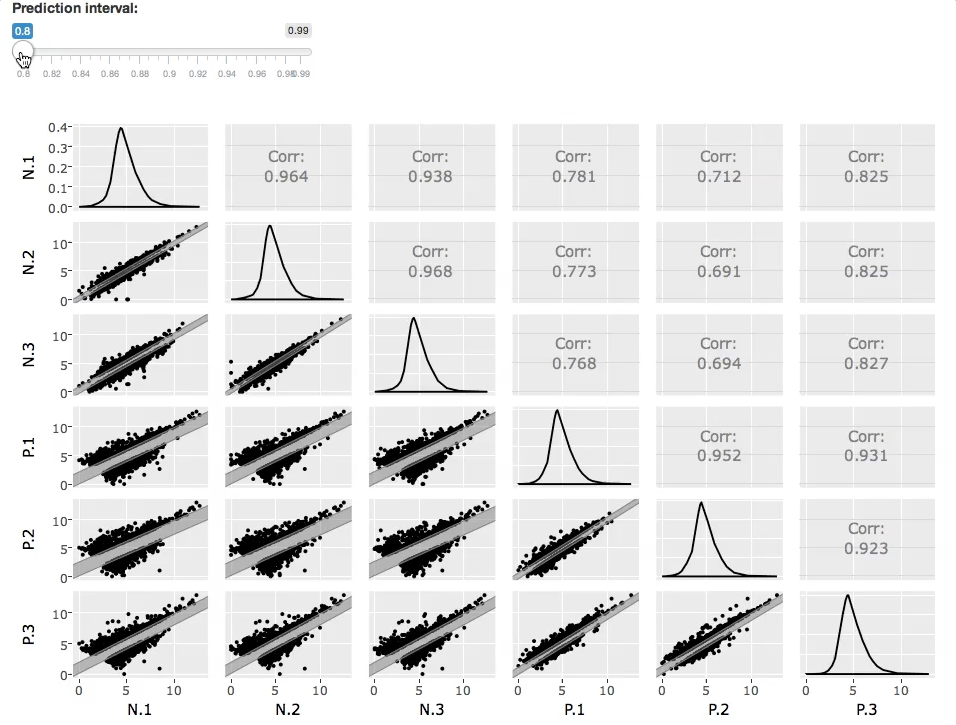
\includegraphics{./scatMatPi.jpg}}{VPlayer.swf}
    \end{framed}
    \caption{This video demonstrates an interactive scatterplot matrix that can be thresholded based on prediction interval. Upon clicking on this figure twice, a short video demonstrating the animation features for this function can be viewed. Please note that to properly view this video, the PDF version of this paper must be opened in Adobe Acrobat Reader DC (Version >=9), which can be downloaded free of charge.}
    \label{fig:scatMatPi}
\end{figure}

We demonstrate another example of a visualization method in RNA-sequencing analysis called the volcano plot (Video in figure~\ref{fig:volcano}). This plot is a type of scatterplot that draws significance versus fold-change on the axes. It usually offered in a static format. Here, we allow interactive features so the user can threshold based on either of the axes metrics, select genes of interest and simultaneously plot them in a linked parallel coordinate plot, and switch between treatment pairs within the dataset effortlessly.

\begin{figure}[H]
    \begin{framed}
    \centering
    \includemedia[width=1.0\textwidth, addresource=volcano.mov, deactivate=onclick, flashvars={source=volcano.mov}]{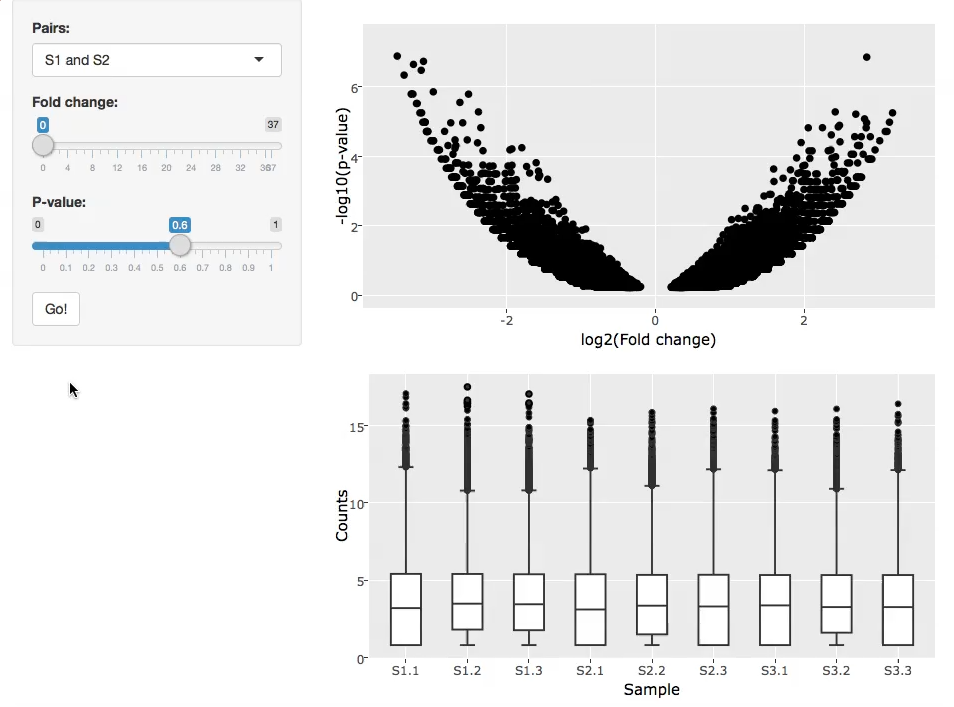
\includegraphics{./volcano.jpg}}{VPlayer.swf}
    \end{framed}
    \caption{This video demonstrates an interactive volcano plot. Upon clicking on this figure twice, a short video demonstrating the animation features for this function can be viewed. Please note that to properly view this video, the PDF version of this paper must be opened in Adobe Acrobat Reader DC (Version >=9), which can be downloaded free of charge.}
    \label{fig:volcano}
\end{figure}

\section{Discussion}

The plotting methods we offer in \pkg{bigPint} allow users to quickly and interactively examine genes of interest across the entire dataset. We integrate several technologies to achieve the useful and efficient functionality that allows for an interactive foreground and a static background. Some of the graphics we offer in this package are not used in popular RNA-sequencing packages, such as scatterplot matrics, parallel coordinate plots, and litre plots. See chapter~\ref{sec:chapter2} for a review of these visualization tools. We also offer interactive versions of graphics that are already popular in RNA-sequencing packages, such as the volcano plot.

We plan to publish our software freely on Bioconductor, which provides open source software for bioinformatics. Our software can be used on Windows, MacOS, and Linux operating systems and will integrate neatly into popular RNA-sequencing analysis tools. The current version of our reference manual is posted as supplementary information in Section~\ref{sec:suppchapter3}. Analysis of large genomics data is relying more on sophisticated and interactive visualization techniques (\citealt{vizReview}) and we believe we will contribute to that promising trend by publishing our software.

\section{Acknowledgments}

This project was an effort between Dianne Cook and myself, along with helpful support and feedback from Roxane Legaie.

%%%%%%%%%%%@@@@%%%%%%%%%%%%%%%%%%%%%%%%%% CHAPTER %%%%%%%%%%%%%%%%%%%%%%%%%%%%%%%%%%%%%% 
%%%%%%%%%%%%%%%%%%%%%%%%%%%%%%%%%%%%%%%%%%%%%%%%%%%%%%%%%%%%%%%%%%%%%%%%%%%%%%%%%%%%%

\chapter{Gene expression responses to diet quality and viral infection in \textit{Apis mellifera}}
\label{sec:chapter4}

\section{Introduction}

Commercially managed honey bees have undergone unusually large declines in the United States and parts of Europe over the past decade (\citealt{ccd1}, \citealt{ccd2}, \citealt{ccd3}), with annual mortality rates exceeding what beekeepers consider sustainable (\citealt{ccd5}, \citealt{ccd6}). More than 70 percent of major global food crops (including fruits, vegatables, and nuts) at least benefit from pollination, and yearly insect pollination services are valued wordwide at \$175 billion (\citealt{ccd7}). As honey bees are largely considered to be the leading pollinator of numerous crops, their marked loss has considerable implications regarding agricultural sustainability (\citealt{ccd4}).

Honey bee declines have been associated with several factors, including pesticide use, parasites, pathogens, habitat loss, and poor nutrition (\citealt{factors}, \citealt{factors2}). Researchers generally agree that these stressors do not act in isolation; instead, they appear to influence the large-scale loss of honey bees in interactive fashions as the environment changes (\citealt{interacting}). Nutrition and viral infection are two broad factors that pose heightened dangers to honey bee health in response to recent environmental changes.

Pollen is the main source of nutrition (including proteins, amino acids, lipids, sterols, starch, vitamins, and minerals) in honey bees (\citealt{source}, \citealt{source2}). At the individual level, pollen supplies most of the nutrients necessary for physiological development (\citealt{brodschneider}) and is believed to have considerable impact on longevity (\citealt{longevity}). At the colony level, pollen enables young workers to produce jelly, which then nourishes larvae, drones, older workers, and the queen (\citealt{jelly}, \citealt{jelly2}). Various environmental changes (including urbanization and monoculture crop production) have significantly altered the nutritional profile available to honey bees. In particular, honey bees are confronted with less diverse selections of pollen, which is of concern because mixed-pollen (polyfloral) diets are generally considered healthier than single-pollen (monofloral) diets (\citealt{diverse}, \citealt{diverse2}, \citealt{alaux}). Indeed, reported colony mortality rates are higher in developed land areas compared to undeveloped land areas (\citealt{undeveloped}), and beekeepers rank poor nutrition as one of the main reasons for colony losses (\citealt{bkLoss}). Understanding how undiversified diets affect honey bee health will be crucial to resolve problems that may arise as agriculture continues to intensify throughout the world (\citealt{ag}, \citealt{ag2}).

Viral infection was a comparatively minor problem in honey bees until the last century when Varroa destructor (an ectoparasitic mite) spread worldwide (\citealt{miteSpread}). This mite feeds on honey bee hemolymph (\citealt{hemolymph}), transmits cocktails of viruses, and supports replication of certain viruses (\citealt{miteVirus}, \citealt{miteVirus2}, \citealt{miteVirus3}). More than 20 honey bee viruses have been identified (\citealt{numVirus}). One of these viruses that has been linked to honey bee decline is Israeli Acute Paralysis Virus (IAPV). A positive-sense RNA virus of the Dicistroviridae family (\citealt{fam}), IAPV causes infected honey bees to display shivering wings, decreased locomotion, muscle spams, and paralysis, and 80\% of caged infected adult honey bees die prematurely (\citealt{symptoms}). IAPV has demonstrated higher infectious capacities than other honey bee viruses in certain conditions (\citealt{carrillo}) and is more prevalent in colonies that do not survive the winter (\citealt{winter}). Its role in the rising phenomenon of ``Colony Collapse Disorder'' (in which the majority of worker bees disappear from a hive) remains unclear: It has been implicated in some studies (\citealt{iapvCCD}, \citealt{iapvCCD2}) but not in other studies (\citealt{ccd1}, \citealt{iapvCCD3}, \citealt{fam}). Nonetheless, it is clear that IAPV reduces colony strength and survival.

Although there is growing interest in how viruses and diet quality affect the health and sustainability of honey bees, as well as a recognition that such factors might operate interactively, there are only a small number of experimental studies thus far directed toward elucidating the interactive effects of these two factors in honey bees (\citealt{intNV}, \citealt{intNV2}, \citealt{intNV3}). We recently used laboratory cages and nucleus hive experiments to investigate the health effects of these two factors, and our results show the importance of the combined effects of both diet quality and virus infection. Specifically, high quality pollen is able to mitigate virus-induced mortality to the level of diverse, polyfloral pollen (\citealt{adamInt}). 

Following up on these phenotypic findings from our previous study, we now aim to understand the corresponding underlying mechanisms by which high quality diets protect bees from virus-induced mortality. For example, it is not known whether the protective effect of good diet is due to direct, specific effects on immune function (resistance), or if it is due to indirect effects of good nutrition on vigor (tolerance) (\citealt{resTol1}). Transcriptomics is one means to better understand the mechanistic underpinnings of dietary and viral effects on honey bee health. Transcriptomic analysis can help us identify 1) the genomic scale of transcriptomic response to diet and virus infection, 2) whether these factors interact in an additive or synergistic way on transcriptome function, and 3) the types of pathways affected by diet quality and viral infection. This information, heretofore lacking in the literature, can help us better understand how good nutrition may be able to serve as a "buffer" against other stressors (\citealt{AdamTothReview}). As it stands, there are only a small number of published experiments examining gene expression patterns related to diet effects (\citealt{alaux2}) and IAPV infection effects (\citealt{galbraith}) in honey bees. As far as we know, there are few to no studies investigating honey bee gene expression patterns specifically related to monofloral diets, and few to no studies investigating honey bee gene expression patterns related to the combined effects of diet in any broad sense and viral innoculation in any broad sense. 

In this study, we examine how monofloral diets and viral innoculation influence gene expression patterns in honey bees by focusing on four treatment groups (low quality diet without IAPV exposure, high quality diet without IAPV exposure, low quality diet with IAPV exposure, and high quality diet with IAPV exposure). We conduct RNA-sequencing analysis on a randomly selected subset of the honey bees we used in our previous study (as is further described in our methods section). We then examine pairwise combinations of treatment groups, the main effect of monofloral diet, the main effect of IAPV exposure, and the combined effect of the two factors on gene expression patterns.

We also compare the main effect of IAPV exposure in our dataset to that obtained in a previous study conducted by Galbraith and colleagues (\citealt{galbraith}). As RNA-sequencing data can be highly noisy, this comparison allowed us to characterize how repeatable and robust our RNA-seq results were in comparison to previous studies. Importantly, we use an in-depth data visualization approach to explore and corroborate our data, and suggest such an approach can be useful for cross-study comparisons and validation of noisy RNA-sequencing data in the future.

\section{Methods}

Details of the procedures we used to prepare virus inoculum, infect and feed caged honey bees, and quantify IAPV can be reviewed in our previous work (\citealt{adamInt}). The statistical analysis we used to study the main and interaction effects of the two factors on mortality and IAPV titers is also described in our earlier report (\citealt{adamInt}).

\subsection{Design of two-factor experiment}

There are several reasons why, in the current study, we focused only on diet quality (monofloral diets) as opposed to diet diversity (monofloral diets versus polyfloral diets). First, when assessing diet diversity, a sugar diet is often used as a control. However, such an experimental design does not reflect real-world conditions for honey bees as they rarely face a total lack of pollen (\citealt{DiPasquale}). Second, in studies that compared honey bee health using monofloral and polyfloral diets at the same time, if the polyfloral diet and one of the high-quality monofloral diets both exhibited similarly beneficial effects, then it was difficult for the authors to assess if the polyfloral diet was better than most of the monofloral diets because of its diversity or because it contained as a subset the high-quality monofloral diet (\citealt{DiPasquale}). Third, colonies used for pollination in agricultural areas (monoculture) face less diversified pollens (according to Brodschneider, 2010). Pollinating areas are currently undergoing landscape alteration and agriculture intensification, and bees are increasingly faced with less diversified diets (monoculture) (\citealt{landscape1}, \citealt{brodschneider}). As a result, there is a need to better understand how monofloral diets affect honey bee health as a step toward mitigating the negative impact of human activity on the honey bee population.

Consequently, for our nutrition factor, we examined two monofloral pollen diets, Rockrose (Cistus) and Castanea (Chestnut). Rockrose pollen is generally considered less nutritious than Chestnut pollen due to its lower levels of protein, amino acids, antioxidants, calcium, and iron (\citealt{DiPasquale}, \citealt{adamInt}). For our virus factor, one level contained bees that were infected with IAPV and another level contained bees that were not infected with IAPV. This experimental design resulted in four treatment groups (Rockrose pollen without IAPV exposure, Chestnut pollen without IAPV exposure, Rockrose pollen with IAPV exposure, and Chestnut pollen with IAPV exposure) that allowed us to assess main effects and interactive effects between diet quality and IAPV infection in honey bees.

\subsection{RNA extraction}

Fifteen cages per treatment were originally sampled. Six live honey bees from each cage were randomly selected 36 hours post inoculation and placed into tubes (\citealt{carrillo}). Tubes were kept on dry ice and then transferred into a -80C freezer until processing. Eight cages were randomly selected from the original 15 cages, and 2 honey bees per cage were randomly selected from the original six live honey bees per cage. Whole body RNA from each pool of two honey bees were extracted using Qiagen RNeasy MiniKit followed by Qiagen DNase treatment. Samples were suspended in water to 200-400 ng/$\mu$l. All samples were then tested on a Bioanalyzer at the DNA core facility to ensure quality (RIN>8).

\subsection{Gene expression}

Samples were sequenced starting on January 14, 2016 at the Iowa State University DNA Facility (Platform: Illumina HiSeq Sequencing; Category: Single End 100 cycle sequencing). A standard Illumina mRNA library was prepared by the DNA facility. Reads were aligned to the BeeBase Version 3.2 genome (\citealt{hbGenome}) from the Hymenoptera Genome Database (\citealt{hymenopteraDB}) using the programs GMAP and GSNAP (\citealt{gsnap}). There were four lanes of sequencing with 24 samples per lane. Each sample was run twice. Approximately 75-90\% of reads were mapped to the honey bee genome. Each lane produced around 13 million single-end 100 basepair reads. We tested all six pairwise combinations of treatments for DEGs (pairwise DEGs). We also tested the diet main effect (diet DEGs), virus main effect (virus DEGs), and interaction term for DEGs (interaction DEGs). We then also tested for virus main effect DEGs (virus DEGs) in public data derived from a previous study exploring the gene expression of IAPV virus infection in honey bees (\citealt{galbraith}). We tested each DEG analysis using recommended parameters with DESeq2 (\citealt{deseq2}), edgeR (\citealt{edger}), and LimmaVoom (\citealt{limma}). In all cases, we used a false discovery rate (FDR) threshold of 0.05 (\citealt{benjamini}). Fisher's exact test was used to determine significant overlaps between DEG sets (whether from the same dataset but across different analysis pipelines or from different datasets across the same analysis pipelines). The \pkg{eulerr} shiny application was used to construct Venn diagram overlap images (\citealt{euler}). In the main section of our paper and in subsequent analyses, we focus on the DEG results from DESeq2 (\citealt{deseq2}) as this pipeline was also used in the Galbraith study (\citealt{galbraith}).

\subsection{Comparison to previous studies on transcriptomic response to viral infection}

We also compare the main effect of IAPV exposure in our dataset to that obtained in a previous study conducted by Galbraith and colleagues (\citealt{galbraith}) who also addressed honey bee transcriptomic responses to virus infection.

While our study examines honey bees from polyandrous colonies, the Galbraith study examined honey bees from single-drone colonies. As a consequence, the honey bees in our study will be on average 25\% genetically identical, whereas honey bees from the Galbraith study will be on average 75\% genetically identical (\citealt{sisters}). We should therefore expect that the Galbraith study may generate data with lower signal:to:noise ratios than our data due to the lower genetic variation between its replicates. At the same time, our honey bees will be more likely to display the health benefits gained from increased genotypic variance within colonies, including decreased parasitic load (\citealt{multParasite}), increased tolerance to environmental changes (\citealt{divHyp2}), and increasead colony performance (\citealt{geneticDiverse}, \citealt{geneticDiverse2}). Given that honey bees are naturally very polyandrous (\citealt{patriline}), our honey bees may also reflect more realistic environmental and genetic simulations. Taken together, each study provides a different point of value: Our study likely presents less artificial data while the Galbraith data likely presents less messy data. We wish to explore how the gene expression effects of IAPV innoculation compare between these two studies that used such different experimental designs. To achieve this objective, we use visualization techniques to assess the signal:to:noise ratio between these two datasets, and differential gene expression (DEG) analyses to determine any significantly overlapping genes of interest between these two datasets. It is our hope that this aspect of our study may shine light on how experimental designs that control genetic variability to different extents might affect the resulting gene expression data in honey bees.

\subsection{Visualization}

We used various visualization tools as part of our analysis. First, we used popular tools (like the MDS plot) from the DESeq2 package. Second, we used multivariate visualization tools from our work-in-progress package called bigPint. Specifically, we used parallel coordinate plots, litre plots, and scatterplot matrices to assess the variability between the replicates and the treatments in our data and in the DEG outputs from applied models. We also used these plotting techniques to assess for normalization problems and other common problems in RNA-seq analysis pipelines. Third, we used visual inference techniques to assess the signal:to:noise ratio in the datasets and to assess the suitability of the DEG calls. 

\subsection{Gene Ontology}

DEGs were uploaded as a background list to DAVID Bioinformatics Resources 6.7 (\citealt{davidBio}, \citealt{davidBio2}). The overrepresented gene ontology (GO) terms of DEGs were determined using the BEEBASE\_ID identifier option (honey bee gene model) in the DAVID software. To fine-tune the GO term list, only terms correlating to Biological Processes were considered. The refined GO term list was then imported into REVIGO (\citealt{revigo}), which uses semantic similarity measures to cluster long lists of GO terms.

\subsection{Probing tolerance versus resistance}

To investigate whether the protective effect of good diet is due to direct, specific effects on immune function (resistance), or if it is due to indirect effects of good nutrition on energy availability and vigor (tolerance), we created contrasts of interest (Table \ref{tbl:contrasts}). In particular, we assigned ``resistance candidate genes" to be the ones that were upregulated in the Chestnut group within the virus infected bees but not upregulated in the Chestnut group within the non-infected bees. We also assigned "tolerance candidate genes" to be the ones that were upregulated in the Chestnut group for both the virus infected bees and non-infected bees. Our interpretation of these genes is that they represent genes that are constitutively activated in bees fed a high quality diet, regardless of whether they are experiencing infection or not. We then determined how many genes fell into these two categories and analyzed their GO terminologies.

\begin{table}[H]
\begin{tabular}{ | m{4.4cm} | m{0.9cm}| m{5.5cm} | m{2.6cm} | } 
\hline
Contrast & DEGs & Interpretation & Results \\ 
\hline
V (all) vs N (all) & 43 & Genes that change expression due to virus effect regardless of diet status in bees & Table \ref{tbl:virusGenes} \\ 
\hline
NC vs NR & 941 & Genes that change expression due to diet effect in uninfected bees & Supplementary tables \ref{tbl:NCNRNCPathways} and \ref{tbl:NCNRNRPathways} \\ 
\hline
VC vs VR & 376 & Genes that change expression due to diet effect in infected bees & Supplementary tables \ref{tbl:VCVRVCPathways} and \ref{tbl:VCVRVRPathways} \\ 
\hline
VC upregulated in VC vs VR overlapped with NC upregulated in NC vs NR & 122 & ``Tolerance'' genes that are turned on by good diet regardless of virus infection status in bees & Figure \ref{fig:revigo}A \\
\hline
VC upregulated in VC vs VR but NC is not upregulated in NC vs NR & 125 & ``Resistance'' genes that are turned on by good diet only in infected bees & Figure \ref{fig:revigo}B \\
\hline
\end{tabular}
\caption{Contrasts in our study for assessing GO and pathways analysis.}
  \label{tbl:contrasts}
\end{table}


\section{Results}

\subsection{Phenotypic results}

We reanalyzed our previously published dataset with a subset more relevant to our RNA-sequencing approaches in the current study that have a more focused question regarding diet quality. We briefly show it again here to inform the RNA-seq comparison because we reduced the number of treatments (from eight to four) from the original published data (\citealt{adamInt}) as a means to focus on diet quality effects.

Mortality rates of honey bees 72 hour post-inoculation significantly differed among the treatment groups (mixed model ANOVA across all treatment groups, df=3, 54; F=10.03; p<2.30e-05). The effect of virus treatment (mixed model ANOVA, df=1, 54; F=24.73; p<1.00e-05) and diet treatment (mixed model ANOVA, df=1, 54; F=5.32; p<2.49e-02) were significant, but the interaction between the two factors (mixed model ANOVA, df=1, 54; F=4.72e-02, p=8.29e-01) was not significant. We compared mortality levels based on pairwise comparisons: For a given diet, honey bees exposed to the virus showed significantly higher mortality rate than honey bees not exposed to the virus. Namely, bees fed Rockrose pollen had significantly elevated mortality with virus infection compared to uninfected controls (Tukey HSD, p<1.18e-03), and bees fed Chestnut pollen similarly had significantly elevated mortality with virus infection compared to controls (Tukey HSD, p<4.80e-03) (Figure \ref{fig:Mortality_Final}).

IAPV titers of honey bees 72 hour post-inoculation significantly differed among the treatment groups (mixed model ANOVA across all treatment groups, df=3, 33; F=6.10; p<1.96e-03). The effect of virus treatment (mixed model ANOVA, df=1, 33; F=15.04; p<4.75e-04) was significant, but the diet treatment (mixed model ANOVA, df=1, 33; F=2.55; p=1.20e-01) and the interaction between the two factors (mixed model ANOVA, df=1, 33; F=7.02e-01, p=4.08e-01) were not significant. We compared IAPV titer volumnes  based on pairwise comparisons: Bees fed Rockrose pollen had significantly elevated IAPV titer volumes with virus infection compared to uninfected controls (Tukey HSD, p<5.44e-03). However, bees fed Chestnut pollen did not have significantly elevated IAPV titer volumes with virus infection compared to uninfected controls (Tukey HSD, p=1.11e-01). Overall, we interpreted these findings to mean that high-quality Chestnut pollen could ``rescue'' high virus titers resulting from the inoculation treatment, whereas low-quality Rockrose pollen could not do so (Figure \ref{fig:IAPV_Final}).

\begin{figure}[H]
\centering
  \begin{framed}
  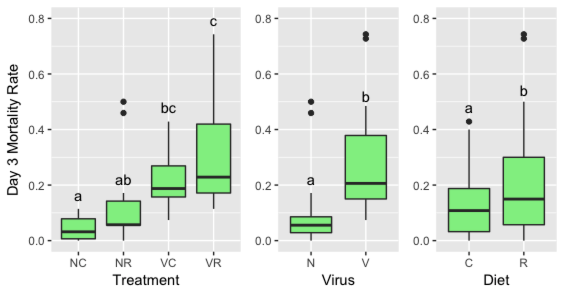
\includegraphics[width=\textwidth]{Images/Mortality_Final}
  \end{framed}
  \caption{Left to right: Mortality rates for the four treatment groups, two virus groups, and two diet groups. ``N'' represents non-inoculation, ``V'' represents viral inoculation, ``C'' represents Chestnut pollen, and ``R'' represents Rockrose pollen. The mortality rate data included 59 samples with 15 replicates per treatment group, except for the ``NC'' group having 14 replicates. ANOVA values and p-values for the statistical tests are listed in the text of the paper. The letters above the bars represent Tukey honest significant differences with a confidence level of 95\%.}
  \label{fig:Mortality_Final}
\end{figure}

\begin{figure}[H]
\centering
  \begin{framed}
  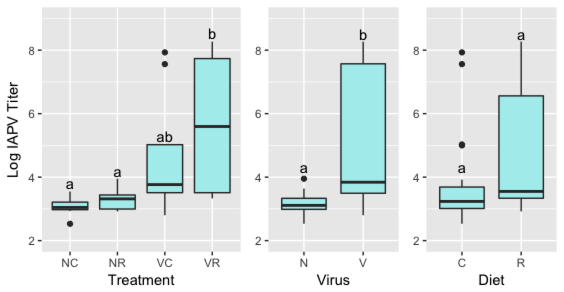
\includegraphics[width=\textwidth]{Images/IAPV_Final}
  \end{framed}
  \caption{Left to right: IAPV titer volumes for the four treatment groups, two virus groups, and two diet groups. ``N'' represents non-inoculations, ``V'' represents viral inoculation, ``C'' represents Chestnut pollen, and ``R'' represents Rockrose pollen. The IAPV titer data included 38 samples with 10 replicates per treatment group, except for the ``NR'' group having 8 replicates. ANOVA values and p-values for the statistical tests are listed in the text of the paper. The letters above the bars represent Tukey honest significant differences with a confidence level of 95\%.}
  \label{fig:IAPV_Final}
\end{figure}

\subsection{Main effect DEG results}

We observed a substantially larger number of DEGs in our diet main effect (n = 1914) than in our virus main effect (n = 43) (Supplementary table \ref{tbl:mainEffectDEGs}A and B). In the diet factor, there were more Chestnut-upregulated DEGs (n = 1033) than Rockrose-upregulated DEGs (n = 881). In the virus factor, there were more virus-upregulated DEGs (n = 38) than control-upregulated DEGs (n = 5). While these reported DEGs numbers are from the DESeq2 package, we saw similar trends for the edgeR and limma package results (Supplementary table \ref{tbl:mainEffectDEGs}A and B).

GO analysis of the Chestnut-upregulated DEGs revealed the following enriched categories (Benjamini correction < 0.05): Wnt signaling, hippo signaling, and dorso-ventral axis formation, as well as pathways related to circadian rhythm, mRNA surveillance, insulin resistance, inositol phosphate metabolism, FoxO signaling, ECM-receptor interaction, phototransduction, Notch signaling, JaK-STAT signaling, MAPK signaling, and carbon metabolism (Supplementary table \ref{tbl:ChestnutPathways}). GO analysis of the Rockrose DEGs revealed pathways related to terpenoid backbone biosynthesis, homologous recombination, SNARE interactions in vesicular transport, aminoacyl-tRNA biosynthesis, Fanconi anemia, and pyrimidine metabolism (Supplementary table \ref{tbl:RockrosePathways}).

With so few DEGs (n = 43) in our virus main effect comparison, we focused on individual genes and their known functionalities rather than GO enrichment (Table \ref{tbl:virusGenes}). Of the 43 virus-related DEGs, only 10 had GO assignments within the DAVID database. These genes had putative roles in the recognition of pathogen-related lipid products and the cleaving of transcripts from viruses, as well as involvement in ubiquitin and proteosome pathways, transcription pathways, apoptotic pathways, oxidoreductase processes, and several more functions (Table \ref{tbl:virusGenes}).

\begin{table}[H]
  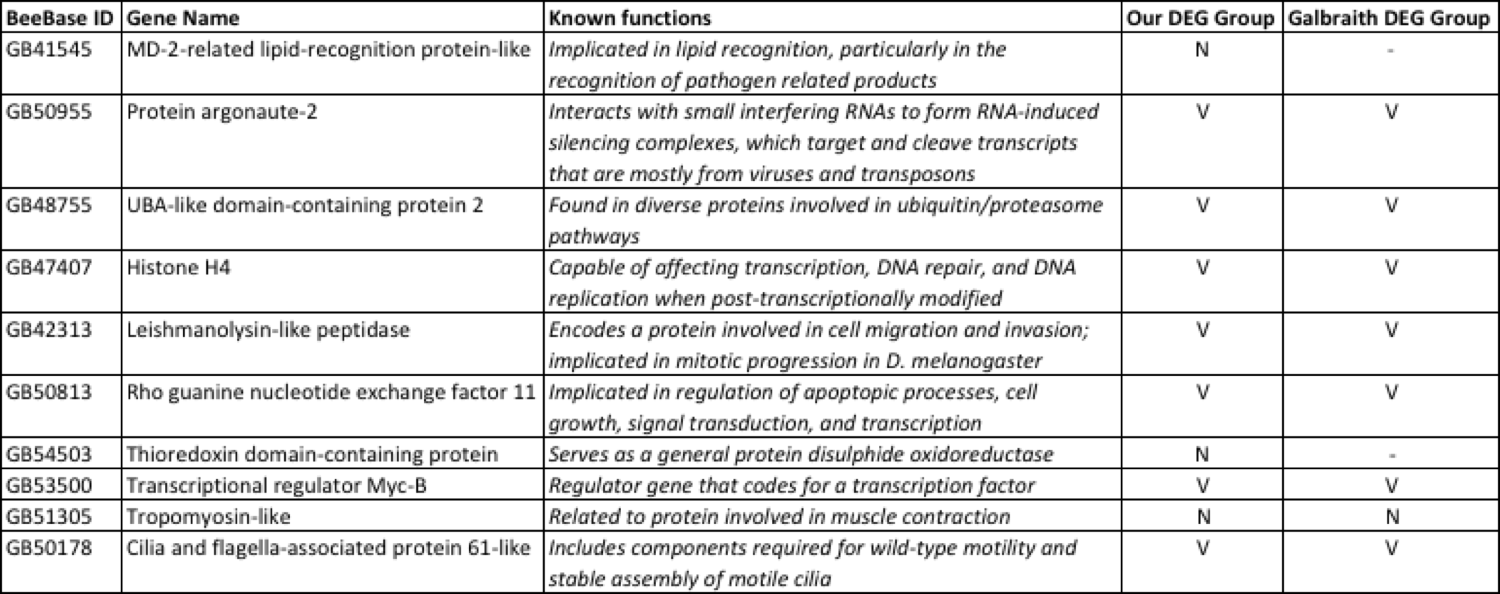
\includegraphics[width=\textwidth]{Images/virusGenes}
  \caption{Known functions of the mapped subset of 43 DEGs in the virus main effect of our study. Whether the gene was overrepresented in the virus or non-virus group is also indicated for both our study and the Galbraith study. Functionalities were extracted from Flybase, National Center for Biotechnology Information, and The European Bioinformatics Institute databases.}
  \label{tbl:virusGenes}
\end{table}

No interaction DEGs were observed between the diet and virus factors of the study, in any of the pipelines (DESeq2, edgeR, limma).

\subsection{Pairwise comparison of DEG results}

The number of DEGs across the six treatment pairings between the diet and virus factor ranged from 0 to 941 (Supplementary table \ref{tbl:pairDEGs}). Some of the trends observed in the main effect comparisons persisted: The diet level appeared to have greater influence on the number of DEGs than the virus level. Across every pair comparing the Chestnut and Rockrose levels, regardless of the virus level, the number of Chestnut-upregulated DEGs was higher than the number of Rockrose-upregulated DEGs (Supplementary table \ref{tbl:pairDEGs} C, D, E, F). For the pairs in which the diet level was controlled, the virus-exposed treatment showed equal to or more DEGs than the control treatment (Supplementary table \ref{tbl:pairDEGs} A, B). There were no DEGs between the treatment pair controlling for the control level of the virus effect (Supplementary table \ref{tbl:pairDEGs} A). These trends were observed for all three pipelines used (DESeq2, edgeR, and limma). 

\subsection{Comparison with Galbraith study}

We wished to explore the signal:to:noise ratio between the Galbraith dataset and our dataset. Basic MDS plots were constructed with the DESeq2 analysis pipeline, and we could immediately determine that the Galbraith dataset may better separate the infected and uninfected honey bees better than our dataset (Supplementary figure \ref{fig:mdsPlots}). We also noted that the first replicate of both treatment groups in the Galbraith data did not cluster as cleanly in the MDS plots. However, through this automatically-generated plot, we can only visualize information at the sample level. Wanting to learn more about the data at the gene level, we continued with additional visualization techniques.

We used parallel coordinate lines superimposed onto boxplots to visualize the DEGs associated with virus infection in the two studies. The background boxplot represents the distribution of all genes in the data, and each parallel coordinate line represents one DEG. To reduce overlapping of parallel coordinate lines, we often use hierarchical clustering techniques to separate DEGs into common patterns. See more information about this plotting method and the ideal visual structure of DEGs from chapter~\ref{sec:chapter2}.

We see that the 1,019 DEGs from the Galbraith dataset form relatively clean-looking visual displays (Figure \ref{fig:pcpGalbraith}). We do see that the first replicate of the virus group appears somewhat inconsistent with the other virus replicates in Cluster 2, confirming that this trend in the data that we saw in the MDS plot carried through into the DEG results. In contrast, we see that the 43 virus-related DEGs from our dataset do not look as clean in their visual displays (Figure \ref{fig:pcpRutterVirus}). The replicates appear somewhat inconsistent in their esimated expression levels and there is not always such a large difference between treatment groups. We see a similar finding when we also examine a larger subset of 1,914 diet-related DEGs from our study (Supplementary figure \ref{fig:pcpRutterDiet}). 

\begin{figure}[H]
\centering
% ../VirusHoneyBee/DESeq2/ClusterStandard/Clustering_data_FDR_05/
\begin{framed}
  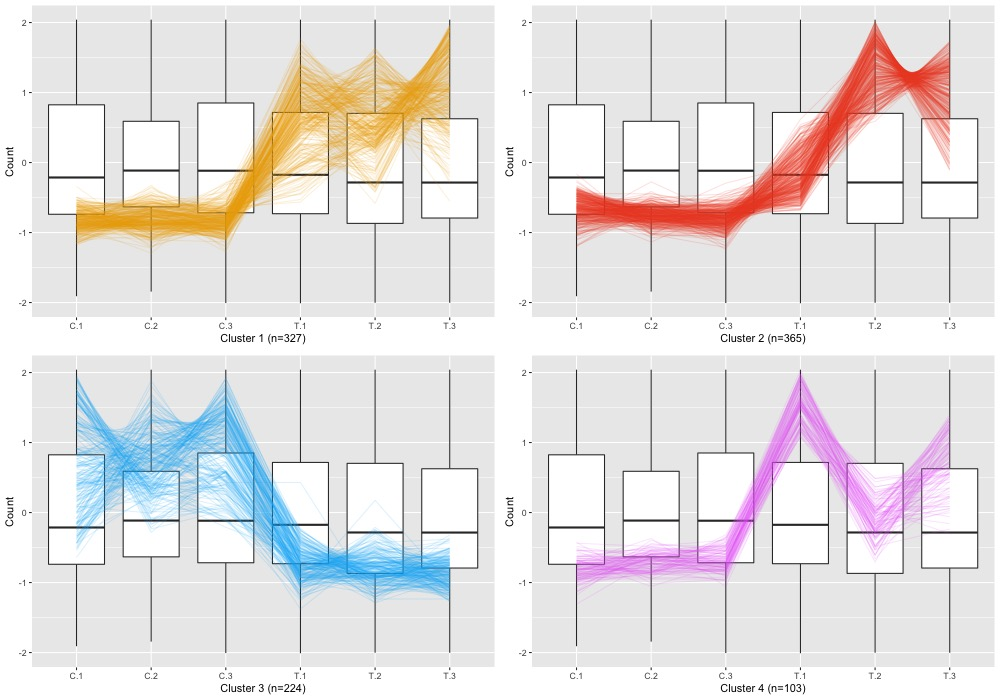
\includegraphics[width=\textwidth]{Images/C_T_4.jpg}
  \end{framed}
  \caption{Parallel coordinate plots of the 1,019 DEGs after hiearchical clustering of size four between the virus-infected and control groups of the Galbraith study. Here ``C'' represents control, and ``T'' represents treatment of virus. Clusters 1, 3, and 4 seem to represent DEGs that were overexpressed in the virus innoculated group, and Cluster 2 seems to represent DEGs that were overexpressed in the control group. In general, the DEGs appeared as expected, but there is rather noticeable deviation of the first replicate from the virus-treated sample (``T.1'') from the other virus-treated replicates in Cluster 2. Cluster 4 also has some inconsistent replicates across the virus-treated replicates.}
  \label{fig:pcpGalbraith}
\end{figure}

\begin{figure}[H]
\centering
% /../N_V/DESeq2/ClusterStandard/Clustering_data_FDR_05
\begin{framed}
  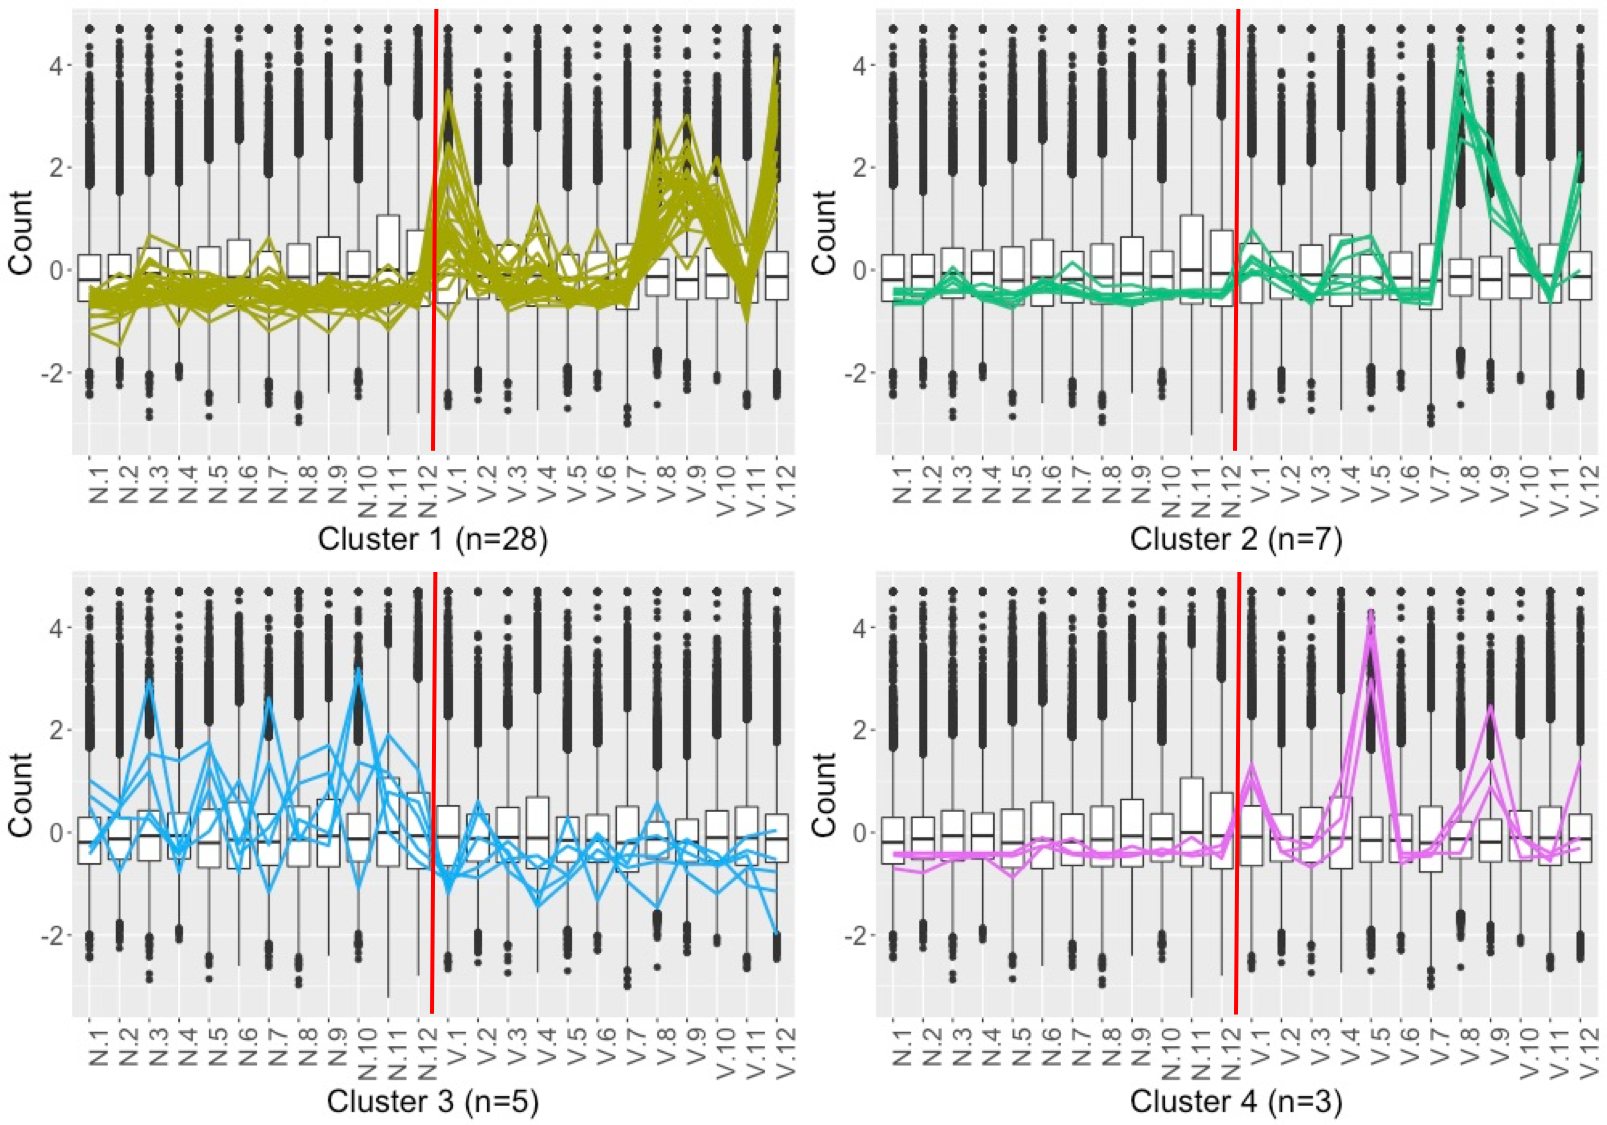
\includegraphics[width=\textwidth]{Images/N_V_4.png}
  \end{framed}
  \caption{Parallel coordinate plots of the 43 DEGs after hiearchical clustering of size four between the virus-infected and control groups of our study. Here ``N'' represents non-infected control group, and ``V'' represents treatment of virus. The vertical red line indicates the distinction between treatment groups. We see from this plot that the DEG designations for this dataset do not appear as clean compared to what we saw in the Galbraith dataset in Figure \ref{fig:pcpGalbraith}.}
  \label{fig:pcpRutterVirus}
\end{figure}

We also used litre plots to examine the structure of individual DEGs: We see that indeed the individual virus DEGs from our data (Supplementary figure \ref{fig:litreClusterRutter}) show less consistent replications and less differences between the treatment groups compared to the individual virus DEGs from the Galbraith data (Supplementary figures \ref{fig:litreCluster1} and \ref{fig:litreCluster2}). For the Galbraith data, we examined individual DEGs from the first cluster (Supplementary figure \ref{fig:litreCluster1}) and second cluster (Supplementary figure \ref{fig:litreCluster2}) because the second cluster had previously shown less consistency in the first replicate of the treatment group (figure \ref{fig:pcpGalbraith}). We verify this trend again in the litre plots with the DEG points in the second cluster showing less tight cluster patterns (Supplementary figures \ref{fig:litreCluster1} and \ref{fig:litreCluster2}).

Finally, we looked at scatterplot matrices to assess the DEGs. We created standardized scatterplot matrices for each of the four clusters (Figure \ref{fig:pcpGalbraith}) of the Galbriath data (Supplementary figures \ref{fig:GalbraithClust1SM}, \ref{fig:GalbraithClust2SM}, \ref{fig:GalbraithClust3SM}, and \ref{fig:GalbraithClust4SM}). We also created standardized scatterplot matrices for our data. However, as our dataset contained 24 samples, we would need to include 276 scatterplots in our matrix, which would be too numerous to allow for efficient visual assessment of the data. As a result, we created four scatterplot matrices of our data, each with subsets of 6 samples to be more comparable to the Galbraith data (Supplementary figures \ref{fig:RutterSM1}, \ref{fig:RutterSM2}, \ref{fig:RutterSM3}, and \ref{fig:RutterSM4}). We can again confirm through these plots that the DEGs from the Galbraith data appeared more as expected: Deviating more from the \textit{x=y} line in the treatment scatterplots while staying close to the \textit{x=y} line in replicate scatterplots.

Despite the virus-related DEGs (n = 1,019) from the Galbraith dataset displaying the expected patterns more than those from our dataset (n = 43), there was significant overlap (p-value < 2.2e-16) in the DEGs between the two studies (Supplementary figure \ref{fig:GRVenn}).

\subsection{Tolerance versus resistance}

Using the contrasts specified in Table \ref{tbl:contrasts}, we discovered 122 ``tolerance'' candidate genes and 125 ``resistance'' candidate genes. Within our 122 ``tolerance'' gene ontologies, we found functions related to metabolism (such as carbohydrate metabolism, fructose metabolism, and chitin metabolism). However, we also discovered gene ontologies related to RNA polymerase II transcription, immune response, and regulation of response to reactive oxygen species (Figure \ref{fig:revigo}A). Within our 125 ``resistance" gene ontologies, we found functions related to metabolism (such as carboyhydrate metabolism, chitin metabolism, oligosaccharide biosynthesis, and general metabolism) (Figure \ref{fig:revigo}B). 

\begin{figure}[H]
  \centering
  \begin{framed}
  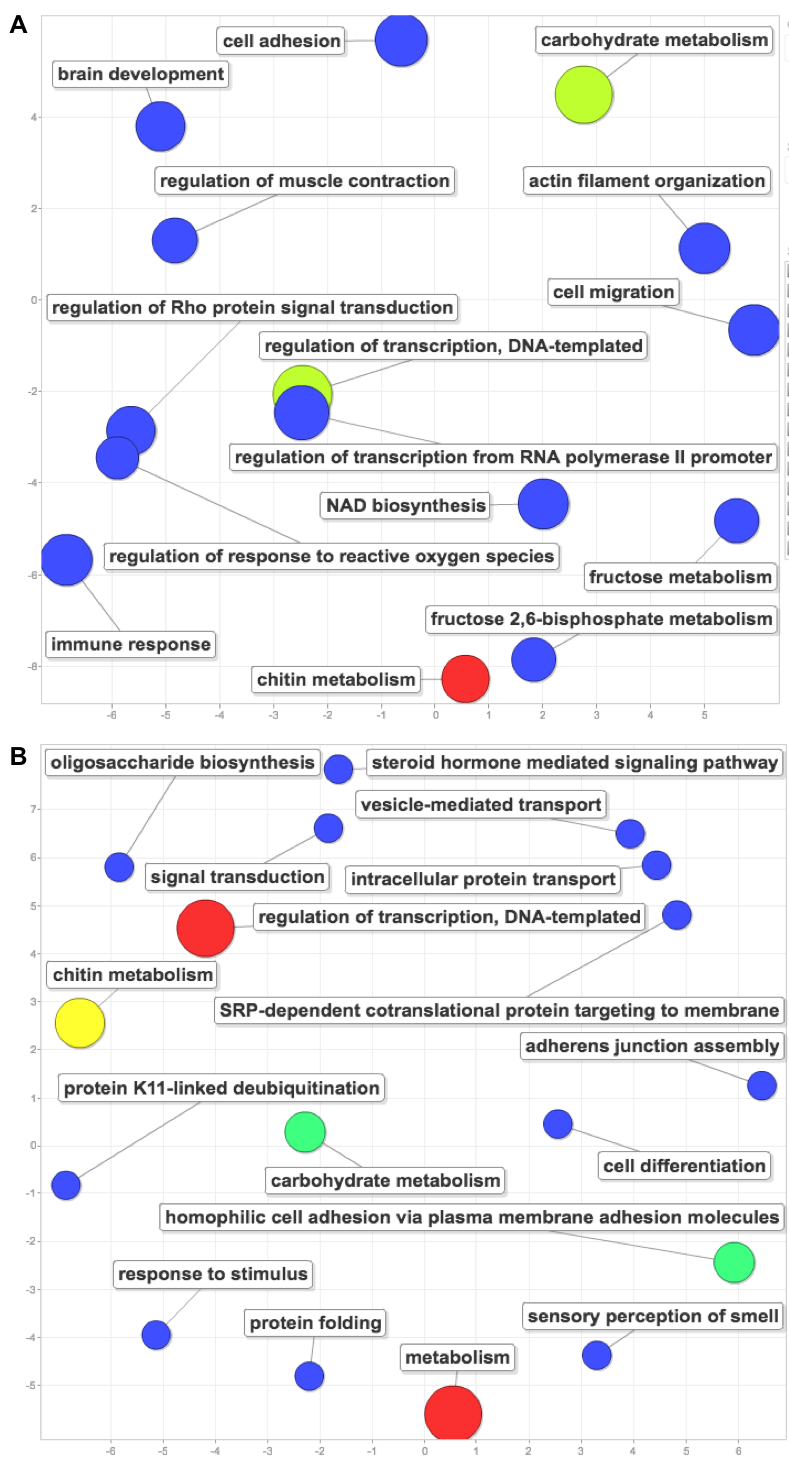
\includegraphics[width=0.8\textwidth]{Images/revigo}
  \end{framed}
  \caption{GO analysis results for the 122 DEGs related to our ``tolerance" hypothesis (A) and for the 125 DEGs related to our ``resistance" hypothesis (B).}
  \label{fig:revigo}
\end{figure}

\section{Discussion}

Challenges to honey bee health are a growing concern, in particular the combined, interactive effects of nutritional stress and pathogens (Dolezal and Toth 2018). In this study, we used RNA-sequencing to probe mechanisms underlying honey bee responses to two effects, diet quality and infection with the major virus of concern, IAPV. In general, we found a major nutritional transcriptomic response, with nearly 2,000 transcripts changing in response to diet quality (rockrose/poor diet versus chestnut/good diet). The majority of these genes were upregulated in response to high quality diet, and these genes were enriched for functions (Supplementary table \ref{tbl:ChestnutPathways}) such as nutrient signaling (insulin resistance) metabolism, and immune response (Notch signaling and JaK-STAT pathways). These data suggest high quality nutrition may allow bees to alter their metabolism, favoring investment of energy into innate immune responses.  

Somewhat surprisingly, the transcriptomic response to virus infection in our experiment was fairly limited. We found only 43 transcripts to be differentially expressed, some with known immune functions (Table \ref{tbl:virusGenes}) such as argonaute-2 and a gene with similarity to MD-2 lipid recognition protein, as well as additional genes related to transcriptional regulation, and muscle contraction. The small number of DEGs in this study may be partly explained by the large amount of noise in the data (Figure \ref{fig:pcpRutterVirus} and Supplementary figures \ref{fig:mdsPlots}B, \ref{fig:litreClusterRutter}, \ref{fig:RutterSM1}, \ref{fig:RutterSM2}, \ref{fig:RutterSM3}, and \ref{fig:RutterSM4}).

Given the noisy nature of our data, and our desire to hone in on genes with real expression differences, we compared our data to the Galbraith study (\citealt{galbraith}), which also examined bees response to viral infection. In contrast to our study, Galbraith et al. identified a large number of virus responsive trancripts, and generally had less noise in their data (Figure \ref{fig:pcpGalbraith} and Supplementary figures \ref{fig:mdsPlots}A, \ref{fig:litreCluster1}, \ref{fig:litreCluster2}, \ref{fig:GalbraithClust1SM}, \ref{fig:GalbraithClust2SM}, \ref{fig:GalbraithClust3SM}, and \ref{fig:GalbraithClust4SM}). To identify the most reliable virus-responsive genes from our study, we looked for overlap in the DEGs associated with virus infection on both experiments. We found a large, statistically significant (p-value < 2.2e-16) overlap, with 26/38 (68\%) of virus-responsive DEGs from our study also showing response to virus infection in Galbraith et al. (Supplementary figure \ref{fig:GRVenn}). This result gives us confidence that, although noisy, we were able to uncover consistent, replicable gene expression responses to virus infection with our data.  

Data visualization is a useful method to identify noise and robustness in RNA-seq data. In this study, we used extensive data visualization to improve the interpretation of our RNA-seq results. For example, the DESeq2 package comes with certain visualization options that are popular in RNA-sequencing analysis. One of these visualization is the multidimensional scaling (MDS) plot, which allows users to visualize the similarity between samples within a dataset. We could determine from this plot that indeed the Galbraith data may show more similarity between its replicates and differences between its treatments compared to our data (Supplementary figure \ref{fig:mdsPlots}). However, the MDS plot only shows us information at the sample level. We wanted to investigate how these differences in the signal:to:noise ratios of the datasets would affect the structure of any resulting DEGs. As a result, we also used three plotting techniques from the bigPint package: We investigated the 1,019 virus-related DEGs from the Galbraith dataset and the 43 virus-related DEGs from our dataset using parallel coordinate lines, litre plots, and scatterplot matrices. To prevent overlapping issues in our plots, we used a hierarchical clustering technique for the parallel coordinate lines to separate the set of DEGs into smaller groups. We also needed to examine four subsets of samples from the Galbraith dataset to make effective use of the scatterplot matrices. After these tailorizations, we determined that the same patterns we saw in the MDS plots regarding the entire dataset extended down the pipeline analysis into the DEG calls: Even the DEGs from the Galbraith dataset showed more similarity between their replicates and differences between their treatments compared to those from our data. However, the 365 DEGs from the Galbraith data in Cluster 2 of Figure \ref{fig:pcpGalbraith} showed an inconsistent first replicate in the treatment group (``T.1''), which was something we observed in the MDS plot. This indicates that this feature also extended down the analysis pipeline into DEG calls. We believe these visualization applications can be useful for future researchers analyzing RNA-sequencing data to quickly and effectively ensure that the DEG calls look reliable or at least overlap with DEG calls from similar studies that look reliable. We also expect this type of visualization exploration can be especially crucial when studying complex organisms that do not have genetic identicalness or similarity between replicates and/or when using experiments that may lack rigid design control.

One of the goals of this study was to use our RNA-seq data to assess whether transcriptomic responses to diet quality and virus infection provide insight into whether high quality diet can buffer bees from pathogen stress via mechanisms of ``resistance'' or ``tolerance''. Recent evidence has suggested that overall immunity is determined by more than just ``resistance'' (the reduction of pathogen fitness within the host by mechanisms of avoidance and control) (\citealt{resTol2}). Instead, overall immunity is related to ``resitance'' in conjunction with ``tolerance'' (the reduction of adverse effects and disease resulting from pathogens by mechanisms of healing) (\citealt{resTol1}, \citealt{resTol2}). Immune-mediated resistance and diet-driven tolerance mechanisms are costly and may compete with each other (\citealt{resTol1}, \citealt{resTol4}). Data and models have suggested that selection can favor an optimum combination of both resistance and tolerance (\citealt{resTol5}, \citealt{resTol6}, \citealt{resTol7}, \citealt{resTol8}). We attempted to address this topic through specific gene expression contrasts (Table \ref{tbl:contrasts}), accompanied by GO analysis of the associated gene lists. We found an approximately equal number of resistance (n = 125) and tolerance (n = 122) related candidate genes, suggesting both processes may be playing significant roles in dietary buffering from pathogen induced mortality. Resistance candidate genes had functions related to several forms of metabolism (chitin and carbohydrate), regulation of transcription, and cell adhesion. Tolerance candidate genes had functions related to carbohydrate metabolism and chitin metabolism. However, they also showed functions related to immune response (Figure \ref{fig:revigo}A).

Overall, these data suggest complex transcriptomic responses to multiple stressors in honey bees. Diet has the potential for large and profound effects on transcriptional responses in honey bees, and differences in diet may set up the potential for both resistance and tolerance to virus infection. Moreover, this study in general also demonstrated the possible benefits of using data visualizations and multiple datasets to address inherently messy biological data. For instance, by verifying the subsantial overlap in our DEG lists to those obtained in another study that addressed a similar question but in a more controlled manner, we were able to place much higher confidence in the differential gene expression results from our otherwise noisy data. We hope these results underline the need for researchers to use data visualization techniques to understand and interpret RNA-sequencing datasets.

\section{Acknowledgments}

This project was an effort between Adam Dolezal, Amy Toth, Dianne Cook, and myself.

%%%%%%%%%%%%%%%%%%%%%%%%%%%%%%%%%%%%%%%%%%%%%%%%%%%%%%%%%%%%%%%%%%%%%%%%%%%%%%%%%%%%%%%
%%%%%%%%%%%%%%%%%%%%%%%%%%%%%%%%%%%%%%%%%%%%%%%%%%%%%%%%%%%%%%%%%%%%%%%%%%%%%%%%%%%%%%%

\chapter{Conclusions}

Data visualization of large biological datasets is an expanding field in recent years. There is growing recognition that as large and complex datasets become more accessible, effective tools to extract meaningful knowledge from them becomes more vital. There is also growing evidence that the most reliable results from analyzing such datasets comes from an analysis that incorporates traditional models and visualizations in an iterative fashion. The research in this dissertation has demonstrated useful contributions to large biological data visualization in, specifically in regards to genealogical and gene expression applications. 

\section{Contribution to genealogical data visualization}

Our most novel contribution to the visualization of large genealogical datasets is our plot that allows users to view the ancestors and descendants of a given variety with the horizontal axis constrained so that the further from the center that a variety is located, the more generations that variety is distanced from the centered variety of interest. This plotting technique is unique because most genealogical visualization software do not allow for labels to be repeated, which can cause conflicts when relationships are formed between generations and given individuals subsequently may contain multiple (ambiguous) generation count separations from other individuals in their lineage. We demonstrated the problem using a soybean dataset. Our plotting method that solved this problem \code{plotAncDes()} was shared and published in our open source software publication \pkg{ggenealogy}. Another useful contribution that we made to the visualization of large genealogical datasets is our plot that superimposes genealogical paths of interest across an entire lineage. We effectively constructed an algorithm that reduces the text overlap between the labels of such a plot. Again, our plotting method that mitigated this problem \code{plotPathOnAll()} was shared and published in our open source software publication \pkg{ggenealogy}. Both of these novel plotting techniques were discussion in chapter~\ref{sec:chapter1}.

\section{Contribution to RNA-sequencing data visualization}

We made several important contributions to the visualization of RNA-sequencing datasets. Chapter~\ref{sec:chapter2} served as a case in point regarding the need for effective visualization techniques in RNA-sequencing studies. Specifically, we provided several real-world examples where data visualization tools were able to detect issues with the data and/or the model that was applied that could be used to successfully redirect users to either clean the data or apply a new model. For instance, we demonstrated that our visual techniques could quickly indicate that a publicly-available dataset containing technical replicates of liver and kidney RNA samples required more than library size scaling and that it benefited from TMM normalization \citep{Marioni}. Likewise, we demonstrated that a publicly-available RNA-sequencing dataset of Saccharomyces cerevisiae (yeast) grown in YP-Glucose required between lane normalization and not just within lane normalization using our graphical methods \cite{Risso}. We plan to publish similar work to what was presented in chapter~\ref{sec:chapter2} and believe that our collection of easy-to-follow examples that underline the importance of using effective visualization tools when analyzing RNA-sequencing may play a small but important part in influencing scientists who perform RNA-sequencing studies to incorporate such practice within their usual analysis pipelines.

In chapter~\ref{sec:chapter3}, we also provided important contributions to the field of RNA-sequencing analysis because we discussed the technology behind the effective visualization tools that we created and demonstrated to have been of importance back in chapter~\ref{sec:chapter2}. One technology tool we introduced that is not common in data visualization for RNA-sequencing is the application of an interactive foreground superimposed onto a static background. We leveraged this relatively new technology to develop our plotting techniques to superimpose a gene of interest (usually a DEG from a model) onto a static background of all genes within the dataset. This technology allows users to quickly sift through a subset of genes (say a DEG list produced from a model) and determine how they overlay across the whole dataset, thereby assessing whether its replicate consistency and treatment variability seems reasonable for a DEG designation. We plan to publish a clear and intuitive vignette that explains how users can create and explore interactive scatterplot matrices, litre plots, and parallel coordinate plots easily into their usual analysis pipelines, especially because we created our software tools to be easily incorporable into popular RNA-sequencing analysis software (\citealt{deseq2}, \citealt{edger}, \citealt{limma}). We also plan to publish the software as an open source package called \pkg{bigPint} onto Bioconductor. We hope that such efforts will again serve a small but meaningful role in influencing scientists to use such visualization techniques during their usual RNA-sequencing analysis pipelines.

As part of our work in chapter~\ref{sec:chapter4}, we performed detailed comparative visualization analyses that may be useful for biologists working with inherently messy RNA-sequencing data. Specifically, we examined honey bees from polyandrous colonies, while a previous study examined honey bees from single-drone colonies (\citealt{galbraith}). As a consequence, the honey bees in our study had about 25\% genetic identicalness, whereas the honey bees from the other study had about 75\% genetic identicalness (\citealt{sisters}). Using the graphical techniques we developed and introduced in chapters~\ref{sec:chapter2} and ~\ref{sec:chapter3}, we discovered that our DEGs did not appear clean in terms of replicate consistency and treatment differentiation, whereas the DEGs from the other study did. Despite the noticeable visual differences in the signal:to:noise ratios between the two studies, we found subsantial overlap in the DEG lists between our study and their study, and hence were able to place much higher confidence in the DEG results from our otherwise noisy data.

We believe our visualization methodology here that compared the two studies was unique and can be used as an example for scientists who work with datasets that may have low signal:to:noise ratios. In some cases, there are tradeoffs between controlled experimental designs and effective simulation of real-world observations: For example, while our dataset was less genetically controlled, it reflected the phenomenon we were studying given that honey bees are naturally polyandrous (\citealt{patriline}). 

In contrast, the other study offered more genetic control, but did not reflect the typical honey bee genotypic variance seen in colonies seeing that single-drone colonies tend to be less healthy (\citealt{geneticDiverse}). In other words, while it is justifiable for us to use polyandrous colonies in our study to more accurately reflect most healthy colonies, we should accept that our signal:to:noise ratio may consequentely be low and may decide to compare our DEG lists with studies assessing the same variables under more controlled conditions, especially if we can quickly verify visually that their signal:to:noise ratio is respectfully higher. This careful technique that may result in more reliable results can be easily employed with our plotting tools, as we showed.

\section{Contribution to understanding how diet quality and viral innolcuation affect gene expression in honey bees}

As far as we know, before our study in chapter~\ref{sec:chapter4}, there were few to no studies investigating honey bee gene expression patterns specifically related to monofloral diets, and few to no studies investigating honey bee gene expression patterns related to the combined effects of diet in any broad sense and viral innoculation in any broad sense. There is also scarce information about whether the protective effect of good diet in honey bees is due to direct effects on immune function (resistance), or if it is due to indirect effects of energy availability (tolerance). We attempted to address this question through gene expression contrasts, and found a similar number of resistance (n = 125) and tolerance (n = 122) related candidate genes, suggesting both processes may serve roles in the dietary buffering of honey bees from pathogenic infection. We also discovered that tolerance candidate genes had functions related to carbohydrate metabolism, chitin metabolism, immune response, and regulation of transcription, whereas resistance candidate genes had functions related to several forms of metabolism (chitin and carbohydrate), regulation of transcription, and cell adhesion.

\section{Future work}

The \pkg{ggenealogy} package could be improved in several ways. First, we could employ Shiny applications. The reactive programming could save users of \pkg{ggenealogy} the time of using command line for each change of input as well as the inefficiency of rerunning code. It could also enhance the interactivity. A Shiny application that uses certain \pkg{ggenealogy} functionality is already available for users who wish to explore the soybean genealogy; the data can be viewed at \url{http://shiny.soybase.org/CNV/}. Second, we could incorporate plotting tools that examine not only quantitative variables (such as our example variable of "year"), but also categorical variables associated with individuals in datasets. Third, the \pkg{ggenealogy} visualization tool \code{plotPathOnAll()} is suitable as a data exploration tool, but not always as a publication tool. This is because we still see textual overlap in datasets that are small enough to - in theory - be represented with all labels in a readable format (see Figure \ref{fig:plotTNBin6}). As such, an addition of a feature to the package that allows users to manually fine-tune automated plots could be useful. Fourth, the \pkg{ggenealogy} package could tested on additional genealogical data sets. Exploring several datasets with the software would allow us to fix remaining bugs, and provide us further insight into how to make our tools available for a wide range of data input formats. 

The \pkg{bigPint} package could also be improved in several ways. First, the speed of the interactivity could be increased. As the number of samples and/or genes increases, the speed can become noticeably slower and can sometimes render the interactive plotting tools ineffective. Second, we still have issues of data overlapping which could be addressed through additional plotting techniques. Third, we could continue to explore examples of how these plotting techniques can lead to more reliable analyses and conclusions among RNA-sequencing studies. The development of additional examples could add more persuasion for scientists to employ visualization techniques in their usual analysis pipelines.

It may also be of interest to conduct additional comparisons between well-controlled but artifical and uncontrolled but realistic RNA-sequencing study designs, similar to what we did in chapter~\ref{sec:chapter4}. Given that many biologists choose to collect data that has less control in their experimental design in order to maintain generalizability of their results, it may be useful to better understand how the DEGs from such environmental designs appear and how often the DEG lists overlap between differing experimental designs. All of this can add confidence to the reliability of results from RNA-sequencing studies while also familiarizing scientists with visualization approaches for gene expression analysis.


%%%%%%%%%%%%%%%%%%%%%%%%%%%%%%%%%%%%%%%%%%%%%%%%%%%%%%%%%%%%%%%%
%%%%%%%%%%%%%%%%%%%%%%%%%%%%%%%%%%%%%%%%%%%%%%%%%%%%%%%%%%%%%%%%

\chapter{Supplementary material for Chapter 3}
\label{sec:suppchapter2}

This file contains supplementary analyses that the reader might find useful, and that extend upon several of the main concepts discussed in chapter \ref{sec:chapter2}. We include additional examples of how parallel coordinate plots, scatterplots matrices, and litre plots can be used to assess normalization and DEG calls. Below we provide a brief description of the first seven figures in this supplementary section:

\begin{itemize}

\item Figure~\ref{sbIRClusters} shows parallel coordinate plots of hierarchical clusters in a similar manner as Figure~\ref{sbIRClustersSig} in chapter \ref{sec:chapter2}. The data comes from the iron-metabolism soybean study, and has been filtered and standardized. However, unlike Figure~\ref{sbIRClustersSig} in chapter \ref{sec:chapter2} only showing significant genes, Figure~\ref{sbIRClusters} here shows all genes.

\item Figures~\ref{sbIRClusterSigSM1} through~\ref{sbIRClusterSigSM4} show scatterplot matrices of the significant genes in the iron-metabolism soybean dataset for each of the four clusters that resulted from hiearchical clustering analysis. They provide an additional and complementary perspective on these DEG calls from what we saw with the parallel coordinate plots in Figure~\ref{sbIRClusters}. 

\item Figure~\ref{mdsSwitch} shows that some of the most popular RNA-seq visualization tools cannot always detect common errors, such as sample switching. Side-by-side boxplots and MDS plots are shown for the soybean cotyledon dataset after deliberately switching samples between treatment groups. For the most part, they are unable to detect the error. In contrast, the less-popular method of scatterplot matrices can quickly detect the possibility of the error (see Figure~\ref{sbCNSwitchedSM} from chapter \ref{sec:chapter2}).

\item Figure~\ref{litreCluster1} shows example litre plots for two significant genes from Cluster 1. The reader may wish to view it alongside Figure~\ref{repDot} from chapter \ref{sec:chapter2}, which contains example litre plots for significant genes from Clusters 2, 3, and 4.

\end{itemize}

The last twenty figures in the supplementary section are all related to the application of normalization techniques to the liver and kidney technical replicate data that were introduced in chapter \ref{sec:chapter2}. These figures also introduce examples that demonstrate the effect of standardizing data before viewing them. A brief description of these twenty figures starts on Page 9.

%%%%%%%%%%%%%%%%%%%%%%%%%%%%%
%%%%%%%%%%%%%%%%%%%%%%%%%%%%%
%%%%%%% Begin Figures %%%%%%% 
\null
\begin{figure}[t!]
\begin{framed}
\centerline{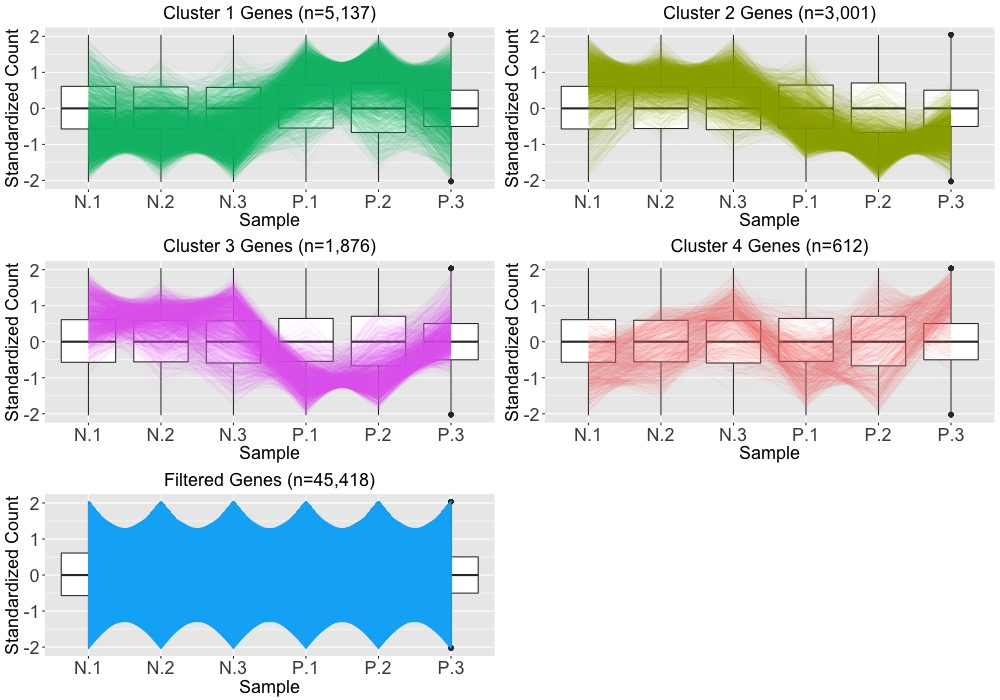
\includegraphics[width=\columnwidth]{MakeFigures/sbIRClusters.jpg}}
\end{framed}
\caption{Example application of parallel coordinate plots using the iron-metabolism soybean dataset. We filtered genes with low means and/or variance, performed a hierarchical clustering analysis with a cluster size of four, and visualized the results using parallel coordinate lines. Most non-filtered genes were in Clusters 1 and 2, which both showed overexpression in one treatment and underexpression in the other treatment. The genes in Cluster 4 mostly showed messy patterns with low signal to noise ratios. Interestingly, Cluster 3 looked similar to Cluster 2 (large values for group N and small values for group P), except for unexpectedly large values for the third replicate of group P.
\label{sbIRClusters}}
\end{figure}

\clearpage
\null
\begin{figure}[t!]
\begin{framed}
\centerline{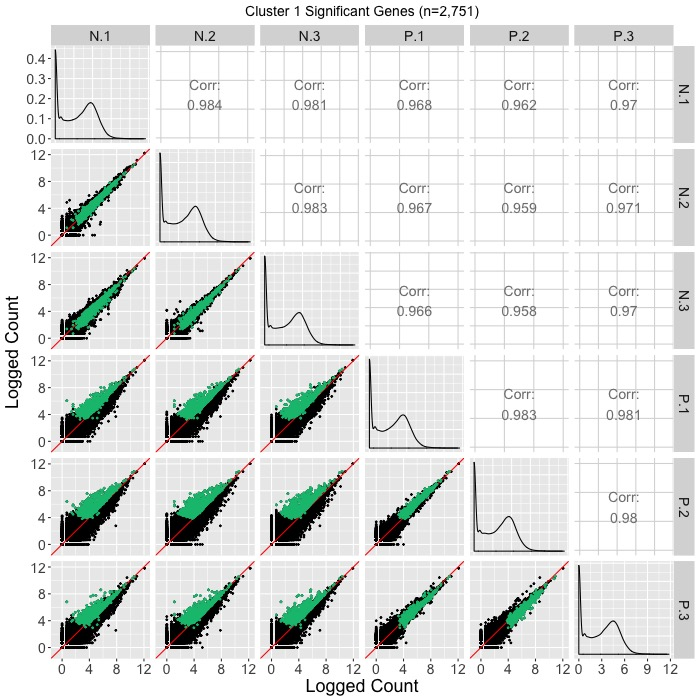
\includegraphics[width=\columnwidth]{MakeFigures/sbIRClusterSigSM1.jpg}}
\end{framed}
\caption{Example of using a scatterplot matrix to assess DEG calls from a model in the iron-metabolism soybean dataset. There were 2,751 significant genes in Cluster 1 after performing a hierarchical clustering analysis with a cluster size of four (Figure~\ref{sbIRClustersSig} in chapter \ref{sec:chapter2}). These significant genes are overlaid in green on the scatterplot matrix. They follow the expected patterns of differential expression with most green points falling along the \textit{x=y} line in the scatterplots between replicates, but deviating from the \textit{x=y} line in the scatterplots between treatments. The deviation consistently demonstrates higher expression in the P group than in the N group. Hence, these green points seem to represent genes that were significantly overexpressed in the P group, which draws the same conclusion with what we derived using the parallel coordinate plots in Figure~\ref{sbIRClustersSig} of chapter \ref{sec:chapter2}. One difficulty with plotting such a large number of DEGs onto the scatterplot matrix is that overplotting can obscure our inability to determine how many DEGs are in a given location. This is why we might also view these genes individually in litre plots (Supplementary Figure~\ref{litreCluster1}).
\label{sbIRClusterSigSM1}}
\end{figure}

\begin{figure}[t!]
\begin{framed}
\centerline{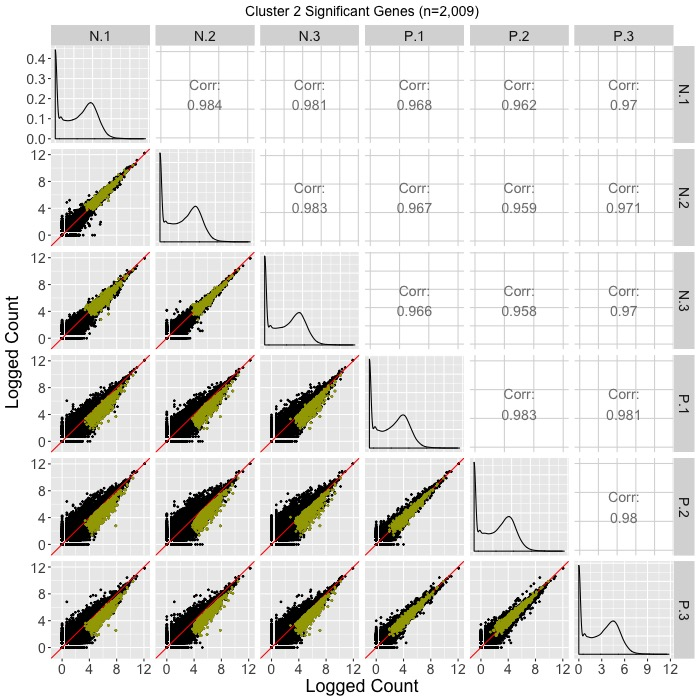
\includegraphics[width=\columnwidth]{MakeFigures/sbIRClusterSigSM2.jpg}}
\end{framed}
\caption{Example of using a scatterplot matrix to assess DEG calls from a model in the iron-metabolism soybean dataset. There were 2,009 significant genes in Cluster 2 after performing a hierarchical clustering analysis with a cluster size of four (Figure~\ref{sbIRClustersSig} in chapter \ref{sec:chapter2}). These significant genes are overlaid in mustard on the scatterplot matrix. They follow the expected patterns of differential expression with most mustard points falling along the \textit{x=y} line in the scatterplots between replicates, but deviating from the \textit{x=y} line in the scatterplots between treatments. The deviation consistently demonstrates higher expression in the N group than in the P group. Hence, these mustard points seem to represent genes that were significantly overexpressed in the N group, which draws the same conclusion with what we derived using the parallel coordinate plots in Figure~\ref{sbIRClustersSig} of the paper. One difficulty with plotting such a large number of DEGs onto the scatterplot matrix is that overplotting can obscure our inability to determine how many DEGs are in a given location. This is why we might also view these genes individually in litre plots (Figure~\ref{repDot} A and B in chapter \ref{sec:chapter2}).
\label{sbIRClusterSigSM2}}
\end{figure}
  

\begin{figure}
\begin{framed}
\centerline{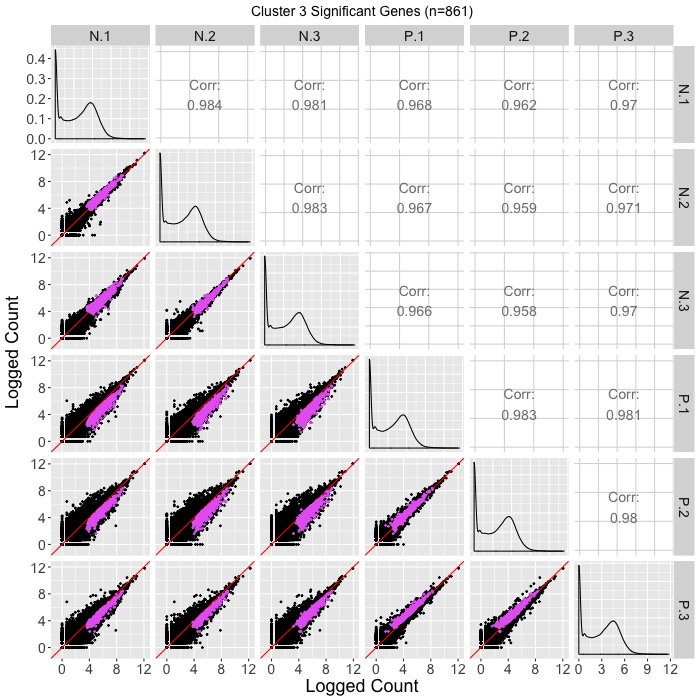
\includegraphics[width=\columnwidth]{MakeFigures/sbIRClusterSigSM3.jpg}}
\end{framed}
\caption{Example of using a scatterplot matrix to assess DEG calls from a model in the iron-metabolism soybean dataset. There were 861 significant genes in Cluster 3 after performing a hierarchical clustering analysis with a cluster size of four (Figure~\ref{sbIRClustersSig} in chapter \ref{sec:chapter2}). These significant genes are overlaid in pink on the scatterplot matrix. For the most part, they follow the expected patterns of differential expression with pink points falling along the \textit{x=y} line in the scatterplots between replicates, but deviating from the \textit{x=y} line in the scatterplots between treatments. The deviation consistently demonstrates higher expression in the N group than in the P group. However, the scatterplot between replicates P.1 and P.3 shows slightly higher expression in P.3, and the scatterplot between replicates P.2 and P.3 also shows slightly higher expression in P.3. Hence, these pink points seem to represent genes that were significantly overexpressed in the N group, but with slight inconstencies in the replicates in the P group. The parallel coordinate plots in Figure~\ref{sbIRClustersSig} of the paper showed this same conclusion and perhaps more clearly. One difficulty with plotting such a large number of DEGs onto the scatterplot matrix is that overplotting can obscure our inability to determine how many DEGs are in a given location. This is why we might also view these genes individually in litre plots (Figure~\ref{repDot} C and D in chapter \ref{sec:chapter2}).
\label{sbIRClusterSigSM3}}
\end{figure}  

\clearpage
\null
\begin{figure}[t!]
\begin{framed}
\centerline{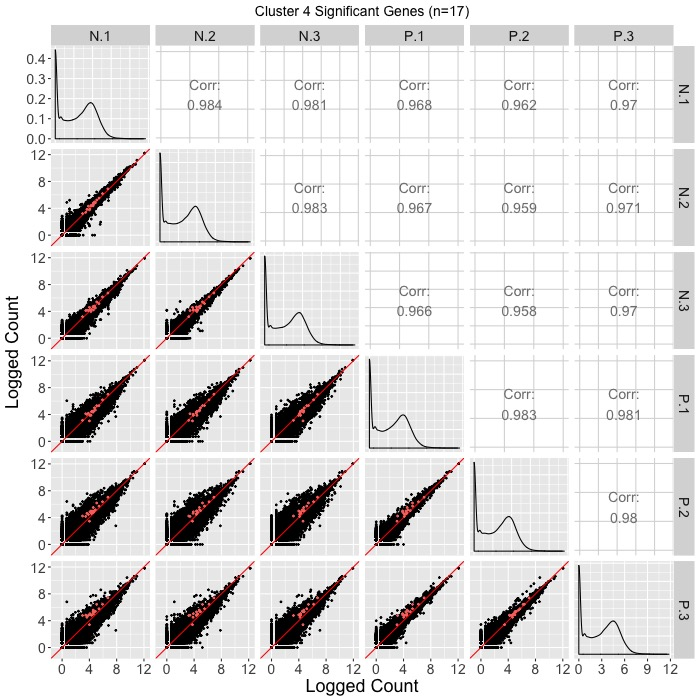
\includegraphics[width=\columnwidth]{MakeFigures/sbIRClusterSigSM4.jpg}}
\end{framed}
\caption{Example of using a scatterplot matrix to assess DEG calls from a model in the iron-metabolism soybean dataset. There were 17 significant genes in Cluster 4 after performing a hierarchical clustering analysis with a cluster size of four (Figure~\ref{sbIRClustersSig} in chapter \ref{sec:chapter2}). These significant genes are overlaid in coral on the scatterplot matrix. For the most part, they do not seem to follow the expected patterns of differential expression: In many of the scatterplots between treatments, the coral points do not seem to deviate much from the \textit{x=y} line. Moreover, in the scatterplots between P.1 and P.2 as well as P.1 and P.3, the coral points seems to indicate an underexpression of the P.1 replicate. We similarly saw somewhat messy looking DEG calls in Cluster 4 in the form of parallel coordinate plots (Figure~\ref{sbIRClustersSig} of chapter \ref{sec:chapter2}) and litre plots (Figure~\ref{repDot} E and F of chapter \ref{sec:chapter2}).
\label{sbIRClusterSigSM4}}
\end{figure}  

\clearpage
\null
\begin{figure}[!t]
\centerline{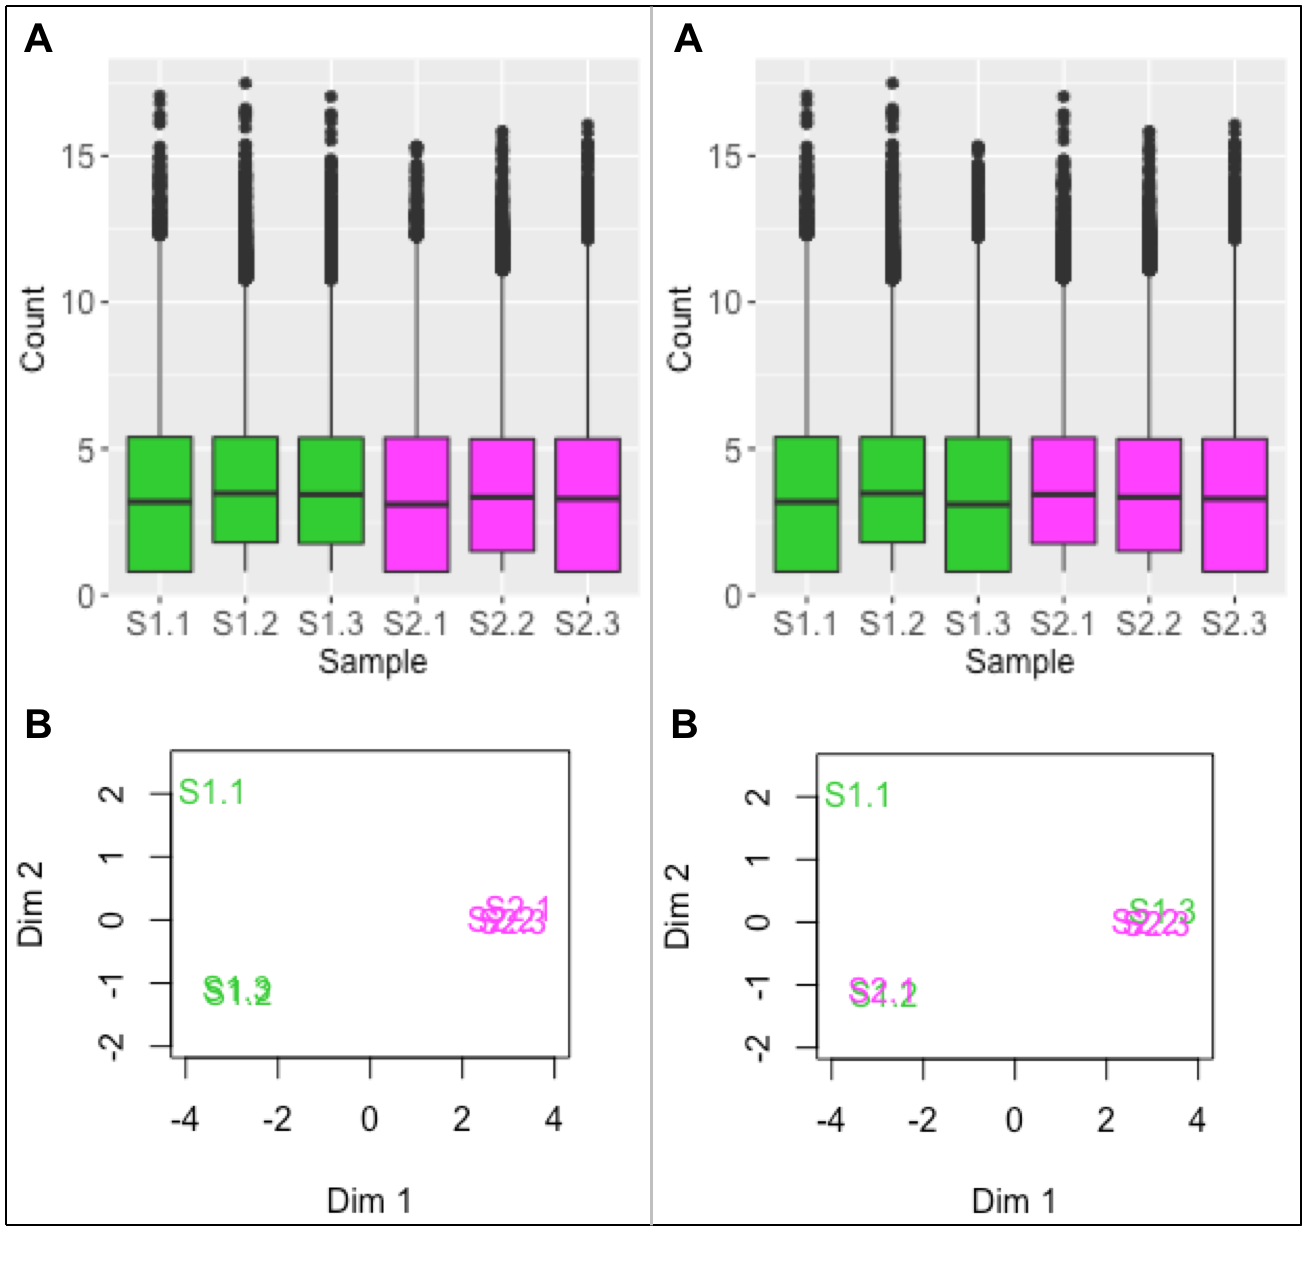
\includegraphics[width=0.7\columnwidth]{MakeFigures/mdsSwitch.png}}
\caption{Boxplots and MDS plots are popular plotting tools for RNA-seq analysis. This figure shows these traditional visualization methods applied to the soybean cotyledon data before sample switching (left half) and after sample switching (right half). We cannot suspect from the right boxplot that samples S1.3 and S2.1 have been swapped (subplots A). This is because all six samples have similar five number summaries. For the MDS plots, we do see a cleaner separation of the two treatment groups across the first dimension in the left plot than in the right plot (subplots B). However, taking into account the second dimension, both MDS plots contain three clusters, with sample S1.1 appearing in its own cluster. Without seeing one distinct cluster for each of the two treatment groups, it is difficult to suspect that samples S1.3 and S2.1 have been swapped in the right MDS plot (subplots B). We can only derive clear suspicion that the samples may have been switched by using less-popular plots that provide gene-level resolution like with the scatterplot matrix from Figure~\ref{structure} in chapter \ref{sec:chapter2}.
\label{mdsSwitch}}
\end{figure}

\clearpage
\null 
\begin{figure}[t!]
\begin{framed}
\centerline{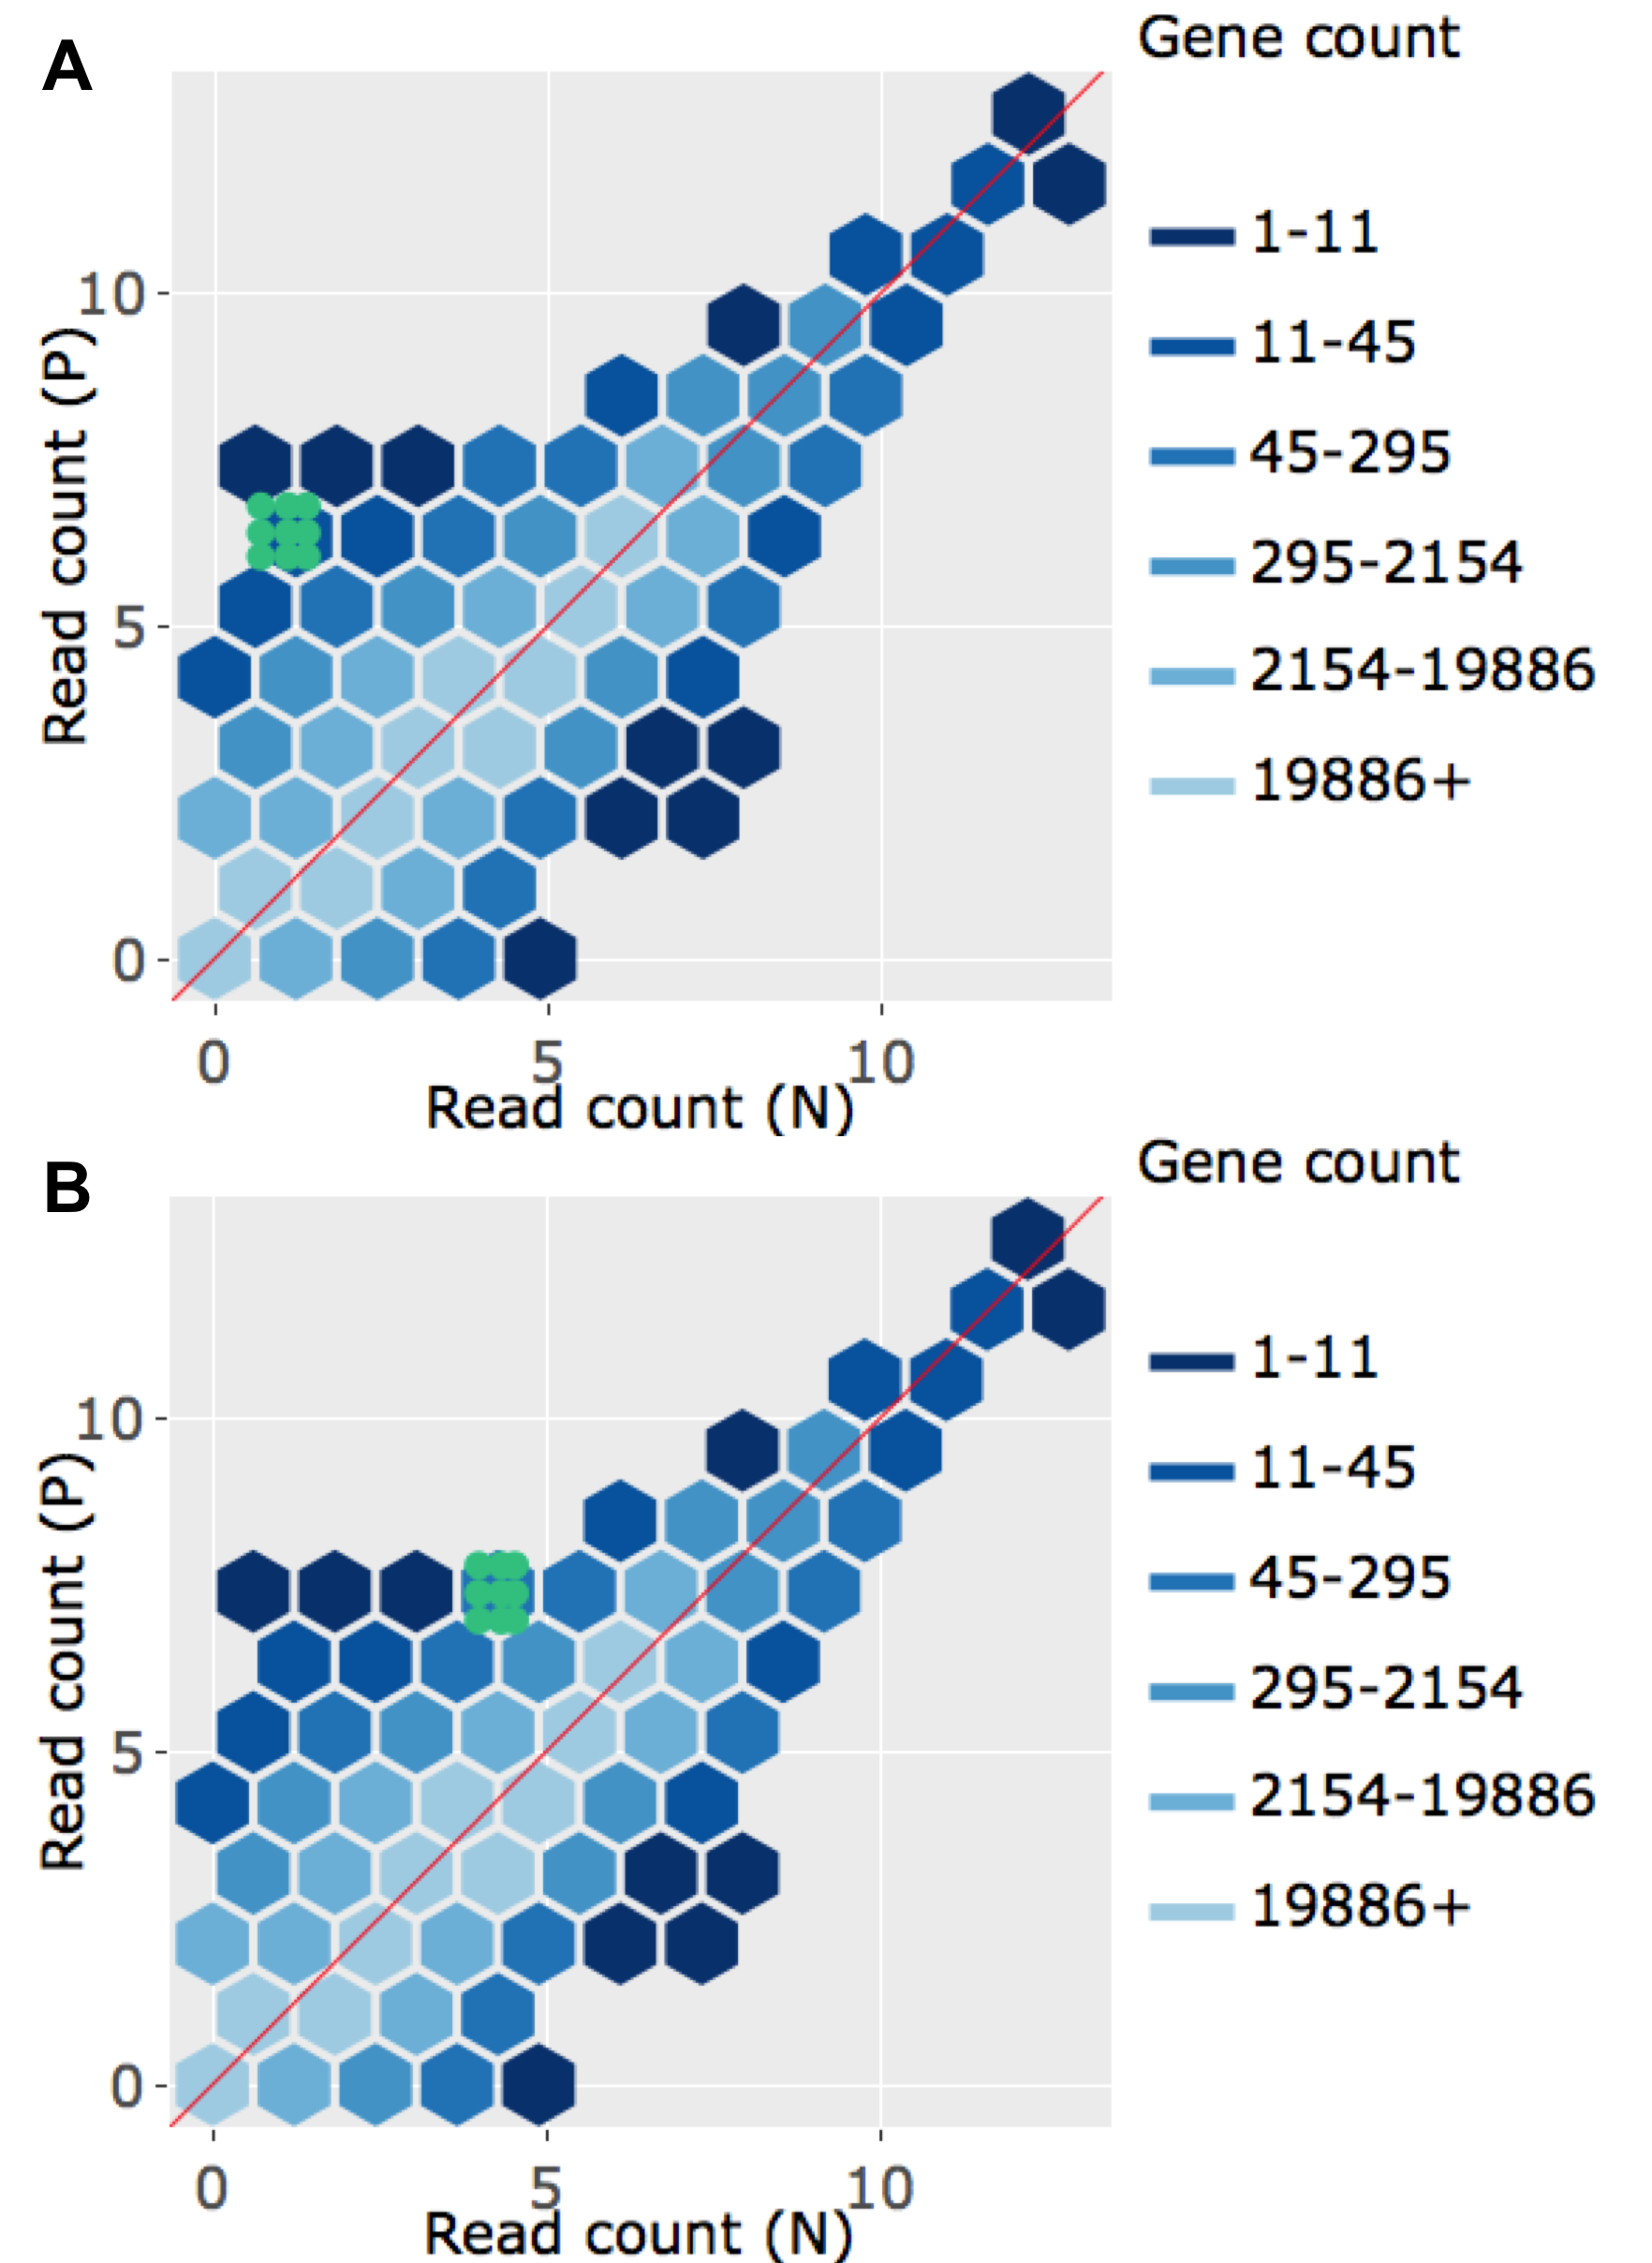
\includegraphics[width=0.7\columnwidth]{MakeFigures/Dashboards/litreCluster1/litreCluster1.jpg}}
\end{framed}
\caption{Litre plots for significant genes inside Cluster 1 from Figure~\ref{sbIRClustersSig} of the paper. Subplots A and B each overlay an example significant gene as nine green points. The genes show patterns expected of differentially-expressed ones, by clumping together and deviating from the \textit{x=y} line. Moreover, the genes appear over-expressed in the P group. This is consistent with what we saw in the parallel coordinate plots of Figure~\ref{sbIRClustersSig} from chapter \ref{sec:chapter2}. To interactively view the litre plot for all significant genes within Cluster 1, please visit https://rnaseqvisualization.shinyapps.io/litreCluster1.
\label{litreCluster1}}
\end{figure}   

\clearpage
The rest of the figures in this supplementary section (Figures~\ref{lkClustersKeep} through~\ref{litreClusterAdd-St}) provide additional examples related to the closing case study introduced in chapter ~\ref{sec:chapter2}. In this case study, technical replicates of kidney and liver RNA-seq data was initially analyzed using library scale normalization. This process lead to 7,050 kidney DEGs and 1,968 liver DEGs, but subsequent visualization analysis suggested that a subset of the kidney DEGs may be unreliable (Figure~\ref{lkClusters}A from chapter \ref{sec:chapter2}). Upon reviewing the geometrical structure of the data in the form of a scatterplot matrix, a subset of overexpressed liver genes was discovered, implicating the need for a more rigorous form of normalization (Figure~\ref{lkSM} from chapter \ref{sec:chapter2}). As a result, TMM normalization was then applied to the data, which lead to 3,974 kidney DEGs and 3,546 liver DEGs. Ensuing visualization analysis verified that these DEGs now appeared more reliable (Figure~\ref{lkClusters}B from chapter \ref{sec:chapter2}). \\

In the remaining figures of this supplementary file, we thoroughly explore four subsets of genes from this case study in the form of parallel coordinate plots, scatterplot matrices, and litre plots. We also use variants of some of the techniques introduced in chapter \ref{sec:chapter2}. Namely, we demonstrate the use of data standardization for scatterplot matrices and litre plots as a means to magnify certain informative patterns at the expense of losing geometrical structure. Throughout the figures below, we use consistent color-coding while plotting example genes from each of the four gene subsets. The four gene subsets and their color-codes are as follows:

\begin{enumerate}

\item The 3,974 kidney-specific DEGs from library scale normalization that remained as DEGs even after TMM normalization. These DEGs are plotted in \textbf{\textcolor{Fuchsia}{\underline{purple}}}. As these genes were declared significant with both library scale normalization and TMM normalization, we expect them to follow the expected patterns of DEGs.

\item The 1,968 liver-specific DEGs from library scale normalization that remained as DEGs even after TMM normalization. These DEGs are plotted in \textbf{\textcolor{Bittersweet}{\underline{orange}}}. As these genes were declared significant with both library scale normalization and TMM normalization, we expect them to follow the expected patterns of DEGs.

\item The 3,076 kidney-specific DEGs from library scale normalization that were \textit{removed} as DEGs using TMM normalization. These DEGs are plotted in \textbf{\textcolor{Red}{\underline{red}}}. As these genes were removed from DEG designation with the more-appropriate TMM normalization, we expect them to \textit{not} convincingly follow the expected patterns of DEGs.

\item The 1,578 liver-specific genes that were not detected as DEGs with library scale normalization but were then \textit{added} as such using TMM normalization. These DEGs are plotted in \textbf{\textcolor{RubineRed}{\underline{pink}}}. As these genes were not declared significant with library scale normalization but were then declared as significant using the more-appropriate TMM normalization, we expect them to \textit{somewhat} convincingly follow the expected patterns of DEGs.

\end{enumerate}

\noindent
In the remaining twenty figures, the four gene subsets are displayed using each of the following five main plotting approaches:

\begin{enumerate}

\item Figures~\ref{lkClustersKeep} through~\ref{lkClustersAdd} each shows the four gene subsets in the form of parallel coordinate plots after application of hierarchical clustering analysis. Each subset is grouped into eight clusters, not only to separate the genes into any subtle pattern differences, but also to reduce any overplotting that would occur should they all be viewed together as one large cluster. Overall, we see that the genes that were called DEGs in both forms of normalization (purple and orange) have very clean-looking parallel coordinate plots (especially in their largest cluster); the genes that were removed with TMM normalization (red) have messy-looking parallel coordinate plots; and the genes that were added with TMM normalization (pink) have decent-looking parallel coordinate plots.

\item Figures~\ref{lkClustersKeepSM} through~\ref{lkClustersAddSM} each overlays the genes from the largest cluster of the four gene subsets in the form of scatterplot matrices. In general, we see that the genes that were called DEGs in both forms of normalization (purple and orange) have the expected differential expression profiles in the scatterplot matrices, deviating from the \textit{x=y} line in the treatment scatterplots in the anticipated direction. We also see that the genes that were removed with TMM normalization (red) do not show DEG patterns in the scatterplot matrices, as they barely deviate from the \textit{x=y} line in the treatment scatterplots. All three of these gene subsets appear as predicted. However, perhaps surprisingly, the genes that were added with TMM normalization (pink) appear similarly to the genes that were removed with TMM normalization (red). We would expect the pink genes to deviate more from the \textit{x=y} line and demonstrate DEG patterns more than the red genes, but this was not observed. We come back to this problem later in this supplementary file.

\item Figures~\ref{litreClusterKeep} through~\ref{litreClusterAdd} each overlays example genes from the largest cluster of the four gene subsets in the form of litre plots. Overall, we see that the example genes that were called DEGs in both forms of normalization (purple and orange) have the expected profiles in the litre plots, deviating as concentrated bundles away from the \textit{x=y} line. We also see that the example genes that were removed with TMM normalization (red) do not show DEG patterns in the litre plots, barely deviating from the \textit{x=y} and/or showing wide dispersion reflecting inconsistent replicates. All three of these gene subsets appear as predicted. However, perhaps surprisingly, the genes that were added with TMM normalization (pink) appear similarly to the genes that were removed with TMM normalization (red). We would expect the pink genes to show DEG patterns (at least more so than the red genes), but this was not observed. We come back to this problem later in this supplementary file.

\item Figures~\ref{lkClustersKeepSM-St} through~\ref{lkClustersAddSM-St} are the same as Figures~\ref{lkClustersKeepSM} through~\ref{lkClustersAddSM}, only now we \textit{standardized} the data. With standardization, we immediately note that the original geometric structure that elicited meaningful information about variation between treatments and replicates as well as the problematic streak of over-expressed liver genes is now gone. Instead, the dataset appears as an oval-shape that is almost identical across all scatterplots. However, in compensation for losing useful information in this sense, standardization appears to amplify other meaningful patterns. For instance, just as we saw in Figures~\ref{lkClustersKeepSM} through~\ref{lkClustersAddSM}, the genes that were called DEGs in both forms of normalization (purple and orange) have the expected profiles. However, with standardization, we can see the replicates sticking to the \textit{x=y} line more clearly and we can also see which treatment group is overexpressed more clearly not only in the treatment scatterplots but also in the replicate scatterplots.

\vspace{1mm}

More importantly, while Figures~\ref{lkClustersKeepSM} through~\ref{lkClustersAddSM} showed similar profiles for the genes that were added with TMM normalization (pink) and the genes that were removed with TMM normalization (red), standardization amplifies the differences between the pink and red gene profiles in a manner we would expect. Specifically, the standardized red gene profiles show widely dispersed genes that sometimes deviate from the \textit{x=y} line in the replicate scatterplots and cross both sides of and sometimes stick to the \textit{x=y} line in the treatment scatterplots (Figure~\ref{lkClustersRemoveSM-St}). In other words, the red gene profiles often show patterns not akin to differential expression, which we would expect from genes that were \textit{removed} as DEGs with TMM normalization. In contrast, the standardized pink gene profiles show less-widely dispersed genes that deviate less from the \textit{x=y} line in the replicate scatterplots and deviate more from the \textit{x=y} line in the treatment scatterplots (Figure~\ref{lkClustersAddSM-St}). In other words, the pink gene profiles show patterns more akin to differential expression than the red genes, which we would expect from genes that were \textit{added} as DEGs with TMM normalization. At the same time, the pink gene profiles are not as clean-looking as the purple and orange genes that were designated as DEGs in both forms of normalization. Overall, in these standardized scatterplot matrices, the pink genes appear as an intermediate between the clean-looking purple and orange genes and the messy-looking red genes, which we might expect.

\item Figures~\ref{litreClusterKeep-St} through~\ref{litreClusterAdd-St} are the same as Figures~\ref{litreClusterKeep} through~\ref{litreClusterAdd}, only now we \textit{standardized} the data. With standardization, we immediately note that the original geometric structure in the hexagonal binning that elicited meaningful information about the problematic streak of over-expressed liver genes is now gone. Instead, the dataset appears as an oval-shape in the hexagonal binning. Just as we saw in Figures~\ref{litreClusterKeep} through~\ref{litreClusterAdd}, the genes that were called DEGs in both forms of normalization (purple and orange) have the expected profiles.

More importantly, while Figures~\ref{litreClusterKeep} through~\ref{litreClusterAdd} showed similar profiles for the example genes that were added with TMM normalization (pink) and the example genes that were removed with TMM normalization (red), standardization amplifies the differences between the pink and red gene profiles in a manner we would expect. For example, we provide standardized litre plots for the nine genes with the lowest FDR values for both the pink (Figure~\ref{litreClusterAdd-St}) and red (Figure~\ref{litreClusterRemove-St}) groups, and we can quickly determine that the pink profiles show patterns more akin to differential expression than the red groups. Namely, the overlaid pink points deviate more from the \textit{x=y} line in a tight cluster than the overlaid red points. At the same time, the overlaid pink points show patterns less akin to differential expression than the purple and orange points. All together, the pink gene profiles appear as an intermediate between the clean-looking purple and orange genes and the messy-looking red genes in the standardized litre plots, which is to be expected if TMM normalization is the more appropriate technique.

\end{enumerate}

\null
\begin{figure}[t!]
\begin{framed}
\centerline{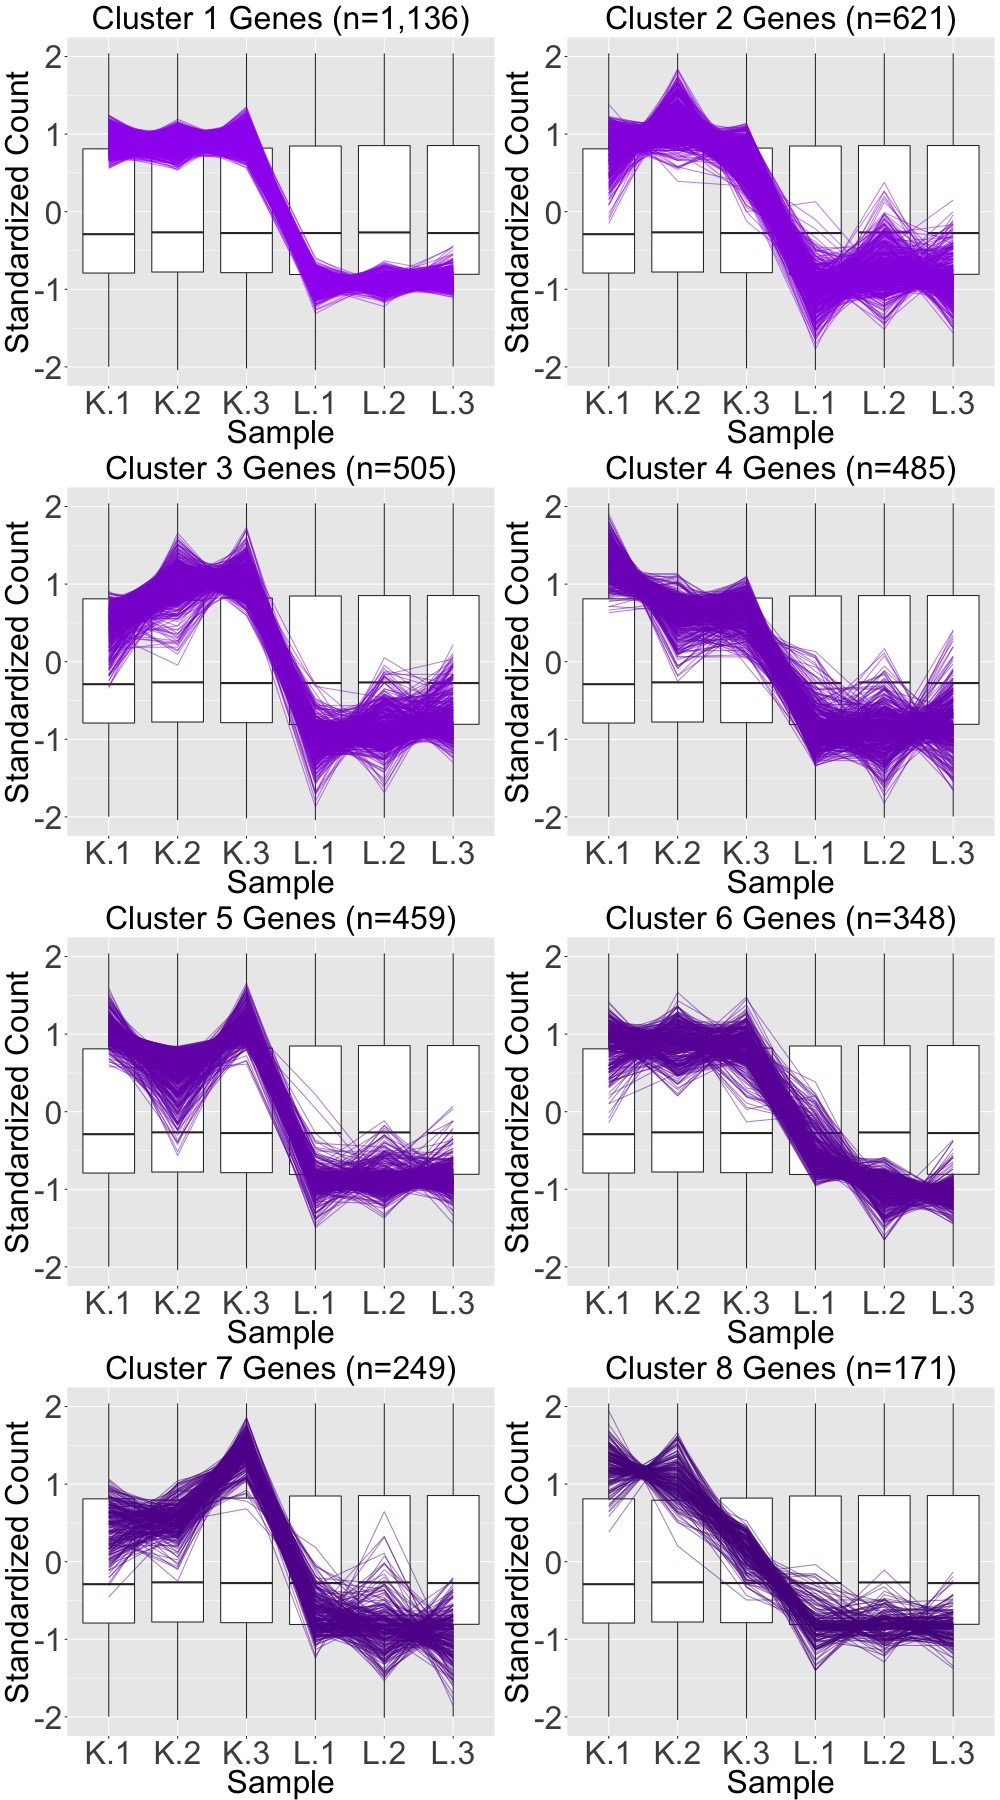
\includegraphics[width=0.65\columnwidth]{MakeFigures/lkClustersKeep.jpg}}
\end{framed}
\caption{Parallel coordinate plots showing eight hiearchical clusters from the 3,974 genes that remained in the kidney-specific DEGs after TMM normalization. We see that, for the most part, the parallel coordinate patterns follow the expected patterns across the clusters. The ideal pattern of DEGs is especially captured in the first cluster (the largest one with 1,136 genes). We applied ombre coloring across the clusters in order of cluster size. We used hierarchical clustering to tease apart subtle pattern differences and to mitigate additional overplotting that would occur if we were to plot all genes onto only one parallel coordinate plot.
\label{lkClustersKeep}}
\end{figure}

\null
\begin{figure}[t!]
\begin{framed}
\centerline{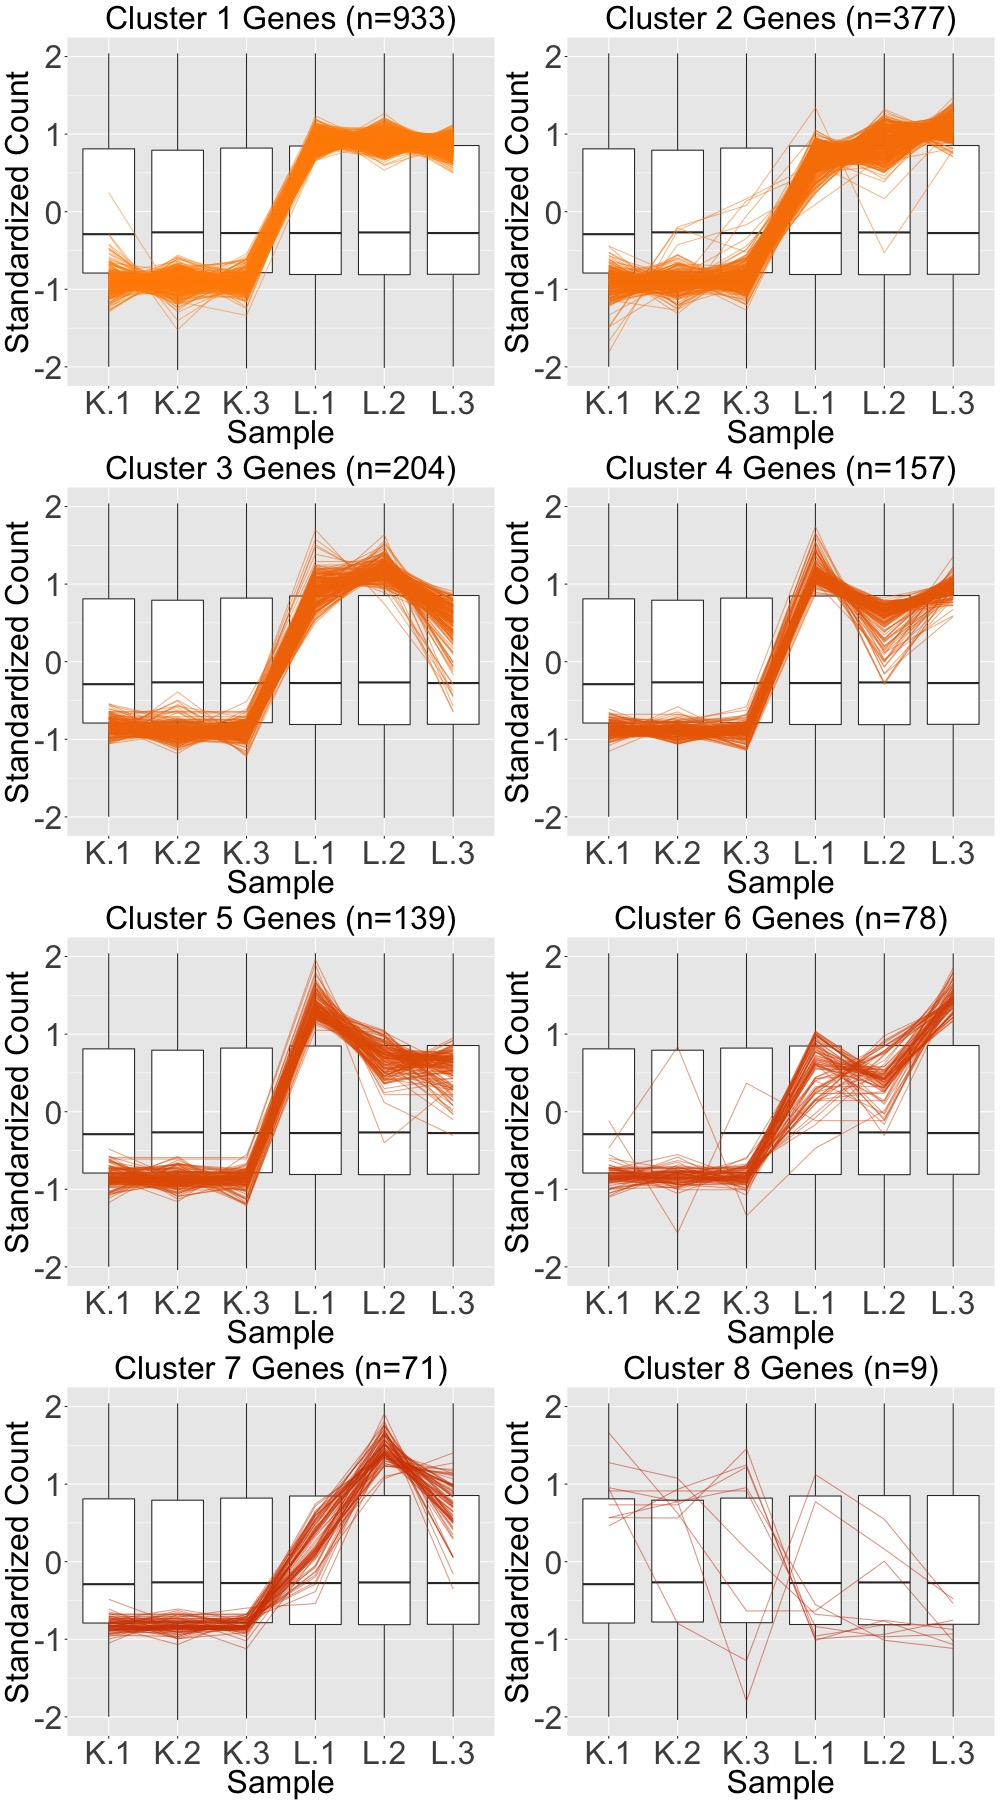
\includegraphics[width=0.65\columnwidth]{MakeFigures/lkClustersOrig.jpg}}
\end{framed}
\caption{Parallel coordinate plots showing eight hiearchical clusters from the 1,968 genes that remained in the liver-specific DEGs after TMM normalization. We see that, for the most part, the parallel coordinate patterns follow the expected patterns across the clusters. The ideal pattern of DEGs is especially captured in the first cluster (the largest one with 933 genes). We applied ombre coloring across the clusters in order of cluster size. We used hierarchical clustering to tease apart subtle pattern differences and to mitigate additional overplotting that would occur if we were to plot all genes onto only one parallel coordinate plot.
\label{lkClustersOrig}}
\end{figure}

\null
\begin{figure}[t!]
\begin{framed}
\centerline{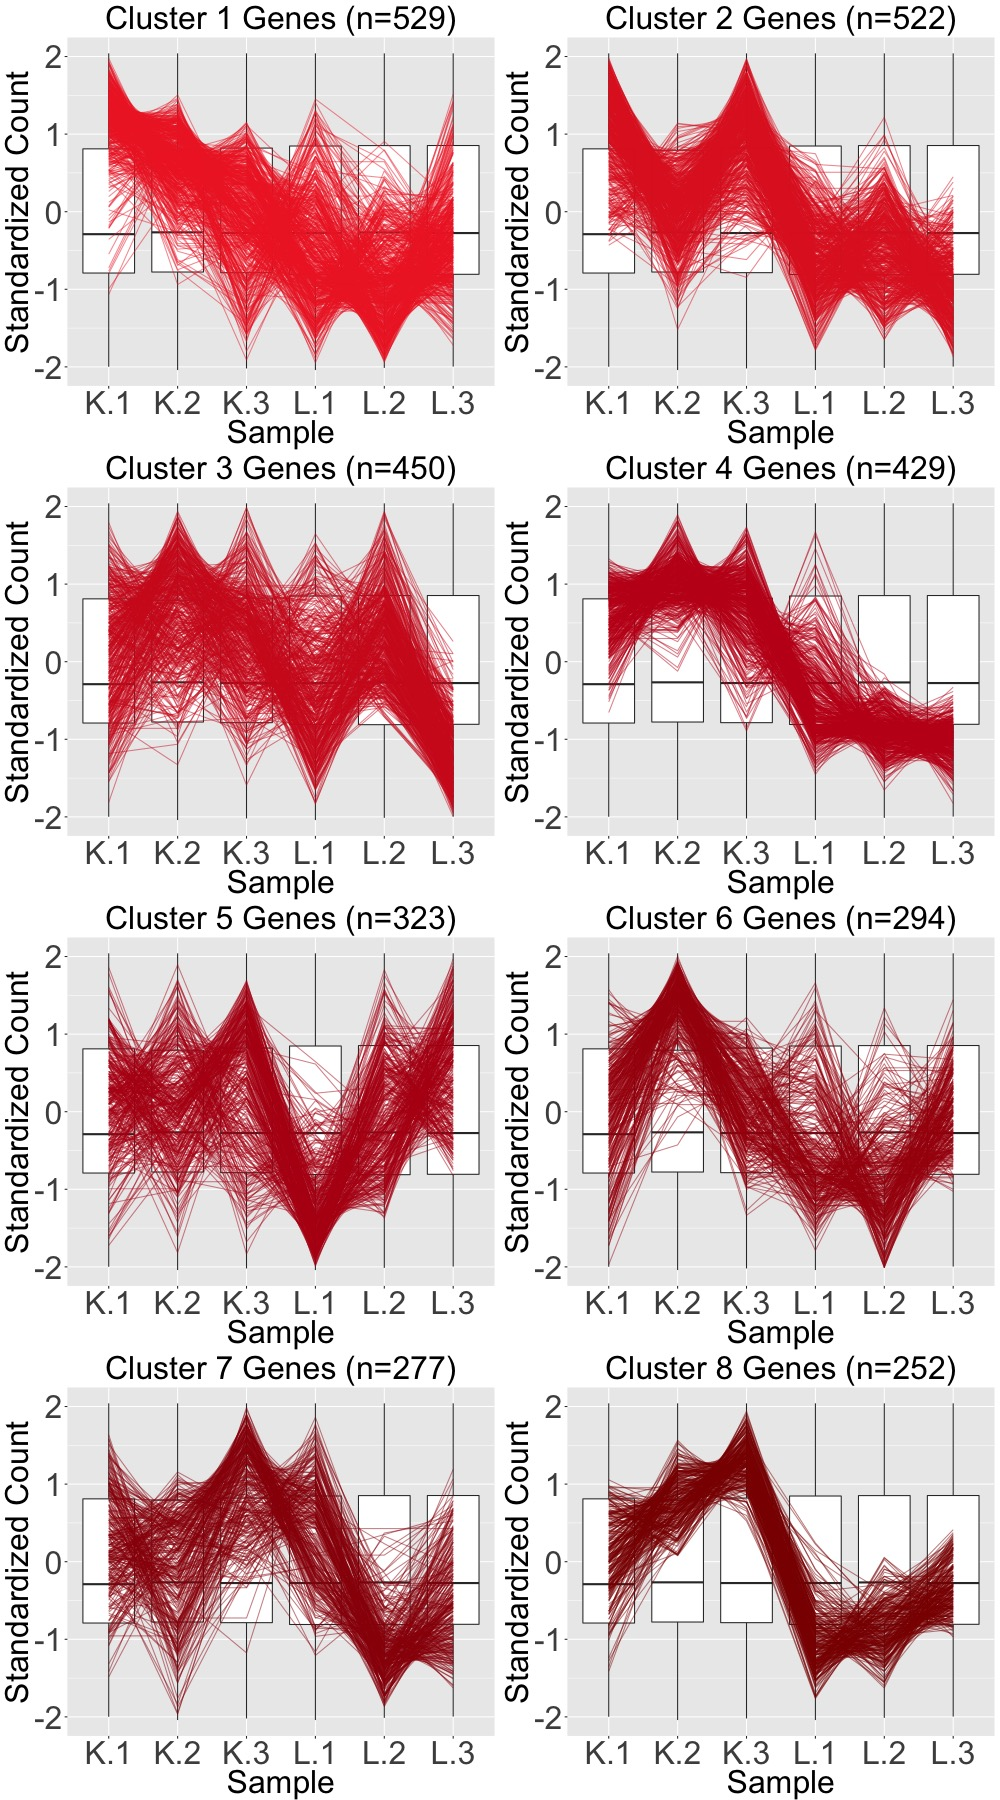
\includegraphics[width=0.65\columnwidth]{MakeFigures/lkClustersRemove.jpg}}
\end{framed}
\caption{Parallel coordinate plots showing eight hiearchical clusters from the 3,076 genes that were removed from the kidney-specific DEGs after TMM normalization. The patterns in almost all clusters do not resemble the expected DEG format; instead, they show large variability between replicates and small variability between treatments. In some clusters, it is difficult to even determine which group would be the overexpressed one if its genes were in fact DEGs. Taken together, this plot provides additional statistical evidence that the application of TMM normalization successfully removed genes that were previously mislabeled as kidney-specific DEGs with library scaling normalization. We applied ombre coloring across the clusters in order of cluster size. We used hierarchical clustering to tease apart subtle pattern differences and to mitigate additional overplotting that would occur if we were to plot all genes onto only one parallel coordinate plot.
\label{lkClustersRemove}}
\end{figure}

\null
\begin{figure}[t!]
\begin{framed}
\centerline{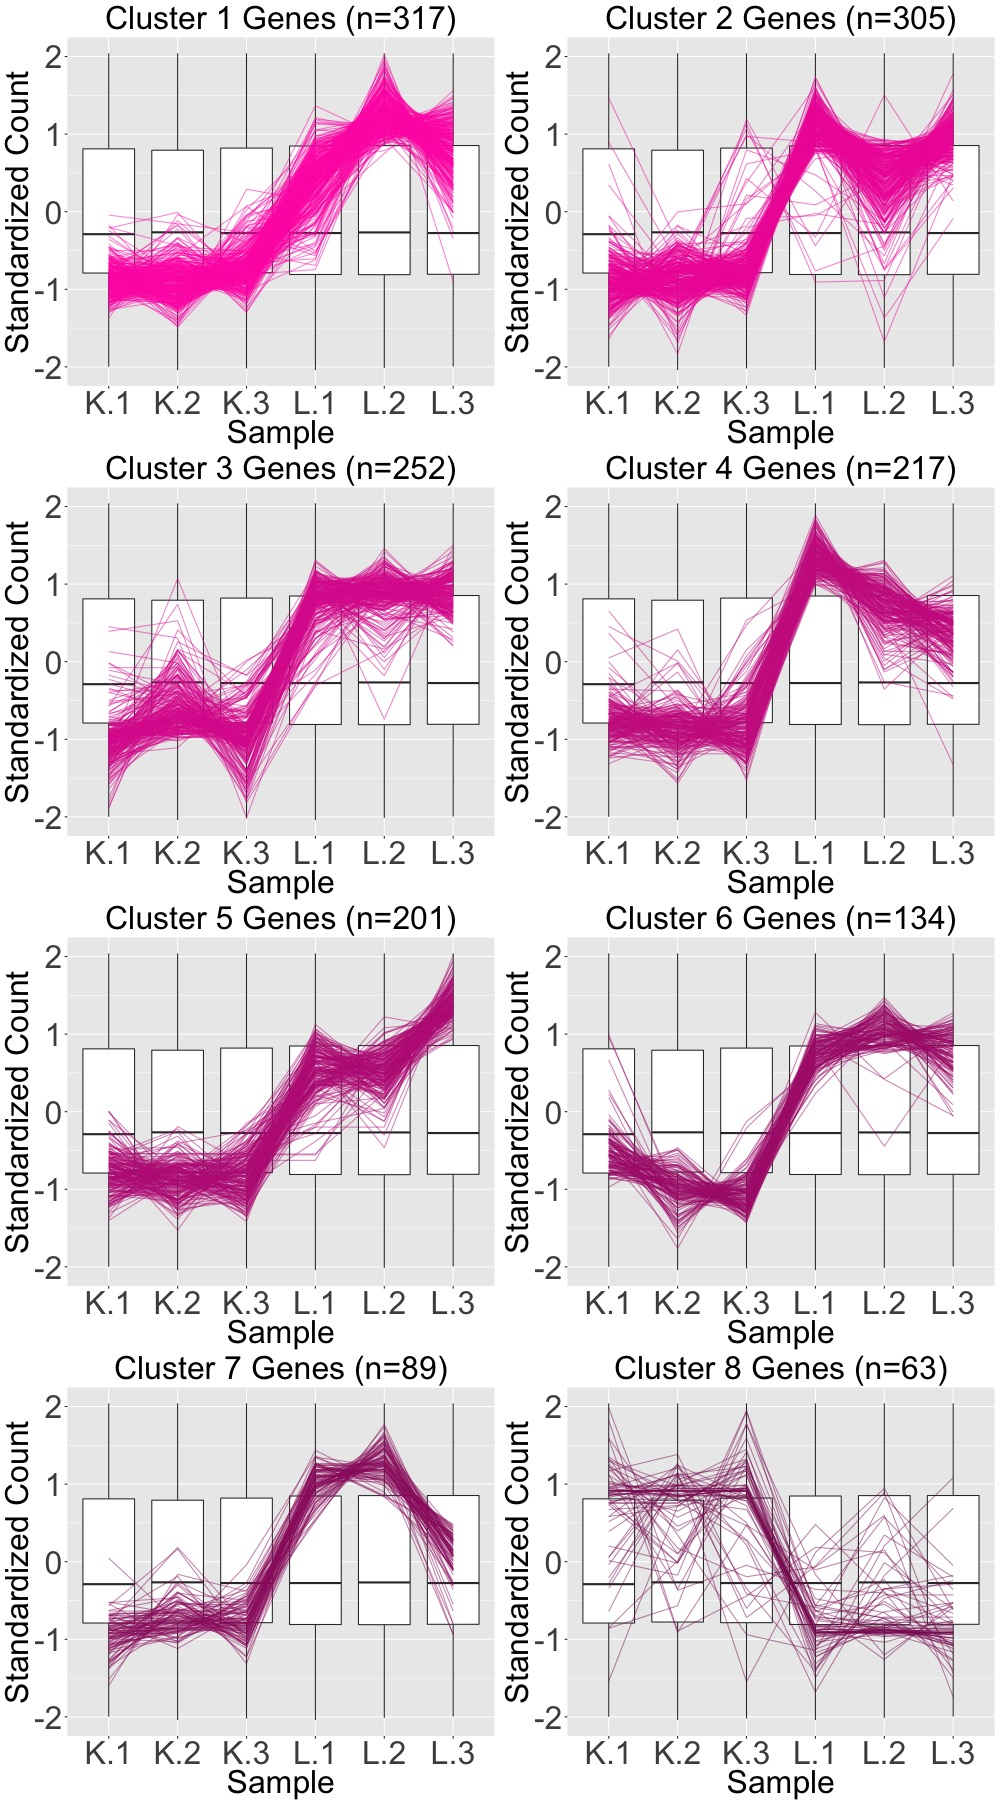
\includegraphics[width=0.65\columnwidth]{MakeFigures/lkClustersAdd.jpg}}
\end{framed}
\caption{Parallel coordinate plots showing eight hiearchical clusters from the 1,578 genes that were \textit{added} as liver-specific DEGs after TMM normalization. We see that, for the most part, the parallel coordinate lines follow the expected patterns across the clusters, but not as precisely as we saw with the purple (Figure~\ref{lkClustersKeep}) and orange (Figure~\ref{lkClustersOrig}) gene subsets. We applied ombre coloring across the clusters in order of cluster size. We used hierarchical clustering to tease apart subtle pattern differences and to mitigate additional overplotting that would occur if we were to plot all genes onto only one parallel coordinate plot.
\label{lkClustersAdd}}
\end{figure}

\null
\begin{figure}[t!]
\begin{framed}
\centerline{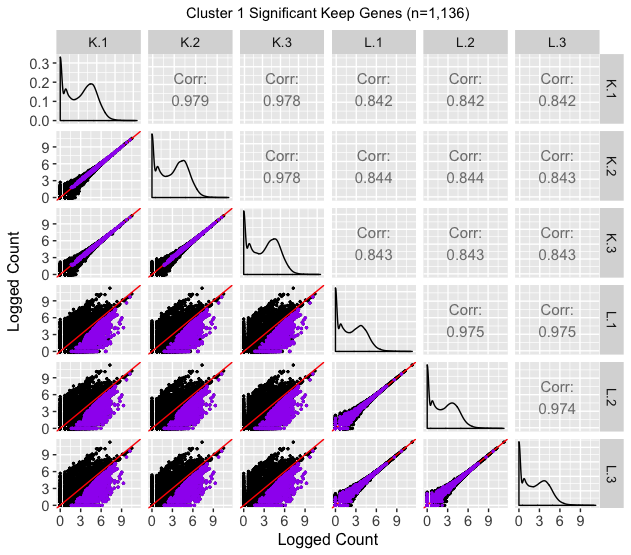
\includegraphics[width=1\columnwidth]{MakeFigures/lkClustersKeepSM.jpg}}
\end{framed}
\caption{Scatterplot matrix of the 1,136 genes that were in the first cluster (of Figure~\ref{lkClustersKeep}) from genes that remained as kidney-specific DEGs even after TMM normalization. With this scatterplot matrix, we verify from an additional perspective that these genes demonstrate the expected patterns of DEGs.
\label{lkClustersKeepSM}}
\end{figure}

\null
\begin{figure}[t!]
\begin{framed}
\centerline{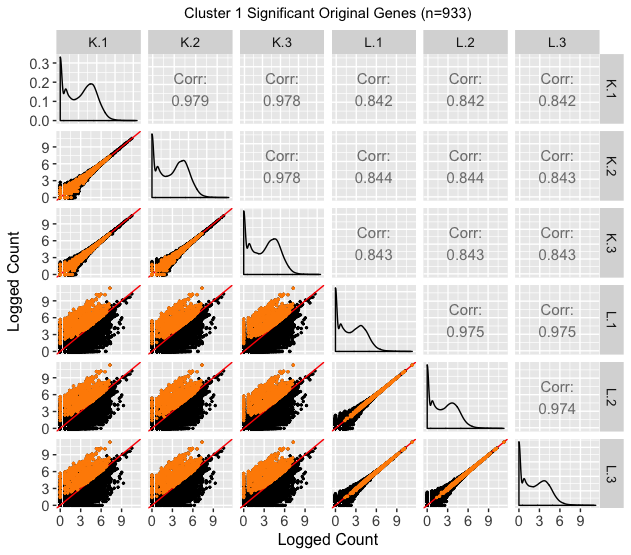
\includegraphics[width=1\columnwidth]{MakeFigures/lkClustersOrigSM.jpg}}
\end{framed}
\caption{Scatterplot matrix of the 933 genes that were in the first cluster (of Figure~\ref{lkClustersOrig}) from genes that remained as liver-specific DEGs even after TMM normalization. With this scatterplot matrix, we verify from an additional perspective that these genes demonstrate the expected patterns of DEGs.
\label{lkClustersOrigSM}}
\end{figure}

\null
\begin{figure}[t!]
\begin{framed}
\centerline{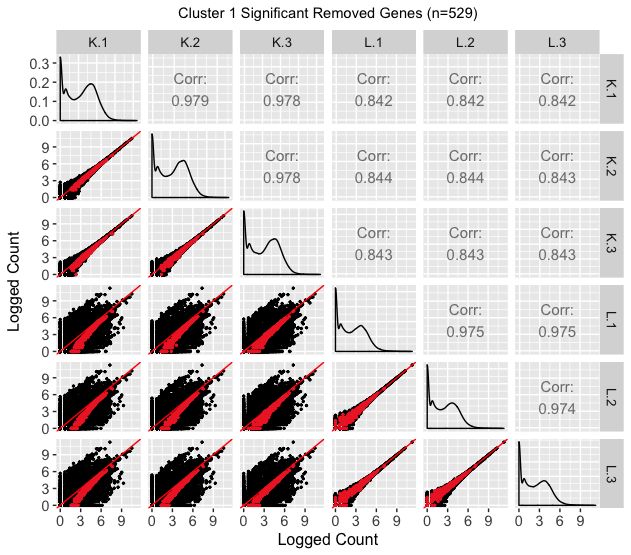
\includegraphics[width=1\columnwidth]{MakeFigures/lkClustersRemoveSM.jpg}}
\end{framed}
\caption{Scatterplot matrix of the 529 genes that were in the first cluster (of Figure~\ref{lkClustersRemove}) from genes that no longer remained as kidney-specific DEGs after TMM normalization. With this scatterplot matrix, we verify from an additional perspective that these genes do \textit{not} demonstrate the expected patterns of DEGs too strongly (they do not deviate much from the \textit{x=y} line in the treatment scatterplots). This provides additional evidence that TMM normalization removing these genes from DEG status may be valid.
\label{lkClustersRemoveSM}}
\end{figure}

\null
\begin{figure}[t!]
\begin{framed}
\centerline{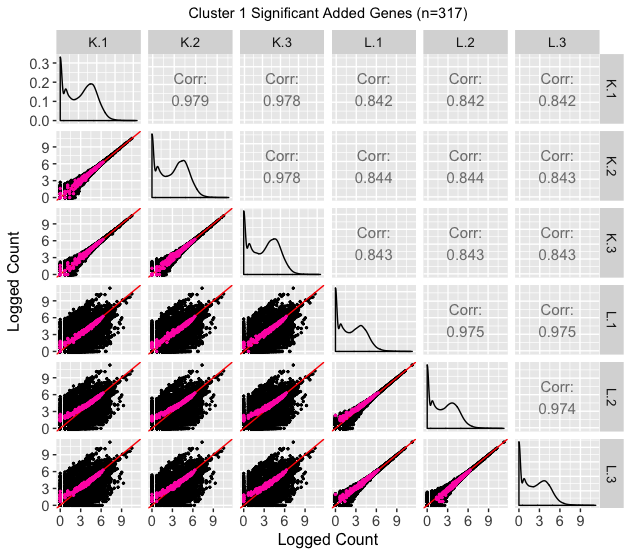
\includegraphics[width=1\columnwidth]{MakeFigures/lkClustersAddSM.jpg}}
\end{framed}
\caption{Scatterplot matrix of the 317 genes that were in the first cluster (of Figure~\ref{lkClustersAdd}) from genes that were \textit{added} as liver-specific DEGs after TMM normalization. With this scatterplot matrix, we see that the genes do \textit{not} demonstrate the expected patterns of DEGs too strongly (they do not deviate much from the \textit{x=y} line in the treatment scatterplots). In fact, these pink genes appear similarly to what we saw from the scatterplot matrix of the red genes (Figure~\ref{lkClustersRemoveSM}). This is somewhat of a surprise, given that the pink genes were \textit{added} by TMM  normalization, while the red genes were \textit{removed} by TMM normalization. Stated differently, we would expect the pink genes to appear more like differentially expressed genes if TMM normalization is appropriate, but we could not confirm this expectation. We will return to this problem later in the supplementary file.
\label{lkClustersAddSM}}
\end{figure}


\null
\begin{figure}[t!]
\begin{framed}
\centerline{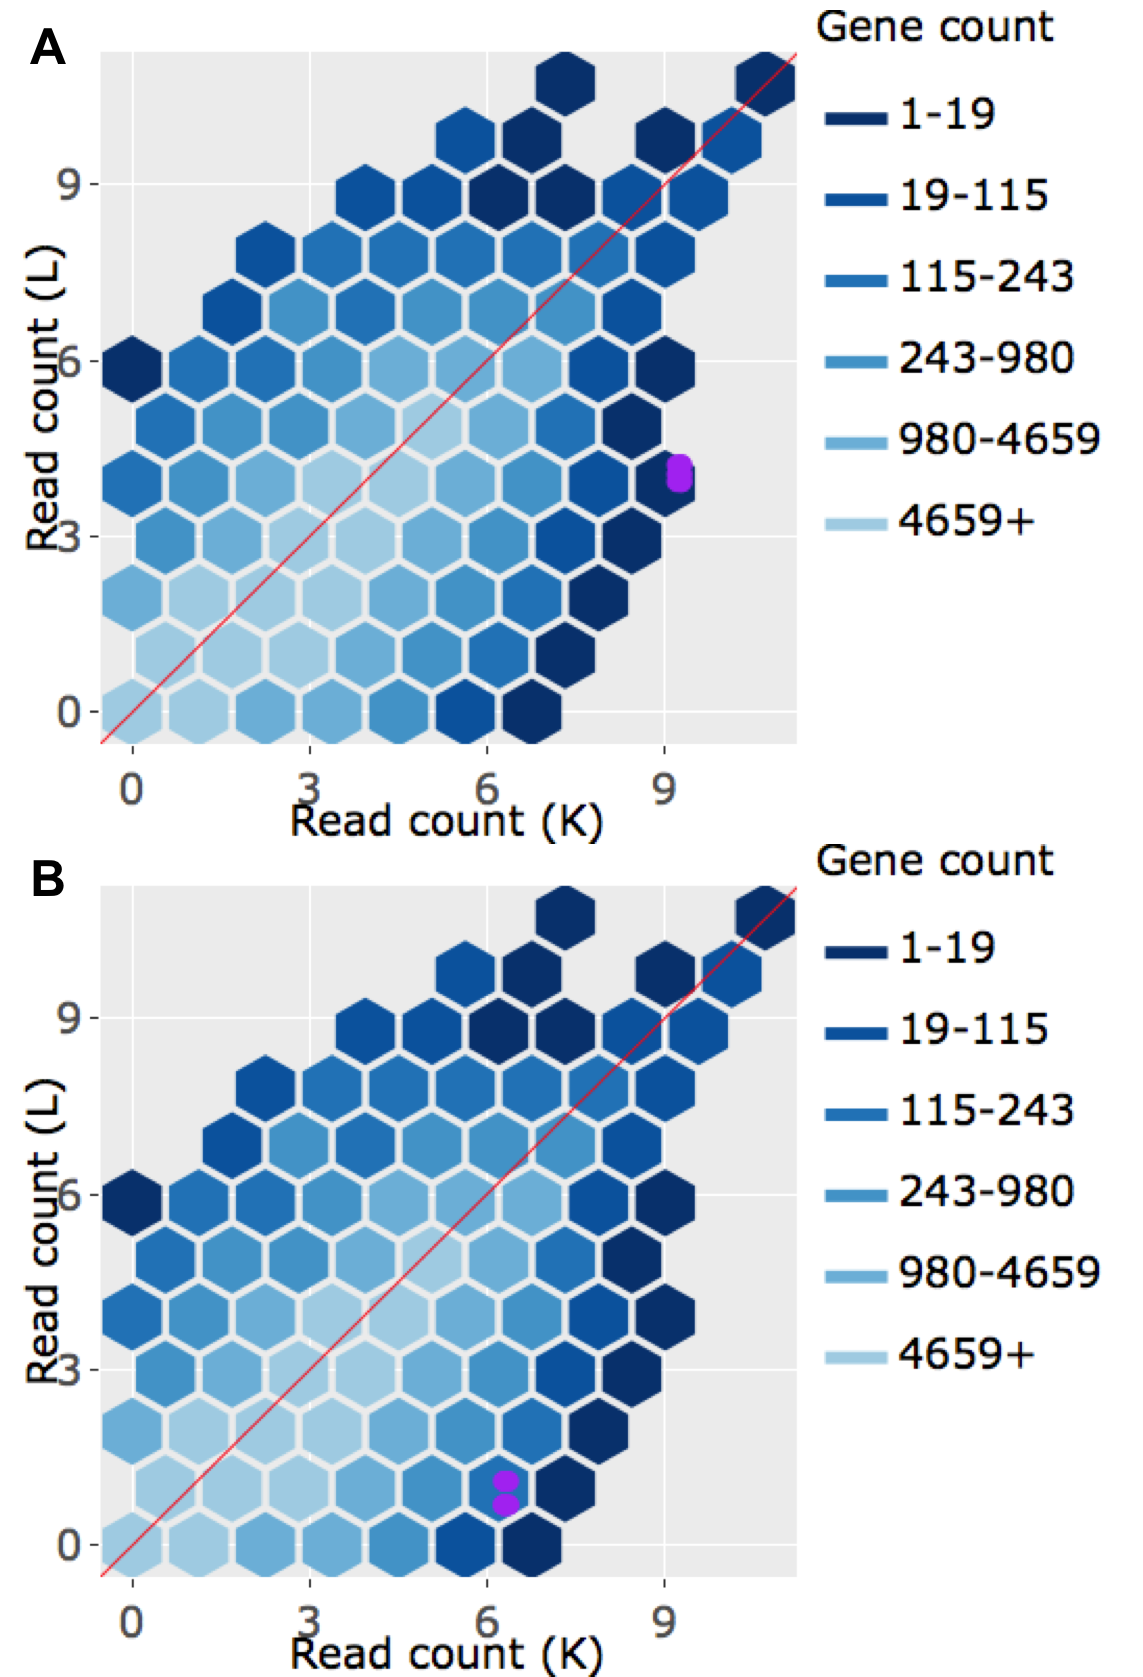
\includegraphics[width=0.7\columnwidth]{MakeFigures/Dashboards/litreClusterKeep/litreClusterKeep.jpg}}
\end{framed}
\caption{Example litre plots from the 1,136 genes that were in the first cluster (Figure~\ref{lkClustersKeep}) of genes that remained as kidney-specific DEGs even after TMM normalization. With these litre plots, we verify from an additional perspective that these genes demonstrate the expected patterns of DEGs.
\label{litreClusterKeep}}
\end{figure}

\null
\begin{figure}[t!]
\begin{framed}
\centerline{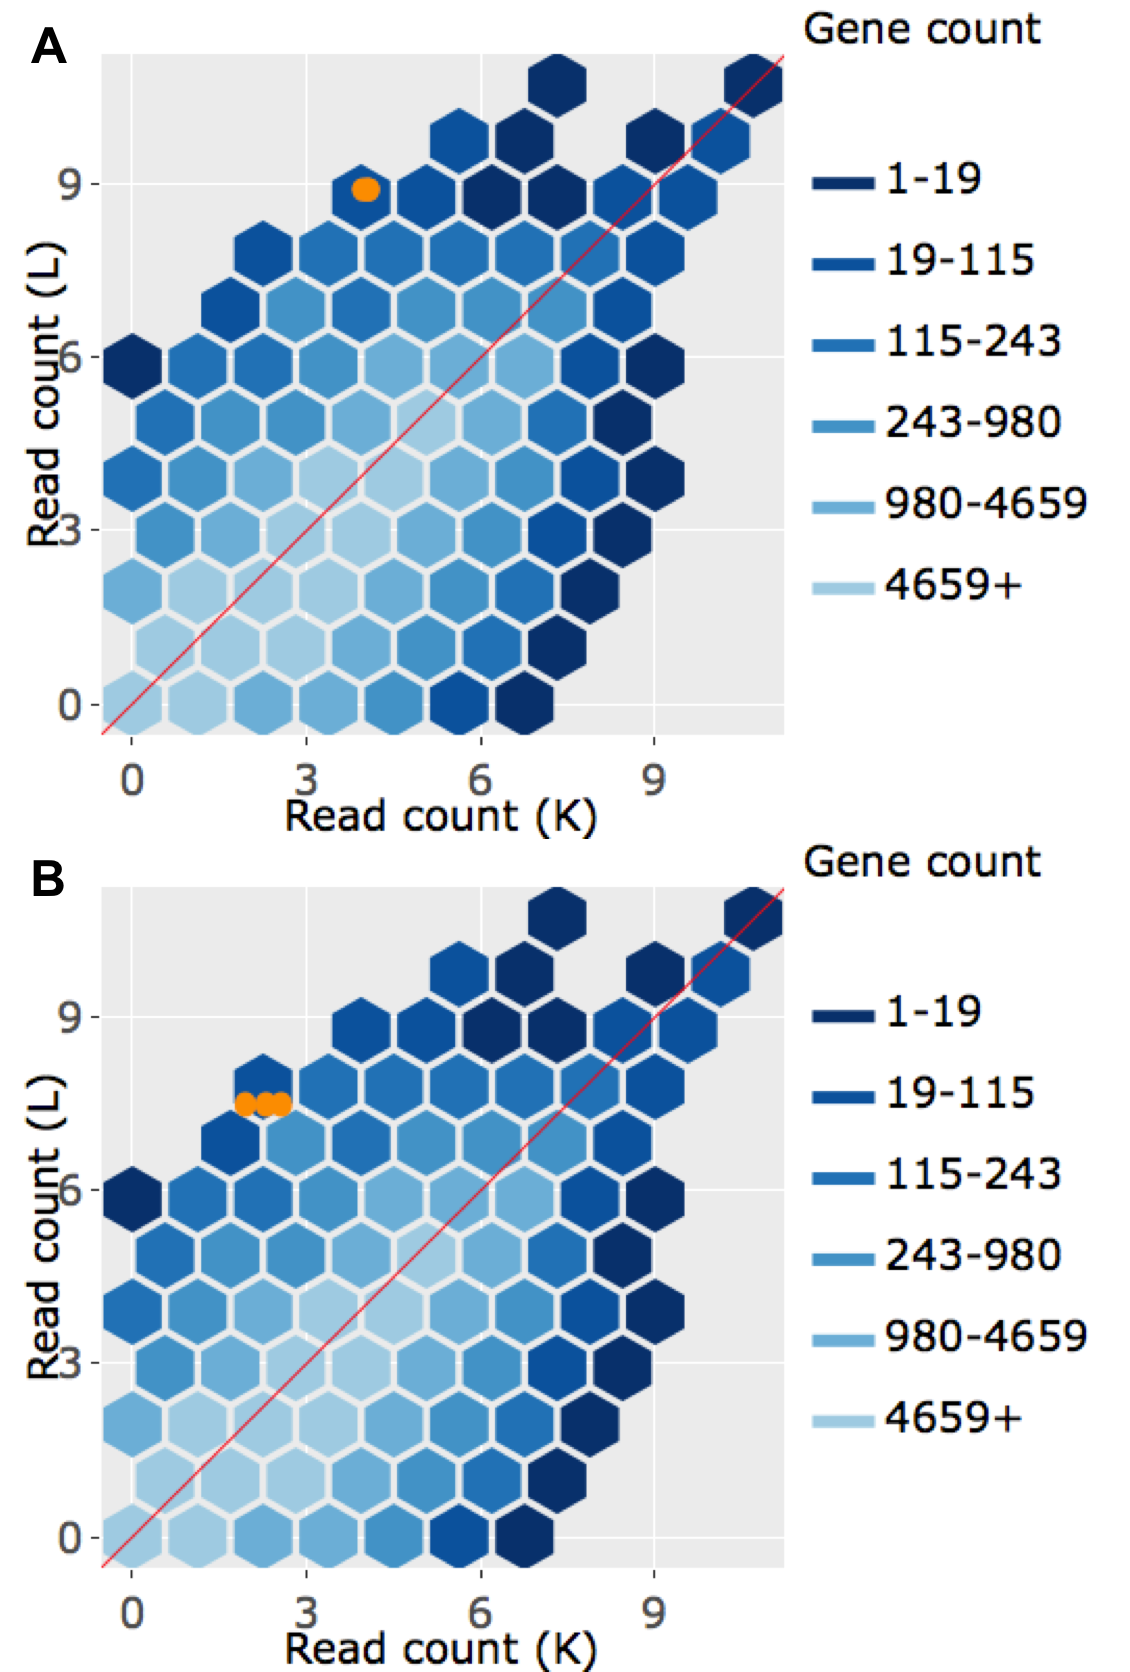
\includegraphics[width=0.7\columnwidth]{MakeFigures/Dashboards/litreClusterOrig/litreClusterOrig.jpg}}
\end{framed}
\caption{Example litre plots from the 933 genes that were in the first cluster (Figure~\ref{lkClustersOrig}) from genes that remained as liver-specific DEGs even after TMM normalization. With these litre plots, we verify from an additional perspective that these genes demonstrate the expected patterns of DEGs.
\label{litreClusterOrig}}
\end{figure}

\null
\begin{figure}[t!]
\begin{framed}
\centerline{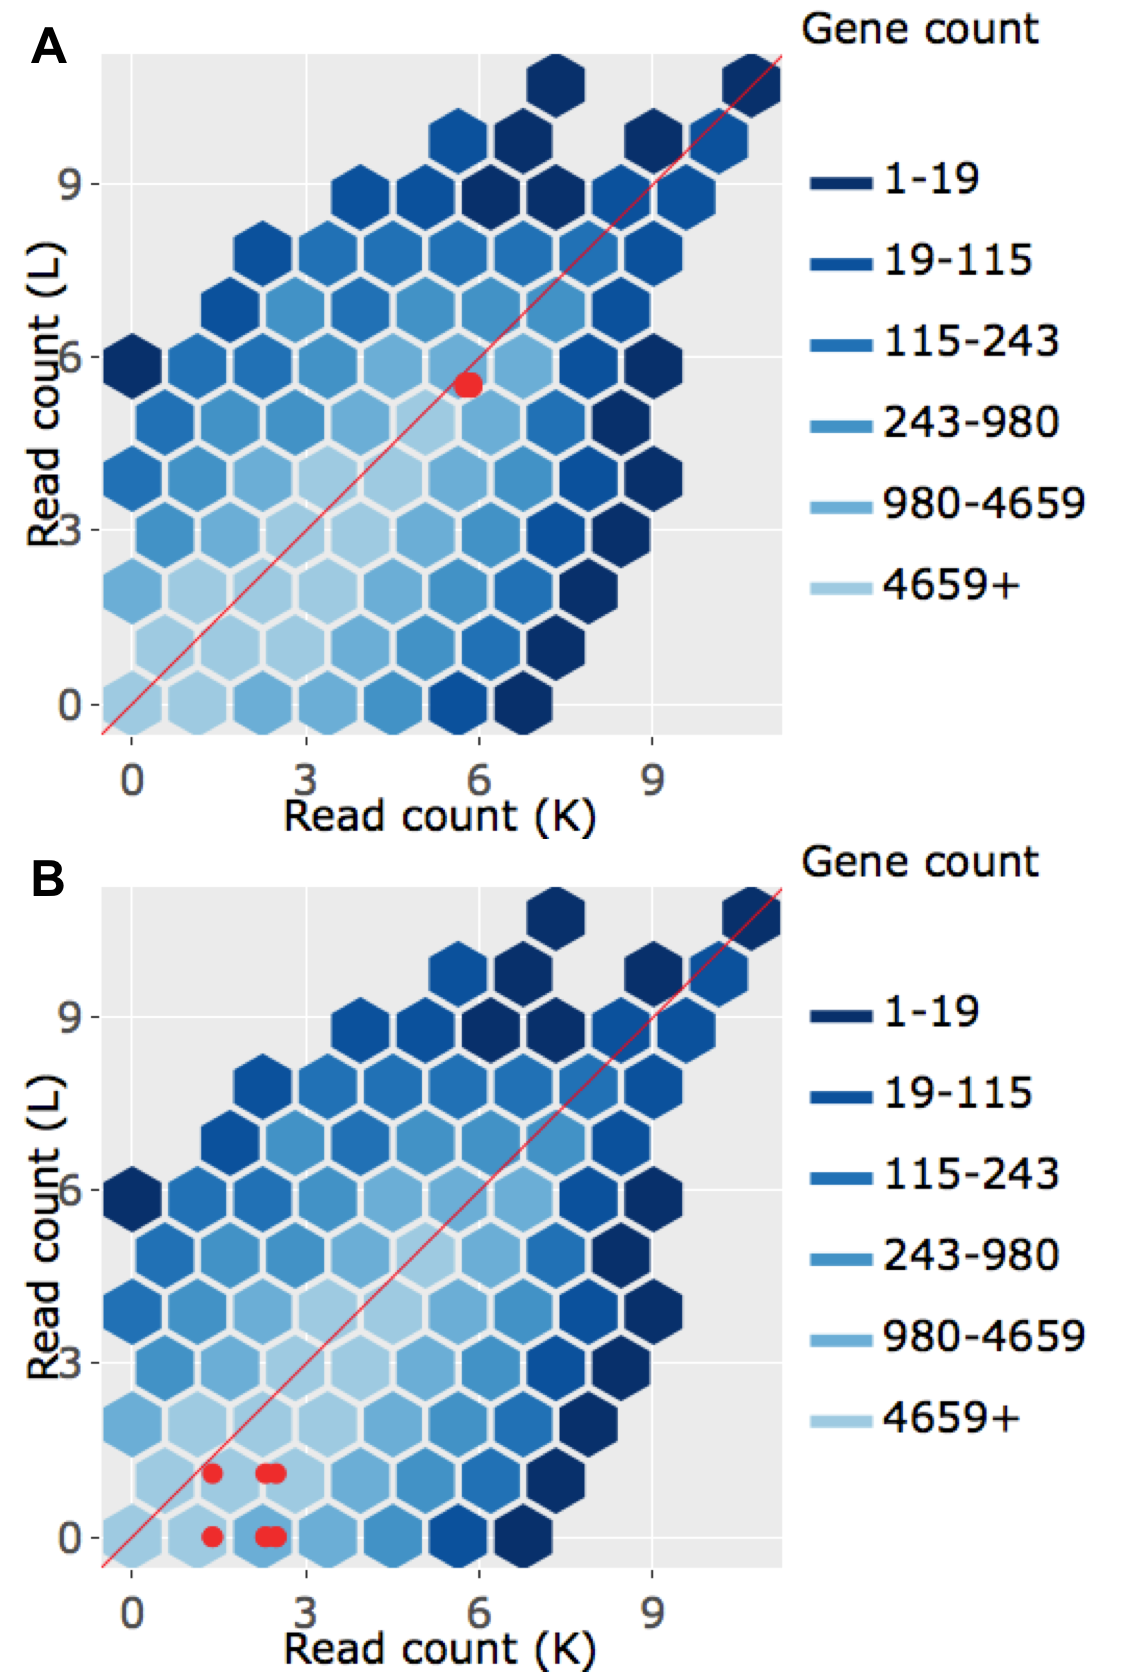
\includegraphics[width=0.7\columnwidth]{MakeFigures/Dashboards/litreClusterRemove/litreClusterRemove.jpg}}
\end{framed}
\caption{Example litre plots from the 529 genes that were in the first cluster (Figure~\ref{lkClustersRemove}) of genes that no longer remained as kidney-specific DEGs after TMM normalization. With these litre plots, we verify from an additional perspective that these genes do not demonstrate the expected patterns of DEGs. This provides additional evidence that TMM normalization removing these genes from DEG status may be valid.
\label{litreClusterRemove}}
\end{figure}

\null
\begin{figure}[t!]
\begin{framed}
\centerline{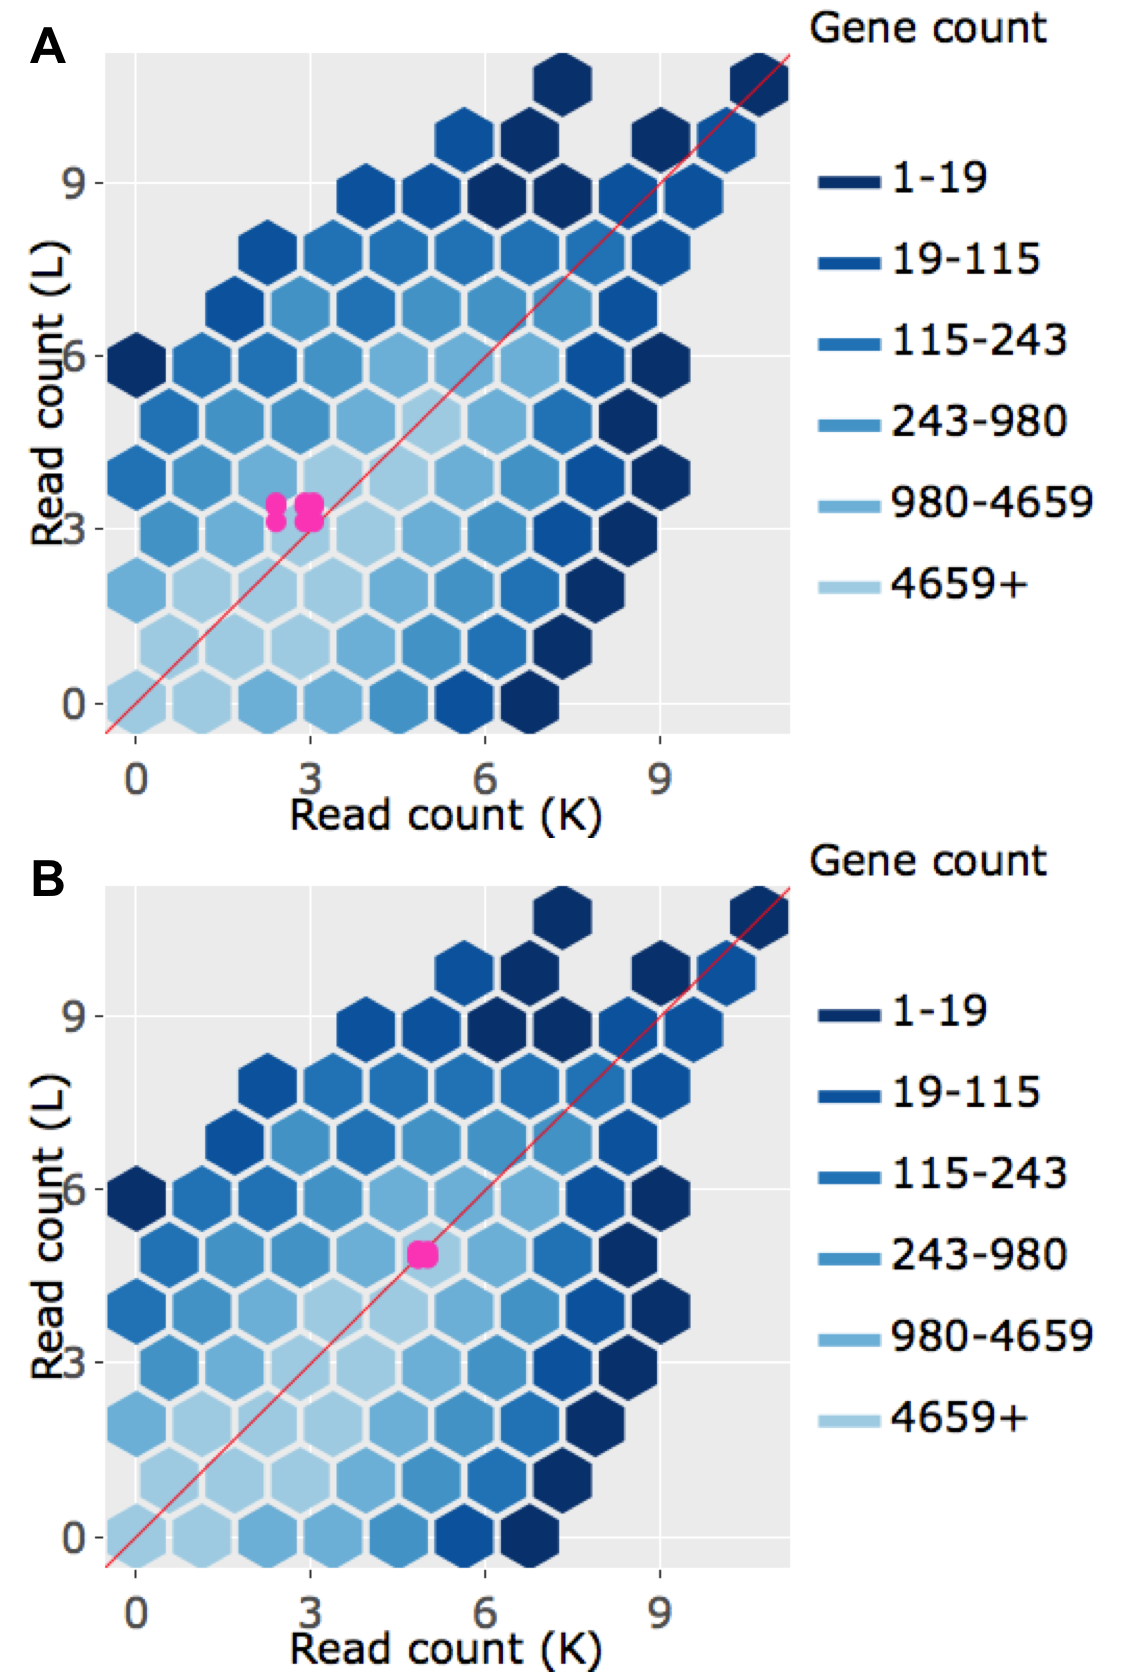
\includegraphics[width=0.7\columnwidth]{MakeFigures/Dashboards/litreClusterAdd/litreClusterAdd.jpg}}
\end{framed}
\caption{Example litre plots from the 317 genes that were in the first cluster (Figure~\ref{lkClustersAdd}) from genes that were \textit{added} as liver-specific DEGs after TMM normalization. With these litre plots, we see that the genes do \textit{not} demonstrate the expected patterns of DEGs in a trustworthy manner. In fact, these pink genes appear similarly to what we saw from the example litre plots of the red genes (Figure~\ref{litreClusterRemove}). This is somewhat of a surprise, given that the pink genes were \textit{added} by TMM  normalization, while the red genes were \textit{removed} by TMM normalization. Stated differently, we would expect the pink genes to appear more like differentially expressed genes if TMM normalization is appropriate, but we could not confirm this expectation. We will return to this problem later in the supplementary file.
\label{litreClusterAdd}}
\end{figure}

\null
\begin{figure}[t!]
\begin{framed}
\centerline{\includegraphics[width=1\columnwidth]{MakeFigures/lkClustersKeepSM-St.jpg}}
\end{framed}
\caption{Scatterplot matrix of the \textit{standardized} 1,136 genes that were in the first cluster (Figure~\ref{lkClustersKeep}) from genes that remained as kidney-specific DEGs even after TMM normalization. Even though the standardization process removes the interesting geometrical features we saw back in Figure~\ref{lkClustersKeepSM} regarding the streak of overexpressed liver genes, it amplifies other patterns in meaningful ways. For instance, compared to Figure~\ref{lkClustersKeepSM}, the highlighted genes here appear more clustered and separated from the \textit{x=y} line in the treatment scatterplots, and more clustered and connected to the \textit{x=y} line in the replicate scatterplots. We can also now see more clearly in the replicate scatterplots that the kidney expression is higher than the liver expression.
\label{lkClustersKeepSM-St}}
\end{figure}

\null
\begin{figure}[t!]
\begin{framed}
\centerline{\includegraphics[width=1\columnwidth]{MakeFigures/lkClustersOrigSM-St.jpg}}
\end{framed}
\caption{Scatterplot matrix of the \textit{standardized} 933 genes that were in the first cluster (Figure~\ref{lkClustersOrig}) from genes that remained as liver-specific DEGs even after TMM normalization. Even though the standardization process removes the interesting geometrical features we saw back in Figure~\ref{lkClustersOrigSM} regarding the streak of overexpressed liver genes, it amplifies other patterns in meaningful ways. For instance, compared to Figure~\ref{lkClustersOrigSM}, the highlighted genes here appear more clustered and separated from the \textit{x=y} line in the treatment scatterplots, and more clustered and connected to the \textit{x=y} line in the replicate scatterplots. We can also now see more clearly in the replicate scatterplots that the liver expression is higher than the kidney expression. 
\label{lkClustersOrigSM-St}}
\end{figure}

\null
\begin{figure}[t!]
\begin{framed}
\centerline{\includegraphics[width=1\columnwidth]{MakeFigures/lkClustersRemoveSM-St.jpg}}
\end{framed}
\caption{Scatterplot matrix of the \textit{standardized} 529 genes that were in the first cluster (Figure~\ref{lkClustersRemove}) from genes that no longer remained as kidney-specific DEGs after TMM normalization. Even though the standardization process removes the interesting geometrical features we saw back in Figure~\ref{lkClustersRemoveSM} regarding the streak of overexpressed liver genes, it allows us to view the DEG patterns in a different meaningful fashion. Namely, the genes of interest are now spread out more, and the replicate and treatment scatterplots are almost indistinguishable from each other, with both of them showing genes of interest crossing both sides of the \textit{x=y} line. In other words, standardization of the data provides additional visualization evidence that TMM normalization was justified in removing these genes from DEG designation. 
\label{lkClustersRemoveSM-St}}
\end{figure}

\null
\begin{figure}[t!]
\begin{framed}
\centerline{\includegraphics[width=1\columnwidth]{MakeFigures/lkClustersAddSM-St.jpg}}
\end{framed}
\caption{Scatterplot matrix of the \textit{standardized} 317 genes that were in the first cluster (Figure~\ref{lkClustersAdd}) from genes that were \textit{added} as liver-specific DEGs after TMM normalization. Even though the standardization process removes the interesting geometrical features we saw back in Figure~\ref{lkClustersAddSM} regarding the streak of overexpressed liver genes, it allows us to view the DEG patterns in a different meaningful fashion. Namely, the genes of interest are now spread out more, and we can now distinguish the replicate and treatment scatterplots more clearly. For the most part, the genes of interest deviate from the \textit{x=y} line in the treatment scatterplots more so than in the replicate scatterplots, and hence display somewhat of the pattern of differential expression. In fact, the pink genes again appear as an intermediate between the purple and orange genes that clearly display differential expression (Figures~\ref{lkClustersKeepSM-St} and~\ref{lkClustersOrigSM-St}) and the red genes that clearly do \textit{not} display differential expression (Figure~\ref{lkClustersRemoveSM-St}). In other words, standardized scatterplot matrices provide additional visualization evidence that TMM normalization was justified in removing the red genes from and adding the pink genes to DEG designation.
\label{lkClustersAddSM-St}}
\end{figure}

\null
\begin{figure}[t!]
\begin{framed}
\centerline{\includegraphics[width=0.7\columnwidth]{MakeFigures/Dashboards/litreClusterKeep-St/litreClusterKeep-St.jpg}}
\end{framed}
\caption{Example \textit{standardized} litre plots from the 1,136 genes that were in the first cluster (Figure~\ref{lkClustersKeep}) of genes that remained as kidney-specific DEGs even after TMM normalization. With standardization, we immediately note that the original geometric structure that elicited meaningful information about variation between treatments and replicates as well as the problematic streak of over-expressed liver genes is now gone. However, we confirm that these standardized litre plots corroborate the corresponding non-standardized litre plots we saw in Figure~\ref{litreClusterKeep} that these purple genes demonstrate the expected patterns of DEGs.
\label{litreClusterKeep-St}}
\end{figure}

\null
\begin{figure}[t!]
\begin{framed}
\centerline{\includegraphics[width=0.7\columnwidth]{MakeFigures/Dashboards/litreClusterOrig-St/litreClusterOrig-St.jpg}}
\end{framed}
\caption{Example litre plots from the 933 genes that were in the first cluster (Figure~\ref{lkClustersOrig}) from genes that remained as liver-specific DEGs even after TMM normalization. With standardization, we immediately note that the original geometric structure that elicited meaningful information about variation between treatments and replicates as well as the problematic streak of over-expressed liver genes is now gone. However, we confirm that these standardized litre plots corroborate the corresponding non-standardized litre plots we saw in Figure~\ref{litreClusterOrig} that these orange genes demonstrate the expected patterns of DEGs.
\label{litreClusterOrig-St}}
\end{figure}

\null
\begin{figure}[t!]
\begin{framed}
\centerline{\includegraphics[width=\columnwidth]{MakeFigures/Dashboards/litreClusterRemove-St/litreClusterRemove-St.jpg}}
\end{framed}
\caption{\textit{Standardized} litre plots for the nine genes with the lowest FDR values out of the 529 genes that were in the first cluster (Figure~\ref{lkClustersRemove}) of genes that no longer remained as kidney-specific DEGs after TMM normalization. As with the corresponding non-standardized litre plots in Figure~\ref{litreClusterRemove}, we verify from an additional perspective that the red genes do not demonstrate the expected patterns of DEGs. The example red genes here are show much larger inconsistencies between replicates than what we saw with the purple (Figure~\ref{litreClusterKeep-St}) and orange (Figure~\ref{litreClusterOrig-St}) genes. This provides additional evidence that TMM normalization removing these genes from DEG status may be valid.
\label{litreClusterRemove-St}}
\end{figure}

\null
\begin{figure}[t!]
\begin{framed}
\centerline{\includegraphics[width=\columnwidth]{MakeFigures/Dashboards/litreClusterAdd-St/litreClusterAdd-St.jpg}}
\end{framed}
\caption{\textit{Standardized} litre plots for the nine genes with the lowest FDR values out of the 317 genes that were in the first cluster (Figure~\ref{lkClustersAdd}) from genes that were \textit{added} as liver-specific DEGs after TMM normalization. While non-standardized litre plots showed similar profiles between the red (Figure~\ref{litreClusterRemove}) and pink (Figure~\ref{litreClusterAdd}) genes, standardization amplifies the differences in a manner we would expect. Namely, we can now quickly determine that the pink profiles in this figure show patterns more akin to differential expression than the red profiles in Figure~\ref{litreClusterRemove-St}. That is, the overlaid pink points deviate more from the \textit{x=y} line in a tight cluster than the overlaid red points. At the same time, the overlaid pink points here show patterns less akin to differential expression than the purple (Figure~\ref{litreClusterKeep-St}) and orange (Figure~\ref{litreClusterOrig-St}) points. All together, the standardized litre plots place the pink gene profiles as an intermediate between the clean-looking purple and orange genes and the messy-looking red genes, which is to be expected if TMM normalization is the more appropriate technique.
\label{litreClusterAdd-St}}
\end{figure}



%%%%%%%%%%%%%%%%%%%%%%%%%%%%%%%%%%%%%%%%%%%%%%%%%%%%%%%%%%%%%%%%
%%%%%%%%%%%%%%%%%%%%%%%%%%%%%%%%%%%%%%%%%%%%%%%%%%%%%%%%%%%%%%%%

\chapter{Supplementary material for Chapter 4}
\label{sec:suppchapter3}

This section contains additional example video demonstrations of the interactive visualization methods from our work-in-progress \pkg{R} package \pkg{bigPint}. It also includes the software reference manual for the software package.

\begin{figure}[H]
    \begin{framed}
    \centering
    \includemedia[width=1.0\textwidth, addresource=scatMatOrth.mov, deactivate=onclick, flashvars={source=scatMatOrth.mov}]{\includegraphics{./scatMatOrth.jpg}}{VPlayer.swf}
    \end{framed}
    \caption{This video demonstrates an interactive scatterplot matrix that allows users to threshold based on orthogonal distance from the \text{x=y} line. Upon clicking on this figure twice, a short video demonstrating the animation features for this function can be viewed. Please note that to properly view this video, the PDF version of this paper must be opened in Adobe Acrobat Reader DC (Version >=9), which can be downloaded free of charge.}
    \label{fig:scatMatOrth}
\end{figure}

\begin{figure}[H]
    \begin{framed}
    \centering
    \includemedia[width=1.0\textwidth, addresource=scatMatFC.mov, deactivate=onclick, flashvars={source=scatMatFC.mov}]{\includegraphics{./scatMatFC.jpg}}{VPlayer.swf}
    \end{framed}
    \caption{This video demonstrates an interactive scatterplot matrix that allows users to threshold based on fold change. Upon clicking on this figure twice, a short video demonstrating the animation features for this function can be viewed. Please note that to properly view this video, the PDF version of this paper must be opened in Adobe Acrobat Reader DC (Version >=9), which can be downloaded free of charge.}
    \label{fig:scatMatFC}
\end{figure}

\begin{figure}[H]
    \begin{framed}
    \centering
    \includemedia[width=1.0\textwidth, addresource=pcpPlotlyMarkers.mov, deactivate=onclick, flashvars={source=scatMatFC.mov}]{\includegraphics{./pcpPlotlyMarkers.jpg}}{VPlayer.swf}
    \end{framed}
    \caption{This video demonstrates an interactive parallel coordinate plot from the Plotly package. While it allows for the full capabilities in the Plotly Modebar (such as panning, zooming, and hovering), it does not allow the user to select lines unless the selection overlaps at an integer value on the x axis. It also does not allow users to print the names of any lines selected and possibly delete them. When working with a large number of parallel coordinate lines (say as genes), these interactive functionalities can be severaly limited. We improve upon this basic functionality in our software, as is demonstrated in the video of Figure~\ref{fig:pcpSeqSel}. Upon clicking on this figure twice, a short video demonstrating the animation features for this function can be viewed. Please note that to properly view this video, the PDF version of this paper must be opened in Adobe Acrobat Reader DC (Version >=9), which can be downloaded free of charge.}
    \label{fig:pcpPlotlyMarkers}
\end{figure}

\begin{figure}[H]
    \begin{framed}
    \centering
    \includemedia[width=1.0\textwidth, addresource=pcpSeqSel.mov, deactivate=onclick, flashvars={source=scatMatFC.mov}]{\includegraphics{./pcpSeqSel.jpg}}{VPlayer.swf}
    \end{framed}
    \caption{This video demonstrates improvements we made based upon basic functionality for parallel coordinate plots in Plotly, as was demonstrated in the video of Figure~\ref{fig:pcpPlotlyMarkers}. The user can now select a subset of lines (genes) from a dense parallel coordinate plot. In this example, the user selects lines (genes) that have low expression in the first three replicates, but high expression in the last three replicates. Upon clicking on this figure twice, a short video demonstrating the animation features for this function can be viewed. Please note that to properly view this video, the PDF version of this paper must be opened in Adobe Acrobat Reader DC (Version >=9), which can be downloaded free of charge.}
    \label{fig:pcpSeqSel}
\end{figure}

Below we include the current reference manual of the \pkg{bigPint} package.

\includepdf[pages=-]{bigPintManual.pdf}


%%%%%%%%%%%%%%%%%%%%%%%%%%%%%%%%%%%%%%%%%%%%%%%%%%%%%%%%%%%%%%%%
%%%%%%%%%%%%%%%%%%%%%%%%%%%%%%%%%%%%%%%%%%%%%%%%%%%%%%%%%%%%%%%%

\chapter{Supplementary material for Chapter 5}
\label{sec:suppchapter4}

This section contains supplementary analyses that the reader might find useful, and that extend upon several of the main concepts discussed in chapter \ref{sec:chapter4}.

\begin{table}
  \centering
  \includegraphics[width=0.65\textwidth]{Images/mainEffectDEGs}
  \caption{Number of DEGs across three analysis pipelines for (A) the diet effect in our study, (B) the virus main effect in our study, and (C) the virus main effect in the Galbraith study. For the diet effects, ``C'' represents Chestnut diet and ``R'' represents Rockrose diet. For the virus effects, ``V'' represents virus-innoculated and ``C'' represents control non-innoculated. Green cells represent the level that showed a larger number of DEGs.}
  \label{tbl:mainEffectDEGs}
\end{table}

\begin{table}[H]
  \includegraphics[width=\textwidth]{Images/ChestnutPathways}
  \caption{Pathways related to diet main effect Chestnut-upregulated DEGs.}
  \label{tbl:ChestnutPathways}
\end{table}

\begin{table}[H]
  \includegraphics[width=\textwidth]{Images/ChestnutPathways}
  \caption{Pathways related to diet main effect Rockrose-upregulated DEGs.}
  \label{tbl:RockrosePathways}
\end{table}

\begin{table}[H]
  \includegraphics[width=\textwidth]{Images/NCNRNCPathways}
  \caption{GO analysis results for the 601 DEGs that were upregulated in the NC treatment in the NC versus NR treatment pair analysis. These DEGs represent genes that are upregulated when non-infected honey bees are given high quality Chestnut pollen compared to being given low quality Rockrose pollen.}
  \label{tbl:NCNRNCPathways}
\end{table}

\begin{table}[H]
  \includegraphics[width=\textwidth]{Images/NCNRNRPathways}
  \caption{GO analysis results for the 340 DEGs that were upregulated in the NR treatment in the NC versus NR treatment pair analysis. These DEGs represent genes that are upregulated when non-infected honey bees are given low quality Rockrose pollen compared to being given high quality Chestnut pollen.}
  \label{tbl:NCNRNRPathways}
\end{table}

\begin{table}[H]
  \includegraphics[width=\textwidth]{Images/VCVRVCPathways}
  \caption{GO analysis results for the 247 DEGs that were upregulated in the VC treatment in the VC versus VR treatment pair analysis. These DEGs represent genes that are upregulated when infected honey bees are given high quality Chestnut pollen compared to being given low quality Rockrose pollen.}
  \label{tbl:VCVRVCPathways}
\end{table}

\begin{table}[H]
  \includegraphics[width=\textwidth]{Images/VCVRVRPathways}
  \caption{GO analysis results for the 129 DEGs that were upregulated in the VR treatment in the VC versus VR treatment pair analysis. These DEGs represent genes that are upregulated when infected honey bees are given low quality Rockrose pollen compared to being given high quality Chestnut pollen.}
  \label{tbl:VCVRVRPathways}
\end{table}

\begin{table}[H]
\centering
  \includegraphics[width=0.65\textwidth]{Images/pairDEGs}
  \caption{Number of DEGs across three analysis pipelines for all six treatment pair combinations between the diet and virus factor. ``C'' represents Chestnut diet, ``R'' represents Rockrose diet, ``V'' represents virus-innoculated, and ``N'' represents control non-innoculated. Green cells represent the level that showed a larger number of DEGs.}
  \label{tbl:pairDEGs}
\end{table}

\begin{figure}[H]
\begin{framed}
  \includegraphics[width=\textwidth]{Images/mdsPlots}
\end{framed}
  \caption{MDS plots constructed from DESeq2 package for the Galbraith dataset for non-infected control ``C'' and virus treated ``T'' samples (A) and our dataset for the non-infected control ``N'' and virus treated ``V'' samples (B). the x-axis represents the principal component with the most variation and the y-axis repesents the principal component with the second-most variation.}
  \label{fig:mdsPlots}
\end{figure}

\begin{figure}[H]
\begin{framed}
  \includegraphics[width=\textwidth]{Images/C_R_6.jpg}
\end{framed}
  \caption{Parallel coordinate plots of the 1,914 DEGs after hiearchical clustering of size six between the Chestnut and Rockrose groups of our study. Here ``N'' represents non-infected control group, and ``V'' represents treatment of virus. We see from this plot that the DEG designations for this dataset do not appear as clean compared to what we saw in the Galbraith dataset in Figure \ref{fig:pcpGalbraith}.}
  \label{fig:pcpRutterDiet}
\end{figure}

\begin{figure}[H]
\begin{framed}
  \includegraphics[width=\textwidth]{Images/litreClusterRutter}
\end{framed}
  \caption{Example litre plots of the nine DEGs with the lowest FDR values from the 43 DEGs of our dataset. ``N'' represents non-infected control samples and ``V'' represents virus-treated samples. Most of the magenta points (representing the 144 combinations of samples between treatment groups for a given DEG) do not reflect the expected pattern as clearly compared to what we saw in the litre plots of the Galbraith data. They are not as clustered together (representing replicate inconsistency) and they sometimes overlap the \textit{x=y} line (representing lack of difference between treatment groups). This finding reflects what we saw in the messy looking parallel coordinate lines of Figure \ref{fig:pcpGalbraith}.}
  \label{fig:litreClusterRutter}
\end{figure}

\begin{figure}[H]
\begin{framed}
  \includegraphics[width=\textwidth]{Images/litreCluster1}
\end{framed}
  \caption{Example litre plots of the nine DEGs with the lowest FDR values from the 365 DEGs in Cluster 1 (originally shown in Figure \ref{fig:pcpGalbraith}) of the Galbraith dataset. ``C'' represents non-infected control samples and ``T'' represents virus-treated samples. Most of the light orange points (representing the nine combinations of samples between treatment groups for a given DEG) deviate from the \textit{x=y} line in a cluster as expected.}
  \label{fig:litreCluster1}
\end{figure}

\begin{figure}[H]
\begin{framed}
  \includegraphics[width=\textwidth]{Images/litreCluster2}
\end{framed}
  \caption{Example litre plots of the nine DEGs with the lowest FDR values from the 327 DEGs in Cluster 2 (originally shown in Figure \ref{fig:pcpGalbraith}) of the Galbraith dataset. ``C'' represents non-infected control samples and ``T'' represents virus-treated samples. Most of the dark orange points (representing all combinations of samples between treatment groups for a given DEG) deviate from the \textit{x=y} line in a cluster as expected. However, they are not as tightly clustered together compared to what we saw in the example litre plots of Cluster 1 (shown in Supplementary figure \ref{fig:litreCluster1}). As a result, what we see in these litre plots reflects what we saw in the parallel coordinate lines of Figure \ref{fig:pcpGalbraith}: The replicate consistency in the Cluster 2 DEGs is not as clean as that in the Cluster 1 DEGs, but is still relatively clean.}
  \label{fig:litreCluster2}
\end{figure}

\begin{figure}[H]
\begin{framed}
  \includegraphics[width=\textwidth]{Images/GalbraithClust1SM}
\end{framed}
  \caption{The 365 DEGs from the first cluster of the Galbraith dataset (shown in Figure \ref{fig:pcpGalbraith}) superimposed as light orange dots onto all genes as black dots in the form of a scatterplot matrix. The data has been standardized. ``C'' represents non-infected control samples and ``T'' represents virus-treated samples. We confirm that the DEGs mostly follow the expected structure, with their placement deviating from the \textit{x=y} line in the treatment scatterplots, but adhering to the \textit{x=y} line in the replicate scatterplots.}
  \label{fig:GalbraithClust1SM}
\end{figure}

\begin{figure}[H]
\begin{framed}
  \includegraphics[width=\textwidth]{Images/GalbraithClust2SM}
\end{framed}
  \caption{The 327 DEGs from the second cluster of the Galbraith dataset (shown in Figure \ref{fig:pcpGalbraith}) superimposed as dark orange dots onto all genes as black dots in the form of a scatterplot matrix. The data has been standardized. ``C'' represents non-infected control samples and ``T'' represents virus-treated samples. We confirm that the DEGs mostly follow the expected structure, with their placement deviating from the \textit{x=y} line in the treatment scatterplots, but adhering to the \textit{x=y} line in the replicate scatterplots. We also see again that the first replicate from the virus-treated sample (``T.1'') may be somewhat inconsistent in these DEGs, as its presence in the replicate scatterplots results in the DEGs unexpectedly deviating from the \textit{x=y} line and its presence in the treatment scatterplots results in the DEGs unexpectedly adhering to the \textit{x=y} line.}
  \label{fig:GalbraithClust2SM}
\end{figure}

\begin{figure}[H]
\begin{framed}
  \includegraphics[width=\textwidth]{Images/GalbraithClust3SM}
\end{framed}
  \caption{The 224 DEGs from the third cluster of the Galbraith dataset (shown in Figure \ref{fig:pcpGalbraith}) superimposed as turquoise dots onto all genes as black dots in the form of a scatterplot matrix. The data has been standardized. ``C'' represents non-infected control samples and ``T'' represents virus-treated samples. We confirm that the DEGs mostly follow the expected structure, with their placement deviating from the \textit{x=y} line in the treatment scatterplots, but adhering to the \textit{x=y} line in the replicate scatterplots.}
  \label{fig:GalbraithClust3SM}
\end{figure}

\begin{figure}[H]
\begin{framed}
  \includegraphics[width=\textwidth]{Images/GalbraithClust4SM}
\end{framed}
  \caption{The 103 DEGs from the fourth cluster of the Galbraith dataset (shown in Figure \ref{fig:pcpGalbraith}) superimposed as pink dots onto all genes as black dots in the form of a scatterplot matrix. The data has been standardized. ``C'' represents non-infected control samples and ``T'' represents virus-treated samples. We confirm that the DEGs mostly follow the expected structure, with their placement deviating from the \textit{x=y} line in the treatment scatterplots, but adhering to the \textit{x=y} line in the replicate scatterplots. We also see that the second replicate from the virus-treated sample (``T.2'') may be somewhat inconsistent in these DEGs, as its presence in the replicate scatterplots results in the DEGs unexpectedly deviating from the \textit{x=y} line and its presence in the treatment scatterplots results in the DEGs unexpectedly adhering to the \textit{x=y} line.}
  \label{fig:GalbraithClust4SM}
\end{figure}

\begin{figure}[H]
\begin{framed}
  \includegraphics[width=\textwidth]{Images/RutterSM1}
\end{framed}
  \caption{The 43 virus-related DEGs from our dataset superimposed onto all genes in the form of a scatterplot matrix. Only replicates 1, 2, and 3 are shown from both treatment groups. The data has been standardized. ``N'' represents non-infected control samples and ``V'' represents virus-treated samples. We see that, compared to the scatterplot matrices from the Galbraith data, the 43 DEGs from this subset of six samples from our data do not paint as clear of a picture, somtimes unexpectedly deviating from the \textit{x=y} line in the replicate plots and sometimes unexpectedly adhering to the \textit{x=y} line in the treatment plots.}
  \label{fig:RutterSM1}
\end{figure}

\begin{figure}[H]
\begin{framed}
  \includegraphics[width=\textwidth]{Images/RutterSM2}
\end{framed}
  \caption{The 43 virus-related DEGs from our dataset superimposed onto all genes in the form of a scatterplot matrix. Only replicates 4, 5, and 6 are shown from both treatment groups. The data has been standardized. ``N'' represents non-infected control samples and ``V'' represents virus-treated samples. We see that, compared to the scatterplot matrices from the Galbraith data, the 43 DEGs from this subset of six samples from our data do not paint as clear of a picture, somtimes unexpectedly deviating from the \textit{x=y} line in the replicate plots and sometimes unexpectedly adhering to the \textit{x=y} line in the treatment plots.}
  \label{fig:RutterSM2}
\end{figure}

\begin{figure}[H]
\begin{framed}
  \includegraphics[width=\textwidth]{Images/RutterSM3}
\end{framed}
  \caption{The 43 virus-related DEGs from our dataset superimposed onto all genes in the form of a scatterplot matrix. Only replicates 7, 8, and 9 are shown from both treatment groups. The data has been standardized. ``N'' represents non-infected control samples and ``V'' represents virus-treated samples. We see that, compared to the scatterplot matrices from the Galbraith data, the 43 DEGs from this subset of six samples from our data do not paint as clear of a picture, somtimes unexpectedly deviating from the \textit{x=y} line in the replicate plots and sometimes unexpectedly adhering to the \textit{x=y} line in the treatment plots.}
  \label{fig:RutterSM3}
\end{figure}

\begin{figure}[H]
\begin{framed}
  \includegraphics[width=\textwidth]{Images/RutterSM4}
\end{framed}
  \caption{The 43 virus-related DEGs from our dataset superimposed onto all genes in the form of a scatterplot matrix. Only replicates 10, 11, and 12 are shown from both treatment groups. The data has been standardized. ``N'' represents non-infected control samples and ``V'' represents virus-treated samples. We see that, compared to the scatterplot matrices from the Galbraith data, the 43 DEGs from this subset of six samples from our data do not paint as clear of a picture, somtimes unexpectedly deviating from the \textit{x=y} line in the replicate plots and sometimes unexpectedly adhering to the \textit{x=y} line in the treatment plots.}
  \label{fig:RutterSM4}
\end{figure}

\begin{figure}[H]
\begin{framed}
  \includegraphics[width=\textwidth]{Images/GRVenn}
\end{framed}
  \caption{Venn diagrams comparing the virus-related DEG overlaps between the Galbraith study (labeled as ``G'') and our study (labeled as ``R''). From left to right: Total virus-related DEGs (subplot A), virus-upregulated DEGs (subplot B), control-upregulated DEGs (subplot C). Both the total virus-related and virus-upregulated DEGs showed significant overlap between the studies (p-value < 2.2e-16) as per Fisher's Exact Test for Count Data. There was one gene that was virus-upregulated in the Galbraith study but control-upregulated in our study.}
  \label{fig:GRVenn}
\end{figure}

%%%%%%%%%%%%%%%%%%%%%%%%%%%%%%%%%%%%%%%%%%%%%%%%%%%%%%%%%%%%%%%%
%%%%%%%%%%%%%%%%%%%%%%%%%%%%%%%%%%%%%%%%%%%%%%%%%%%%%%%%%%%%%%%%

\bibliography{myThesis}

\end{document}
